\documentclass[20pt,landscape,a4paper,footrule]{foils}
\usepackage{sec6slides}

% Basic things that we need are below
\selectlanguage{danish}

%\externaldocument{unix-audit-security-oevelser}
\externaldocument{\jobname-exercises}

\begin{document}
% beskrivelse findes i beskrivelse.txt

% lavet med basis i advanced-unix-admin kurset!

\mytitlepage
{TCP/IP grundkursus}
{Januar 2008}


\slide{Kursusmateriale}
\label{reftest}
\begin{list1}
\item Dette materiale består af flere dele:
\begin{list2}
%\item Introduktionsmateriale med baggrundsinformation
\item Kursusmaterialet - præsentationen til undervisning - dette sæt
\item Øvelseshæfte med øvelser
\end{list2}
\item Hertil kommer diverse ressourcer fra internet, specielt RFC-dokumenter
\item Boot CD'er baseret på Linux
\item Bemærk: kursusmaterialet er ikke en substitut for andet materiale, der er udeladt mange detaljer som forklares undervejs, eller kan slås op op internet 
\end{list1}




\slide{Kursusforløb}


\begin{list1}
\item Vi skal have glæde af hinanden i følgende kursusforløb   
\begin{list2}
\item 5 dage TCP/IP grundkursus
%\item 2 dage Apache HTTP server
\end{list2}
\item I skal udover at lære en masse om protokoller og netværk lære nogle gode vaner!
\item Jeres arbejde med netværk kan lettes betydeligt - hvis I starter rigtigt!
\end{list1}


\hlkprofil

% lad være hvis der er 10+ deltagere
%\deltagere

\dagsplan

\slide{Er TCP/IP interessant?}
\hlkimage{12cm}{kame-noanime-small.png}

\begin{list1}
\item IP er med i alle de gængse operativsystemer UNIX og Windows
\item Internet er overalt
\end{list1}

\slide{Formål: TCP/IP grundkursus}
\hlkimage{12cm}{images/sample-network.png}
\centerline{IP-baserede netværk}

\slide{Formål: mere specifikt}

\begin{list1}
\item At introducere IP familien af protokoller
\item Kendskab til almindeligt brugte programmer i disse miljøer\\
 - ping, traceroute, samt serverfunktioner Apache HTTP, BIND DNS m.v. 
\item Gennemgang af netværksdesign ved hjælp af almindeligt brugte setups\\ - en skalamodel af internet
\end{list1}

\slide{Forudsætninger}

\begin{list1}
\item Dette er en workshop og fuldt udbytte kræver at
  deltagerne udfører praktiske øvelser
\item Kurset anvender OpenBSD til øvelser, men UNIX kendskab
er ikke nødvendigt
\item De fleste øvelser kan udføres fra en Windows PC
\item Øvelserne foregår via login til UNIX maskinen
\begin{list2}
\item Til penetrationstest og det meste Internet-sikkerhedsarbejde er der
følgende forudsætninger
\item Netværkserfaring
\item TCP/IP principper - ofte i detaljer
\item Programmmeringserfaring er en fordel
\item UNIX kendskab er ofte en {\bfseries nødvendighed}\\
- fordi de nyeste værktøjer er skrevet til UNIX i form af Linux og BSD
\vskip 3 mm
\end{list2}
\end{list1}


\slide{Kursusfaciliteter}

\begin{list1}
\item Der er opbygget et kursusnetværk med følgende primære systemer:
\begin{list2}
\item UNIX server Fiona med HTTP server og værktøjer
%\item Sun Solaris PC server ved navn Flaffy, Athlon 64 X2 med 2GB ram
\item UNIX boot CD'er eller VMware images - jeres systemer
\end{list2}
\item På UNIX serveren tillades login diverse kursusbrugere - kursus1,
  kursus2, kursus3, ... kodeordet er {\bf kursus}
\item Det er en fordel at benytte hver sin bruger, så man kan gemme scripts
\item På de resterende systemer kan benyttes brugeren {\bf kursus}
\end{list1}

\begin{alltt}
Login: {\bf kursus}
Password: {\bf kursus42}
\end{alltt}

\slide{Knoppix og BackTrack boot CD'er}

%\hlkimage{5cm}{images/auditor.jpg}

\begin{list1}
\item Vi bruger UNIX og SSH på kurset
\item I kan bruge en udleveret CD til at boote Linux på jeres
  arbejdsstation og derfra arbejde, eller I kan benytte Fiona
\item Brug CD'en eller VMware player til de grafiske værktøjer som Wireshark
\item CD'en er under en åben licens - må kopieres frit :-)
\item ISO image kan hentes fra mirrors
\item BackTrack \link{http://www.remote-exploit.org/backtrack.html}
%\item Knoppix Dansk \link{http://tyge.sslug.dk/knoppix/}
\item Til begyndere indenfor Linux anbefales Ubuntu eller Kubuntu til
  arbejdsstationer 
\end{list1}

\slide{Stop - tid til check}

\begin{list1}
\item Er alle kommet
\item Har alle en PC med
\item Har alle et kabel eller trådløst netkort som virker
\item Der findes et trådløst netværk ved navn {\bf kamenet}
\item Mangler der strømkabler
\item Mangler noget af ovenstående, sæt nogen igang med at finde det
\end{list1}



\slide{UNIX starthjælp}
\begin{list1}
\item Da UNIX indgår er her et lille \emph{cheat sheet} til UNIX
\begin{list2}
\item DOS/Windows kommando - tilsvarende UNIX, og forklaring
\item dir - ls - står for list files, viser filnavne
\item del - rm - står for remove, sletter filer
%\item ren - mv - move flytter filer til nyt navn, rename
%\item md - mkdir - make directory, lav en mappe/katalog
\item cd - cd - change directory, skifter katalog
\item type - cat - concatenate, viser indholdet af tekstfiler 
\item more - less - viser tekstfiler en side af gangen
\item attrib - chmod - change mode, ændrer rettighederne på filer 
\end{list2}
\item Prøv bare:
  \begin{list2}
    \item {\bfseries ls} list, eller long listing med {\bfseries ls -l} 
    \item {\bfseries cat /etc/hosts} viser hosts filen 
\item {\bfseries chmod +x head.sh} - sæt execute bit på en fil så den
  kan udføres som et program med kommandoen \verb+./head.sh+
  \end{list2}
\end{list1}

\slide{Aftale om test af netværk}

{\bfseries Straffelovens paragraf 263 Stk. 2. Med bøde eller fængsel
  indtil 6 måneder 
straffes den, som uberettiget skaffer sig adgang til en andens
oplysninger eller programmer, der er bestemt til at bruges i et anlæg
til elektronisk databehandling.}

Hacking kan betyde:
\begin{list2}
\item At man skal betale erstatning til personer eller virksomheder
\item At man får konfiskeret sit udstyr af politiet
\item At man, hvis man er over 15 år og bliver dømt for hacking, kan
  få en bøde - eller fængselsstraf i alvorlige tilfælde 
\item At man, hvis man er over 15 år og bliver dømt for hacking, får
en plettet straffeattest. Det kan give problemer, hvis man skal finde
et job eller hvis man skal rejse til visse lande, fx USA og
Australien
\item Frit efter: \link{http://www.stophacking.dk} lavet af Det
  Kriminalpræventive Råd 
\item Frygten for terror har forstærket ovenstående - så lad være!
\end{list2}


\slide{Agenda - dag 1 Basale begreber og mindre netværk}

\begin{list1}
\item Opstart - hvad er IP og TCP/IP
\item Adresser
\item Subnets og CIDR
\item TCP og UDP
\item Basal DNS
\item Lidt om hardware half/full-duplex

\end{list1}



\slide{Agenda - dag 2 IPv6, Management, diagnosticering}

\begin{list1}
\item IP version 6 
\item ARP og NDP
\item Ping 
\item Traceroute
\item Snifferprogrammer Tcpdump og Wireshark
\item Management
\item Tuning og perfomancemålinger
\item RRDTool og Smokeping
\item Overvågning og Nagios
\item Wireless 802.11
\end{list1}


\slide{Agenda - dag 3 Dynamiske protokoller og services}

\begin{list1}
\item Netværksservices og serverfunktioner
\item DNS protokoller og servere
\item HTTP protokoller og servere
\item Dynamisk routing: BGP og OSPF
\item Produktionsmodning af netværk
\item Netværksprogrammering: små utilityprogrammer og scripts
\end{list1}

\slide{Agenda - dag 4  Netværkssikkerhed og firewalls}

\begin{list1}
\item SSL Secure Sockets Layer
\item VLAN 802.1q
\item 802.1x portbaseret autentifikation
\item WPA Wi-Fi Protected Access
\item VPN protokoller og IPSec
\item VoIP introduktion
\item Mobile IP introduktion
\end{list1}

\slide{Agenda - dag 5 Netværksdesign og templates}

\begin{list1}
\item Netværksdesign
\item Infrastrukturer i praksis
\item Templates til almindeligt forekommende setups
\item Afslutning og opsummering på kursus
\vskip 1 cm
\item Udfyld meget gerne evalueringsskemaerne, tak
\end{list1}

% agenda slut


% days 1-5
\slide{Dag 1 Basale begreber og mindre netv�rk}


\hlkimage{22cm}{images/kursus-netvaerk.pdf}


\slide{Netv�rk til routning}

\hlkimage{27cm}{basic-ipv6-network.pdf}

\vskip 2cm


\slide{Internet idag}


\hlkimage{12cm}{images/server-client.pdf}

\begin{list1}
\item Klienter og servere
\item R�dder i akademiske milj�er
\item Protokoller der er op til 20 �r gamle
\item Meget lidt kryptering, mest p� http til brug ved e-handel 
\item Kurset omhandler udelukkende netv�rk baseret p� IP protokollerne
\end{list1}

\slide{Internet er �bne standarder!}

{\hlkbig \color{titlecolor}
We reject kings, presidents, and voting.\\
We believe in rough consensus and running code.\\
-- The IETF credo Dave Clark, 1992.}

\begin{list1}
\item Request for comments - RFC - er en serie af dokumenter
\item RFC, BCP, FYI, informational\\
de f�rste stammer tilbage fra 1969
\item �ndres ikke, men f�r status Obsoleted n�r der udkommer en nyere
  version af en standard
\item Standards track:\\
Proposed Standard $\rightarrow$ Draft Standard $\rightarrow$ Standard
\item  �bne standarder = �benhed, ikke garanti for sikkerhed
\end{list1}


\slide{Hvad er Internet}

\begin{list1}
\item Kommunikation mellem mennesker!
\item Baseret p� TCP/IP
\begin{list2}
\item best effort
\item packet switching (IPv6 kalder det packets, ikke datagram)
\item forbindelsesorienteret, \emph{connection-oriented}
\item forbindelsesl�s, \emph{connection-less}
\end{list2}
\end{list1}

RFC-1958:
\begin{quote}
 A good analogy for the development of the Internet is that of
 constantly renewing the individual streets and buildings of a city,
 rather than razing the city and rebuilding it. The architectural
 principles therefore aim to provide a framework for creating
 cooperation and standards, as a small "spanning set" of rules that
 generates a large, varied and evolving space of technology.
\end{quote}


\slide{IP netv�rk: Internettet historisk set}

\begin{list2}  
\item[1961]  L. Kleinrock, MIT packet-switching teori
\item[1962]  J. C. R. Licklider, MIT - notes 
\item[1964]  Paul Baran: On Distributed Communications
\item[1969]  ARPANET startes 4 noder
\item[1971]  14 noder
\item[1973]  Arbejde med IP startes
\item[1973]  Email er ca. 75\% af ARPANET traffik
\item[1974]  TCP/IP: Cerf/Kahn: A protocol for Packet
        Network Interconnection
\item[1983]  EUUG $\rightarrow$ DKUUG/DIKU forbindelse
\item[1988]  ca. 60.000 systemer p� Internettet
        The Morris Worm rammer ca. 10\%
\item[2000]  Maj I LOVE YOU ormen rammer
%\item[2001]  August Code Red ~600.000 servere 
\item[2002]  Ialt ca. 130 millioner p� Internet
\end{list2}

\slide{Internet historisk set -  anno 1969}
\hlkimage{10cm}{1969_4-node_map.png}
%size 2

\begin{list2}
\item Node 1: University of California Los Angeles
\item Node 2: Stanford Research Institute
\item Node 3: University of California Santa Barbara
\item Node 4: University of Utah
%\item Kilde: \link{http://www.zakon.org/robert/internet/timeline/}
\end{list2}

\slide{De tidlige notater om Internet}

\begin{list1}
\item L. Kleinrock \emph{Information Flow in Large Communication nets}, 1961
\item J.C.R. Licklider, MIT noter fra 1962 \emph{On-Line Man Computer
  Communication} 
\item Paul Baran, 1964 \emph{On distributed Communications}
12-bind serie af rapporter\\
\link{http://www.rand.org/publications/RM/baran.list.html}
\item V. Cerf og R. Kahn, 1974 
\emph{A protocol for Packet Network Interconnection}
IEEE Transactions on Communication, vol. COM-22, pp. 637-648, May 1974
\item De tidlige notater kan findes p� nettet!
\end{list1}

L�s evt. mere i mit speciale \link{http://www.inet6.dk/thesis.pdf}

\slide{BSD UNIX}

\hlkimage{4cm}{implementation_freebsd.jpg}

\begin{list1}
  \item UNIX kildeteksten var nem at f� fat i for universiteter og
  mange andre
\item Bell Labs/AT\&T var et telefonselskab - ikke et software hus
\item P� Berkeley Universitetet blev der udviklet en del p� UNIX og
  det har givet anledning til en hel gren kaldet BSD UNIX
\item BSD st�r for Berkeley Software Distribution
\item BSD UNIX har blandt andet resulteret i virtual memory management
  og en masse TCP/IP relaterede applikationer
\end{list1}

\slide{Open Source definitioner - uddrag}

\begin{list1}
\item Free Redistribution - der m� ikke l�gges begr�nsninger p� om
  softwaren gives v�k eller s�lges
\item Source Code - kildeteksten skal v�re tilg�ngelig 
\item Derived Works - det skal v�re muligt at arbejde videre p� 
\item Integrity of The Author's Source Code - det skal v�re muligt at
  beskytte sit navn og rygte, ved at kr�ve �ndret navn for
  afledte projekter
\item Softwaren kaldes ofte ogs� Free Software, nogle bruger endda Libre
\item Eksempler er BSD licensen, Apache, GNU GPL og mange andre
\item Kilder: \link{http://www.opensource.org/}\\
\link{http://en.wikipedia.org/wiki/FLOSS} Free/Libre/Open-Source Software  
\end{list1}

\slide{BSD licensen er pragmatisk}

\begin{list1}
 \item BSD licensen kr�ver ikke at man offentligg�r sine �ndringer,
 man kan alts� bruge BSD kildetekst og stadig lave et kommercielt
 produkt!
\item GNU GPL bliver af nogle omtalt som en virus - der
  \emph{inficerer} softwaren, og afledte projekter
\end{list1}



\slide{Hvad er Internet}

\begin{list1}
\item 80'erne IP/TCP starten af 80'erne
\item 90'erne IP version 6 udarbejdes
  \begin{list2}
  \item IPv6 ikke brugt i Europa og US
  \item IPv6 er ekstremt vigtigt i Asien 
  \item historisk f� adresser tildelt til 3.verdenslande
  \item St�rre Universiteter i USA har ofte st�rre allokering end Kina!
  \end{list2}
\item 1991 WWW "opfindes" af Tim Berners-Lee hos CERN
\item E-mail var hovedparten af traffik
  - siden overtog web/http f�rstepladsen
\end{list1}

\slide{Hvad er Internet}

\vskip 1 cm

\centerline{Antallet af hosts p� Internet}

\hlkimage{16cm}{images/Count_Host.png}

\begin{list1}
\item Kilde: 
Hobbes' Internet Timeline v5.6\\
\link{http://www.zakon.org/robert/internet/timeline/}
\end{list1}

\slide{Hvad er Internet}

\vskip 1 cm

\centerline{Antallet af World Wide Web servere}

\hlkimage{16cm}{images/Count_WWW.png}  

\begin{list1}
\item Kilde: Hobbes' Internet Timeline v5.6\\
\link{http://www.zakon.org/robert/internet/timeline/}
\end{list1}


% IP-adresser

\slide{F�lles adresserum}

\vskip 2 cm
\hlkimage{17cm}{IP-address.pdf}

\begin{list1}
\item Hvad kendetegner internet idag
\item Der er et f�lles adresserum baseret p� 32-bit adresser
\item En IP-adresse kunne v�re 10.0.0.1
\end{list1}

\slide{IPv4 addresser og skrivem�de}

\begin{alltt}
hlk@bigfoot:hlk$ ipconvert.pl 127.0.0.1
Adressen er: 127.0.0.1
Adressen er: 2130706433
hlk@bigfoot:hlk$ ping 2130706433
PING 2130706433 (127.0.0.1): 56 data bytes
64 bytes from 127.0.0.1: icmp_seq=0 ttl=64 time=0.135 ms
64 bytes from 127.0.0.1: icmp_seq=1 ttl=64 time=0.144 ms
\end{alltt}

\begin{list1}
\item IP-adresser skrives typisk som decimaltal adskilt af punktum
\item Kaldes {\bf dot notation}: 10.1.2.3
\item Kan ogs� skrive som oktal eller heksadecimale tal
\end{list1}



\slide{IP-adresser som bits}

\begin{alltt}
IP-adresse: 127.0.0.1
Heltal:	2130706433
Binary:	1111111000000000000000000000001
\end{alltt}

\begin{list1}
\item IP-adresser kan ogs� konverteres til bits
\item Computeren regner bin�rt, vi bruger dot-notationen
\end{list1}

\slide{Internet ABC}

\begin{list1}
\item Tidligere benyttede man klasseinddelingen af IP-adresser: A, B, C, D og E
\item Desv�rre var denne opdeling ufleksibel:
\begin{list2}
\item A-klasse kunne potentielt indeholde 16 millioner hosts
\item B-klasse kunne potentielt indeholder omkring 65.000 hosts
\item C-klasse kunne indeholde omkring 250 hosts
\end{list2}
\item Derfor bad de fleste om adresser i B-klasser - s� de var ved at l�be t�r!
\item D-klasse benyttes til multicast
\item E-klasse er blot reserveret
\item Se evt. \link{http://en.wikipedia.org/wiki/Classful\_network}
\end{list1}


\slide{CIDR Classless Inter-Domain Routing}

\hlkimage{15cm}{CIDR-aggregation.pdf}

\begin{list1}
\item Subnetmasker var oprindeligt indforst�et
\item Dern�st var det noget man brugte til at opdele sit A, B eller C net med
\item Ved at tildele flere C-klasser kunne man spare de resterende B-klasser - men det bet�d en routing table explosion
\item Idag er subnetmaske en sammenh�ngende r�kke 1-bit der angiver st�rrelse p� nettet
\item 10.0.0.0/24 betyder netv�rket 10.0.0.0 med subnetmaske 255.255.255.0
\item Nogle f� steder kaldes det tillige supernet, supernetting
\end{list1}


\slide{Subnet calculator, CIDR calculator}

\hlkimage{10cm}{subnet-calculator.png}

\begin{list1}
\item Der findes et v�ld af programmer som kan hj�lpe med at udregne
subnetmasker til IPv4
\item Screenshot fra \link{http://www.subnet-calculator.com/}
\end{list1}


\slide{RFC-1918 private netv�rk}

\begin{list1}
\item Der findes et antal adresserum som alle m� benytte frit:
\begin{list2}
\item 10.0.0.0    -  10.255.255.255  (10/8 prefix)
\item 172.16.0.0  -  172.31.255.255  (172.16/12 prefix)
\item 192.168.0.0 -  192.168.255.255 (192.168/16 prefix)
\end{list2}
\item Address Allocation for Private Internets RFC-1918 adresserne!
\item NB: man m� ikke sende pakker ud p� internet med disse som afsender, giver ikke mening
\end{list1}

\slide{IPv4 addresser opsummering}

\begin{list2}
\item Altid 32-bit adresser
\item Skrives typisk med 4 decimaltal dot notation 10.1.2.3
\item Netv�rk angives med CIDR Classless Inter-Domain Routing RFC-1519
\item CIDR notation 10.0.0.0/8 -
  fremfor 10.0.0.0 med subnet maske 255.0.0.0
\item Specielle adresser\\
127.0.0.1 localhost/loopback\\
0.0.0.0  default route
\item RFC-1918 angiver private adresser som alle kan bruge

\end{list2}


\slide{Stop - netv�rket idag}

\begin{list1}
\item Bem�rk hvilket netv�rk vi bruger idag
\item Prim�re server fiona har IP-adressen 10.0.45.36
\item Prim�re router luffe har IP-adressen 10.0.45.2 (og flere andre)
\item Sekund�re router idag er Bianca som har IP-adressen 10.0.46.2 (og flere andre)  
\item Hvis du kender til IP i forvejen s� udforsk gerne p� egen h�nd netv�rket
\item Det er tilladt at logge ind p� alle systemer, undtagen Henrik's laptop bigfoot :-)
\item {\bf Det er forbudt at �ndre IP-konfiguration og passwords}
\item Nu burde I kunne forbinde jer til netv�rket fysisk, check med \verb+ping 10.0.45.2+
\item Det er nok at en PC i hver gruppe er p� kursusnetv�rket
\end{list1}

\centerline{Pause for dem hvor det virker, mens vi ordner resten}


\slide{OSI og Internet modellerne}

\hlkimage{14cm,angle=90}{images/compare-osi-ip.pdf}


\slide{Netv�rkshardware}

\begin{list1}
\item Der er mange muligheder med IP netv�rk, IP kr�ver meget lidt
\item Ofte benyttede idag er:
\begin{list2}
\item Ethernet - varianter 10mbit, 100mbit, gigabit, 10 Gigabit findes, men er dyrt
\item Wireless 802.11 teknologier
\item ADSL/ATM teknologier til WAN forbindelser
\item MPLS ligeledes til WAN forbindelser
\end{list2}
\item Ethernet kan bruge kobberledninger eller fiber
\item WAN forbindelser er typisk fiber p� grund af afstanden mellem routere
\item Tidligere benyttede inkluderer: X.25, modem, FDDI, ATM, Token-Ring
\end{list1}

\slide{Ethernet stik, kabler og dioder}

\hlkimage{20cm}{ethernetLights.jpg}

\centerline{Dioder viser typisk om der er link, hastighed samt aktivitet}

\slide{Tr�dl�se teknologier}

\hlkimage{10cm}{WCG200v2_med.jpg}

\begin{list1}
\item Et typisk 802.11 Access-Point (AP) der har Wireless og Ethernet stik/switch
\end{list1}

\slide{MAC adresser}
%\hlkimage{10cm}{apple-oui.png}

\begin{alltt}
00-03-93   (hex)        Apple Computer, Inc.
000393     (base 16)    Apple Computer, Inc.
                        20650 Valley Green Dr.
                        Cupertino CA 95014
                        UNITED STATES
\end{alltt}
\begin{list1}
\item Netv�rksteknologierne benytter adresser p� lag 2
\item Typisk svarende til 48-bit MAC adresser som kendes fra Ethernet MAC-48/EUI-48
\item F�rste halvdel af adresserne er Organizationally Unique Identifier (OUI)
\item Ved hj�lp af OUI kan man udlede hvilken producent der har produceret netkortet
\item \link{http://standards.ieee.org/regauth/oui/index.shtml}
\end{list1}

\slide{Half/full-duplex og speed}

\hlkimage{20cm}{half-full-duplex.pdf}

\begin{list1}
\item Hvad hastighed overf�res data med?
\item De fleste nyere Ethernet netkort kan k�re i fuld-duplex
\item med full-duplex kan der b�de sendes og modtages data samtidigt
\item Ethernet kan benytte auto-negotiation - der ofte virker\\
Klart bedre i gigabitnetkort men pas p�
\end{list1}





\slide{Broer og routere}

\hlkimage{20cm}{wan-network.pdf}
\centerline{Fysisk er der en begr�nsing for hvor lange ledningerne m� v�re}

\slide{Bridges}

\begin{list1}
\item Ethernet er broadcast teknologi, hvor data sendes ud p� et delt medie - �teren
\item Broadcast giver en gr�nse for udbredningen vs hastighed
\item Ved hj�lp af en bro kan man forbinde to netv�rkssegmenter p� layer-2
\item Broen kopierer data mellem de to segmenter
\item Virker som en forst�rker p� signalet, men mere intelligent
\item Den intelligente bro kender MAC adresserne p� hver side
\item Broen kopierer kun hvis afsender og modtager er p� hver sin side
\end{list1}

Kilde: For mere information s�g efter Aloha-net\\ \link{http://en.wikipedia.org/wiki/ALOHAnet}


\slide{En switch}

\hlkimage{15cm}{switch-1.pdf}

\begin{list1}
\item Ved at forts�tte udviklingen kunne man samle broer til en switch
\item En switch idag kan sende og modtage p� flere porte samtidig, og med full-duplex
\item Bem�rk performance begr�nses af backplane i switchen
\end{list1}

\slide{Topologier og Spanning Tree Protocol}

\hlkimage{18cm}{switch-STP.pdf}

Se mere i bogen af Radia Perlman, \emph{Interconnections: Bridges, Routers, Switches, and Internetworking Protocols}


\slide{Core, Distribution og Access net}

\hlkimage{20cm}{core-dist.pdf}

\centerline{Det er ikke altid man har pr�cis denne opdeling, men den er ofte brugt}




\slide{Pakker i en datastr�m}

\hlkimage{23cm}{ethernet-frame-1.pdf}
\begin{list1}
\item Ser vi data som en datastr�m er pakkerne blot et m�nster lagt henover data 
\item Netv�rksteknologien definerer start og slut p� en frame
\item Fra et lavere niveau modtager vi en pakke, eksempelvis 1500-bytes fra Ethernet driver
\end{list1}



\slide{IPv4 pakken - header - RFC-791}

\begin{alltt}
\small  
    0                   1                   2                   3   
    0 1 2 3 4 5 6 7 8 9 0 1 2 3 4 5 6 7 8 9 0 1 2 3 4 5 6 7 8 9 0 1 
   +-+-+-+-+-+-+-+-+-+-+-+-+-+-+-+-+-+-+-+-+-+-+-+-+-+-+-+-+-+-+-+-+
   |Version|  IHL  |Type of Service|          Total Length         |
   +-+-+-+-+-+-+-+-+-+-+-+-+-+-+-+-+-+-+-+-+-+-+-+-+-+-+-+-+-+-+-+-+
   |         Identification        |Flags|      Fragment Offset    |
   +-+-+-+-+-+-+-+-+-+-+-+-+-+-+-+-+-+-+-+-+-+-+-+-+-+-+-+-+-+-+-+-+
   |  Time to Live |    Protocol   |         Header Checksum       |
   +-+-+-+-+-+-+-+-+-+-+-+-+-+-+-+-+-+-+-+-+-+-+-+-+-+-+-+-+-+-+-+-+
   |                       Source Address                          |
   +-+-+-+-+-+-+-+-+-+-+-+-+-+-+-+-+-+-+-+-+-+-+-+-+-+-+-+-+-+-+-+-+
   |                    Destination Address                        |
   +-+-+-+-+-+-+-+-+-+-+-+-+-+-+-+-+-+-+-+-+-+-+-+-+-+-+-+-+-+-+-+-+
   |                    Options                    |    Padding    |
   +-+-+-+-+-+-+-+-+-+-+-+-+-+-+-+-+-+-+-+-+-+-+-+-+-+-+-+-+-+-+-+-+

                    Example Internet Datagram Header
\end{alltt}


\slide{IP karakteristik}

\begin{list1}
\item F�lles adresserum
\item Best effort - kommer en pakke fra er det fint, hvis ikke m� h�jere lag klare det
\item Kr�ver ikke mange services fra underliggende teknologi \emph{dumt netv�rk}
\item Defineret gennem �ben standardiseringsprocess og RFC-dokumenter
\end{list1}



\slide{Fragmentering og PMTU}

\hlkimage{20cm}{fragments-1.pdf}
\begin{list1}
\item Hidtil har vi antaget at der blev brugt Ethernet med pakkest�rrelse p� 1500 bytes
\item Pakkest�rrelsen kaldes MTU Maximum Transmission Unit 
\item Skal der sendes mere data opdeles i pakker af denne st�rrelse, fra afsender
\item Men hvad hvis en router p� vejen ikke bruger 1500 bytes, men kun 1000
\end{list1}

\slide{ICMP Internet Control Message Protocol}

\begin{list1}
\item Kontrolprotokol og fejlmeldinger
\item Nogle af de mest almindelige beskedtyper
\begin{list2}
\item echo
\item netmask
\item info
\end{list2}
\item Bruges generelt til \emph{signalering}
\item Defineret i RFC-792
\end{list1}

\centerline{\bf NB: nogle firewall-administratorer blokerer alt ICMP - det er forkert!}

\slide{ICMP beskedtyper}

\begin{list1}
\item Type
\begin{list2}
\item 0 = net unreachable;
\item 1 = host unreachable;
\item 2 = protocol unreachable;
\item 3 = port unreachable;
\item 4 = fragmentation needed and DF set;
\item 5 = source route failed.
\end{list2}
\item Ved at fjerne ALT ICMP fra et net fjerner man n�dvendig funktionalitet!
\item Tillad ICMP types:
\begin{list2}
\item 3 Destination Unreachable
\item 4 Source Quench Message
\item 11 Time Exceeded
\item 12 Parameter Problem Message
\end{list2}
\end{list1}

\slide{Hvordan virker ARP?}

\begin{center}
\colorbox{white}{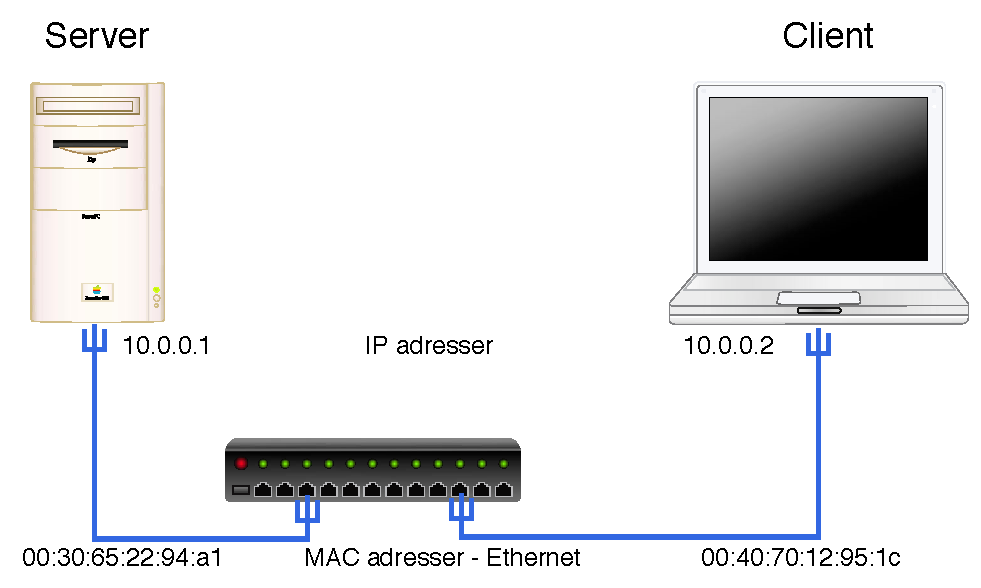
\includegraphics[width=18cm]{images/arp-basic.pdf}}  
\end{center}

%server 00:30:65:22:94:a1\\
%client 00:40:70:12:95:1c\\
%hacker 00:02:03:04:05:06\\

\slide{Hvordan virker ARP? - 2}
\begin{list1}
\item {\bfseries ping 10.0.0.2} udf�rt p� server medf�rer
\item ARP Address Resolution Protocol request/reply:
  \begin{list2}
  \item ARP request i broadcast - Who has 10.0.0.2 Tell 10.0.0.1
  \item ARP reply (fra 10.0.0.2) 10.0.0.2 is at 00:40:70:12:95:1c
  \end{list2}
\item IP ICMP request/reply:
  \begin{list2}
    \item Echo (ping) request fra 10.0.0.1 til 10.0.0.2
\item Echo (ping) reply fra 10.0.0.2 til 10.0.0.1
\item ...
  \end{list2}
\item ARP udf�res altid p� Ethernet f�r der kan sendes IP trafik
\item (kan v�re RARP til udstyr der henter en adresse ved boot)
\end{list1}


\slide{ARP cache}

\begin{alltt}
\small
hlk@bigfoot:hlk$ arp -an        
? (10.0.42.1) at 0:0:24:c8:b2:4c on en1 [ethernet]
? (10.0.42.2) at 0:c0:b7:6c:19:b on en1 [ethernet]
\end{alltt}

\begin{list1}
\item ARP cache kan vises med kommandoen \verb+arp -an+
\item -a viser alle
\item -n viser kun adresserne, pr�ver ikke at sl� navne op - typisk hurtigere
\item ARP cache er dynamisk og adresser fjernes automatisk efter 5-20 minutter hvis de ikke bruges mere
\item L�s mere med \verb+man 4 arp+
\end{list1}


\slide{Manualsystemet}

\begin{quote}
 It is a book about a Spanish guy called Manual. You should read it.
       -- Dilbert
\end{quote}

\begin{list1}
\item Manualsystemet i UNIX er utroligt st�rkt!
\item Det SKAL altid installeres sammen med v�rkt�jerne!
\item Det er n�sten identisk p� diverse UNIX varianter!  
\item \verb+man -k+ s�ger efter keyword, se ogs� \verb+apropos+
\end{list1}

Pr�v \verb+man crontab+ og \verb+man 5 crontab+

\hlkimage{10cm}{images/unix-command-1.pdf}

\slide{En manualside}

\begin{alltt}
\small
CAL(1)                BSD General Commands Manual                CAL(1)
NAME
     cal - displays a calendar
SYNOPSIS
     cal [-jy] [[month]  year]
DESCRIPTION
   cal displays a simple calendar.  If arguments are not specified, the cur-
   rent month is displayed.  The options are as follows:
   -j      Display julian dates (days one-based, numbered from January 1).
   -y      Display a calendar for the current year.

The Gregorian Reformation is assumed to have occurred in 1752 on the 3rd
of September.  By this time, most countries had recognized the reforma-
tion (although a few did not recognize it until the early 1900's.)  Ten
days following that date were eliminated by the reformation, so the cal-
endar for that month is a bit unusual.

HISTORY
     A cal command appeared in Version 6 AT&T UNIX.  
\end{alltt}

\slide{Kommandolinien p� UNIX}

\begin{list1}
\item Shells kommandofortolkere:
  \begin{list2}
    \item sh - Bourne Shell
\item bash - Bourne Again Shell
\item ksh - Korn shell, lavet af David Korn
\item csh - C shell, syntaks der minder om C sproget
\item flere andre, zsh, tcsh 
  \end{list2}
\item Svarer til command.com og cmd.exe p� Windows
\item Kan bruges som komplette programmeringssprog
\end{list1}

\slide{Kommandoprompten}


\begin{alltt}    
\small
[hlk@fischer hlk]$ id
uid=6000(hlk) gid=20(staff) groups=20(staff), 
0(wheel), 80(admin), 160(cvs) 
[hlk@fischer hlk]$ 

[root@fischer hlk]# id
uid=0(root) gid=0(wheel) groups=0(wheel), 1(daemon),
2(kmem), 3(sys), 4(tty), 5(operator), 20(staff), 
31(guest), 80(admin) 
[root@fischer hlk]#
\end{alltt}

\begin{list1}  
\item typisk viser et dollartegn at man er logget ind som almindelig bruge
\item mens en havel�ge at man er root - superbruger
\end{list1}

\slide{Kommandoliniens opbygning}


\begin{alltt}
echo [-n] [string ...]  
\end{alltt}

\begin{list1}
\item Kommandoerne der skrives p� kommandolinien skrives s�dan:
\begin{list2}
\item Starter altid med kommandoen, man kan ikke skrive \verb+henrik echo+
\item Options skrives typisk med bindestreg foran, eksempelvis \verb+-n+
\item Flere options kan s�ttes sammen, \verb+tar -cvf+ eller \verb+tar cvf+
\item I manualsystemet kan man se valgfrie options i firkantede
  klammer \verb+[]+
\item Argumenterne til kommandoen skrives typisk til sidst (eller der
  bruges redirection)
\end{list2}
\end{list1}


\slide{Adgang til UNIX}

\begin{center}

\includegraphics[width=4cm]{images/kde.png}

\includegraphics[width=4cm]{images/gnome-logo-large.png}
\end{center}

\begin{list1}
%\item Systemer der minder om UNIX kan idag nemt skaffes
\item Adgang til UNIX kan ske via grafiske brugergr�nseflader
  \begin{list2}
%  \item X11 \link{http://www.x.org}
  \item KDE \link{http://www.kde.org}
  \item GNOME \link{http://www.gnome.org}
  \end{list2}
\item eller kommandolinien
\end{list1}
\centerline{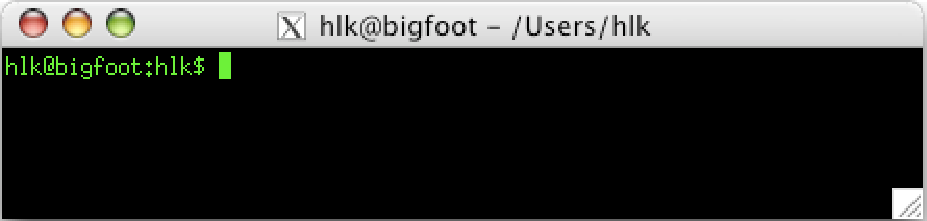
\includegraphics[width=17cm]{images/unix-cmdline.pdf}}


\exercise{ex:putty-install}


\exercise{ex:winscp-install}

\exercise{ex:unix-login}

\exercise{ex:unix-cal}

\exercise{ex:sudo}



\exercise{ex:unix-boot-cd}




\exercise{ex:unix-basic-commands}



\slide{TCP/IP basiskonfiguration}

\begin{alltt}
ifconfig en0 10.0.42.1 netmask 255.255.255.0
route add default gw 10.0.42.1 
\end{alltt}

\begin{list1}
\item konfiguration af interfaces og netv�rk p� UNIX foreg�r med:
\item \verb+ifconfig+, \verb+route+ og \verb+netstat+  
\item - ofte pakket ind i konfigurationsmenuer m.v.
\item fejls�gning foreg�r typisk med \verb+ping+ og \verb+traceroute+
\item P� Microsoft Windows benyttes ikke \verb+ifconfig+\\
men kommandoerne \verb+ipconfig+ og \verb+ipv6+
\end{list1}


\slide{Sm� forskelle}

\begin{alltt}
$ route add default 10.0.42.1
\emph{uden gw keyword!}

$ route add default gw 10.0.42.1 
\emph{Linux kr�ver gw med}
\end{alltt}

\vskip 1cm

\centerline{\bf NB: UNIX varianter kan indbyrdes v�re forskellige!}



\slide{Flere sm� forskelle}

\vskip 1cm 
\centerline{ping eller ping6}

\begin{list1}
\item Nogle systemer v�lger at ping kommandoen kan ping'e b�de IPv4 og Ipv6
\item Andre v�lger at \verb+ping+ kun benyttes til IPv4, mens IPv6 ping kaldes for \verb+ping6+
\item L�g ogs� m�rke til jargonen \emph{at pinge}
\end{list1}


\slide{OpenBSD}

Netv�rkskonfiguration p� OpenBSD:
\begin{alltt}
# cat /etc/hostname.sk0
inet 10.0.0.23 0xffffff00 NONE
# cat /etc/mygate
10.0.0.1
# cat /etc/resolv.conf    
domain security6.net
lookup file bind
nameserver 212.242.40.3
nameserver 212.242.40.51
\end{alltt}

\slide{FreeBSD}

Netv�rkskonfiguration p� FreeBSD \verb+/etc/rc.conf+:
\begin{alltt}
\small
# This file now contains just the overrides from /etc/defaults/rc.conf.
hostname="freebsd.security6.net
#ifconfig_vr0="DHCP"
ifconfig_vr0="inet 10.20.30.75 netmask 255.255.255.0"
router_enable="NO"
defaultrouter="10.20.30.65"
keyrate="fast"
moused_enable="YES"
ntpdate_enable="NO"
ntpdate_flags="none"
saver="blank"
sshd_enable="YES"
usbd_enable="YES"
...
\end{alltt}


\slide{GUI v�rkt�jer - autoconfiguration}

\hlkimage{20cm}{osx-network-automatic.png}

\slide{GUI v�rkt�jer - manuel konfiguration}

\hlkimage{20cm}{osx-network-manual.png}

\slide{ifconfig output}

\begin{alltt}\small
hlk@bigfoot:hlk$ ifconfig -a
lo0: flags=8049<UP,LOOPBACK,RUNNING,MULTICAST> mtu 16384
        inet 127.0.0.1 netmask 0xff000000 
        inet6 ::1 prefixlen 128 
        inet6 fe80::1%lo0 prefixlen 64 scopeid 0x1 
gif0: flags=8010<POINTOPOINT,MULTICAST> mtu 1280
stf0: flags=0<> mtu 1280
en0: flags=8863<UP,BROADCAST,SMART,RUNNING,SIMPLEX,MULTICAST> mtu 1500
        ether 00:0a:95:db:c8:b0 
        media: autoselect (none) status: inactive
        supported media: none autoselect 10baseT/UTP <half-duplex> 10baseT/UTP <full-duplex> 10baseT/UTP <full-duplex,hw-loopback> 100baseTX <half-duplex> 100baseTX <full-duplex> 100baseTX <full-duplex,hw-loopback> 1000baseT <full-duplex> 1000baseT <full-duplex,hw-loopback> 1000baseT <full-duplex,flow-control> 1000baseT <full-duplex,flow-control,hw-loopback>
en1: flags=8863<UP,BROADCAST,SMART,RUNNING,SIMPLEX,MULTICAST> mtu 1500
        ether 00:0d:93:86:7c:3f 
        media: autoselect (<unknown type>) status: inactive
        supported media: autoselect
\end{alltt}
%$
\vskip 1 cm
\centerline{ifconfig output er n�sten ens p� tv�rs af UNIX}




\slide{Vigtigste protokoller}


\begin{list1}
\item ARP Address Resolution Protocol
\item IP og ICMP Internet Control Message Protocol
\item UDP User Datagram Protocol
\item TCP Transmission Control Protocol
\item DHCP Dynamic Host Configuration Protocol 
\item DNS Domain Name System
\end{list1}
\vskip 1cm
\centerline{Ovenst�ende er omtrent minimumskrav for at komme p� internet}

% allerede gennemg�et ovenfor
%\slide{ICMP}

%\begin{list1}
%\item 	Internet Control Message Protocol 
%	Defineret i RFC-792

%\end{list1}


\slide{UDP User Datagram Protocol}
\hlkimage{20cm}{udp-1.pdf}
\begin{list1}
\item Forbindelsesl�s RFC-768, \emph{connection-less} - der kan tabes pakker
\item Kan benyttes til multicast/broadcast - flere modtagere
\end{list1}



\slide{TCP Transmission Control Protocol}
\hlkimage{20cm}{tcp-1.pdf}

\begin{list1}
\item Forbindelsesorienteret RFC-791 September 1981, \emph{connection-oriented}
\item Enten overf�res data eller man f�r fejlmeddelelse
\end{list1}




\slide{TCP three way handshake}

\hlkimage{7cm}{images/tcp-three-way.pdf}

\begin{list2}
\item {\bfseries TCP SYN half-open} scans
\item Tidligere loggede systemer kun n�r der var etableret en fuld TCP
  forbindelse - dette kan/kunne udnyttes til \emph{stealth}-scans
\item Hvis en maskine modtager mange SYN pakker kan dette fylde
  tabellen over connections op - og derved afholde nye forbindelser
  fra at blive oprette - {\bfseries SYN-flooding}
\end{list2}

\slide{Well-known port numbers}

\hlkimage{10cm}{iana1.jpg}

\begin{list1}
\item IANA vedligeholder en liste over magiske konstanter i IP
\item De har lister med hvilke protokoller har hvilke protokol ID m.v.
\item En liste af interesse er port numre, hvor et par eksempler er:
\begin{list2}
\item Port 25 SMTP Simple Mail Transfer Protocol
\item Port 53 DNS Domain Name System
\item Port 80 HTTP Hyper Text Transfer Protocol over TLS/SSL
\item Port 443 HTTP over TLS/SSL
\end{list2}
\item Se flere p� \link{http://www.iana.org}
\end{list1}

\slide{Hierarkisk routing}

\hlkimage{18cm}{routing-1.pdf}
Hvordan kommer pakkerne frem til modtageren

\slide{IP default gateway}

\hlkimage{13cm}{routing-2.pdf}

\begin{list1}
\item IP routing er nemt
\item En host kender en default gateway i n�rheden
\item En router har en eller flere upstream routere, f� adresser den sender videre til
\item Core internet har default free zone, kender \emph{alle netv�rk} 
\end{list1}



\slide{DHCP Dynamic Host Configuration Protocol}

\hlkimage{13cm}{dhcp-1.pdf}

\begin{list1}
\item Hvordan f�r man information om default gateway
\item Man sender et DHCP request og modtager et svar fra en DHCP server
\item Dynamisk konfiguration af klienter fra en centralt konfigureret server
\item Bruges til IP adresser og meget mere
\end{list1}


\slide{Routing}


\begin{list1}
  \item routing table - tabel over netv�rkskort og tilh�rende adresser
\item default gateway - den adresse hvortil man sender
  \emph{non-local} pakker\\kaldes ogs� default route, gateway of last
  resort
\item routing styres enten manuelt - opdatering af route tabellen,
  eller konfiguration af adresser og subnet maske p� netkort
\item eller automatisk ved brug af routing protocols - interne og
  eksterne route protokoller
\item de lidt �ldre routing protokoller har ingen sikkerhedsmekanismer
\item {\bf IP benytter longest match i routing tabeller!}
\item Den mest specifikke route g�lder for forward af en pakke!
\end{list1}


\slide{Routing forst�else}

\begin{alltt}
\small
$ netstat -rn
Routing tables

Internet:
Destination    Gateway         Flags  Refs      Use  Netif 
default        10.0.0.1        UGSc    23        7    en0
10/24          link#4          UCS      1        0    en0
10.0.0.1       0:0:24:c1:58:ac UHLW    24       18    en0  
10.0.0.33      127.0.0.1       UHS      0        1    lo0
10.0.0.63      127.0.0.1       UHS      0        0    lo0
127            127.0.0.1       UCS      0        0    lo0
127.0.0.1      127.0.0.1       UH       4     7581    lo0
169.254        link#4          UCS      0        0    en0  
\end{alltt}

\vskip 1 cm
\centerline{Start med kun at se p� Destination, Gateway og Netinterface}


\exercise{ex:network-ifconfig}
\exercise{ex:network-netstat}
\exercise{ex:network-lsof}


\slide{whois systemet}

\begin{list1}
\item IP adresserne administreres i dagligdagen af et antal Internet
  registries, hvor de st�rste er:
\begin{list2}
\item RIPE (R�seaux IP Europ�ens)  \link{http://ripe.net}
\item ARIN American Registry for Internet Numbers \link{http://www.arin.net}
\item Asia Pacific Network Information Center \link{http://www.apnic.net}
\item LACNIC (Regional Latin-American and Caribbean IP Address Registry) - Latin America and some Caribbean Islands
\end{list2}
\item disse fire kaldes for Regional Internet Registries (RIRs) i
  mods�tning til Local Internet Registries (LIRs) og National Internet
  Registry (NIR) 
\end{list1}

\slide{whois systemet-2}

\begin{list1}
\item ansvaret for Internet IP adresser ligger hos ICANN The Internet
  Corporation for Assigned Names and Numbers\\
\link{http://www.icann.org}
\item NB: ICANN m� ikke forveksles med IANA Internet Assigned Numbers
  Authority \link{http://www.iana.org/} som bestyrer portnumre m.v.
\end{list1}

\exercise{ex:whois}


% basic ping og traceroute

\slide{Ping}

\begin{list1}
\item ICMP - Internet Control Message Protocol
\item Benyttes til fejlbeskeder og til diagnosticering af forbindelser
\item ping programmet virker ved hj�lp af ICMP ECHO request og
  forventer ICMP ECHO reply
\item 
\begin{alltt}
\small {\bfseries 
$ ping 192.168.1.1}
PING 192.168.1.1 (192.168.1.1): 56 data bytes
64 bytes from 192.168.1.1: icmp_seq=0 ttl=150 time=8.849 ms
64 bytes from 192.168.1.1: icmp_seq=1 ttl=150 time=0.588 ms
64 bytes from 192.168.1.1: icmp_seq=2 ttl=150 time=0.553 ms
\end{alltt}
\end{list1}

\slide{traceroute}

\begin{list1}
  \item traceroute programmet virker ved hj�lp af TTL
\item levetiden for en pakke t�lles ned i hver router p� vejen og ved at s�tte denne lavt
  opn�r man at pakken \emph{timer ud} - besked fra hver router p� vejen
\item default er UDP pakker, men p� UNIX systemer er der ofte mulighed
  for at bruge ICMP
\item 
\begin{alltt}
\small{\bfseries 
$ traceroute 217.157.20.129}
traceroute to 217.157.20.129 (217.157.20.129),
30 hops max, 40 byte packets
 1  safri (10.0.0.11)  3.577 ms  0.565 ms  0.323 ms
 2  router (217.157.20.129)  1.481 ms  1.374 ms  1.261 ms
\end{alltt}
\end{list1}

%DNS
\slide{Domain Name System}

\hlkimage{12cm}{dns-1.pdf}

\begin{list1}
\item Gennem DHCP f�r man typisk ogs� information om DNS servere
\item En DNS server kan sl� navne, dom�ner og adresser op
\item Foreg�r via query og response med datatyper kaldet resource records
\item DNS er en distribueret database, s� opslag kan resultere i flere opslag
\end{list1}


\slide{DNS systemet}

\begin{list1}
\item navneopslag p� Internet  
\item tidligere brugte man en {\bfseries hosts} fil\\
hosts filer bruges stadig lokalt til serveren - IP-adresser
\item UNIX: /etc/hosts
\item Windows \verb+c:\windows\system32\drivers\etc\hosts+
\item Eksempel: www.security6.net har adressen 217.157.20.131
\item skrives i database filer, zone filer
\end{list1}

\begin{alltt}
ns1     IN      A       217.157.20.130
        IN      AAAA    2001:618:433::1
www     IN      A       217.157.20.131
        IN      AAAA    2001:618:433::14
\end{alltt}

\slide{Mere end navneopslag}

\begin{list1}
  \item best�r af resource records med en type:
    \begin{list2}
\item adresser A-records
\item IPv6 adresser AAAA-records
\item autoritative navneservere NS-records
\item post, mail-exchanger MX-records
\item flere andre: md ,  mf ,  cname ,  soa ,
                  mb , mg ,  mr ,  null ,  wks ,  ptr ,
                  hinfo ,  minfo ,  mx ....
\end{list2}
\end{list1}
\begin{alltt}
        IN      MX      10      mail.security6.net.
        IN      MX      20      mail2.security6.net.
\end{alltt}

\slide{Basal DNS ops�tning p� klienter}

\begin{list1}    
\item \verb+/etc/resolv.conf+
\item NB: denne fil kan hedde noget andet p� UNIX varianter!
\item eksempelvis \verb+/etc/netsvc.conf+
\item typisk indhold er dom�nenavn og IP-adresser for navneservere
\end{list1}

\begin{alltt}
domain security6.net
nameserver 212.242.40.3
nameserver 212.242.40.51
\end{alltt}

\slide{DNS root servere}
\begin{list1}
  \item Root-servere - 13 stk geografisk distribueret fordelt p� Internet
\end{list1}

\begin{alltt}
I.ROOT-SERVERS.NET.     3600000 A       192.36.148.17
E.ROOT-SERVERS.NET.     3600000 A       192.203.230.10
D.ROOT-SERVERS.NET.     3600000 A       128.8.10.90
A.ROOT-SERVERS.NET.     3600000 A       198.41.0.4
H.ROOT-SERVERS.NET.     3600000 A       128.63.2.53
C.ROOT-SERVERS.NET.     3600000 A       192.33.4.12
G.ROOT-SERVERS.NET.     3600000 A       192.112.36.4
F.ROOT-SERVERS.NET.     3600000 A       192.5.5.241
B.ROOT-SERVERS.NET.     3600000 A       128.9.0.107
J.ROOT-SERVERS.NET.     3600000 A       198.41.0.10
K.ROOT-SERVERS.NET.     3600000 A       193.0.14.129
L.ROOT-SERVERS.NET.     3600000 A       198.32.64.12
M.ROOT-SERVERS.NET.     3600000 A       202.12.27.33  
\end{alltt}

\slide{DK-hostmaster}

\begin{list1}
\item bestyrer .dk TLD - top level domain
  
\item man registrerer ikke .dk-dom�ner hos DK-hostmaster, men hos en
  registrator 
\item Et dom�ne b�r have flere navneservere og flere postservere
\item autoritativ navneserver - ved autoritativt om IP-adresse for
  maskine.dom�ne.dk findes 
\item ikke-autoritativ - har p� vegne af en klient sl�et en adresse op
\item Det anbefales at overveje en service som
  \link{http://www.gratisdns.dk} der har 5 navneservere distribueret
  over stor geografisk afstand - en udenfor Danmark
\end{list1}

\slide{Navngivning af servere}

\begin{list1}
  \item Hvordan skal vi kunne huske og administrere servere?
\item Det er ikke nemt at navngive hverken brugere eller servere!
\item Selvom det lyder smart med A01S13, som forkortelse af Afdeling
  01's Server nr 13, er det umuligt at huske
\item ... men m�ske n�dvendigt i de st�rste netv�rk
  \begin{list2}
  
\item Windows serveren er dom�necontroller - skal hedde:
\item Linux server som er terminalserver - skal hedde:
\item PC-system med NetBSD skal m�ske v�re vores ene server - skal hedde: ?
\item PC-system 1 med en Linux server - skal hedde: 
\item PC-system 2 med en Linux server - skal hedde:
  \end{list2}
\end{list1}



% NAT
\slide{NAT Network Address Translation}
\hlkimage{20cm}{nat-1.pdf}


\vskip 2 cm
\begin{list2}
\item NAT bruges til at forbinde et privat net (RFC-1918 adresser) med internet
\item NAT gateway udskifter afsender adressen med sin egen
\item En quick and dirty fix der vil forf�lge os for resten af vores
  liv 
\item �del�gger en del protokoller :-(
\item L�gger state i netv�rket - �del�gger fate sharing  
\end{list2}




\slide{NAT is BAD}


\hlkimage{20cm}{nat-is-bad.pdf}


\begin{list2}
\item NAT �del�gger end-to-end transparency!
\item Problemer med servere bagved NAT
\item "l�ser" problemet "godt nok" (tm) for mange
\item Men idag ser vi multilevel NAT! - eeeeeeewwwwww!
\item Se RFC-2775 Internet Transparency for mere om dette emne
\end{list2}


\exercise{ex:ping}
\exercise{ex:icmpush}
\exercise{ex:basic-dns-lookup}



\slide{Agenda - dag 2 Avancerede netv�rksteknologier og 802.11}
%\hlkimage{18cm}{nagios-status-overview.jpg}
\hlkimage{21cm}{cricket-mini-graph.png}


\slide{Nu skal vi til management og diagnosticering}

\begin{list1}
\item Always check the spark plugs!
\item N�r man skal spore fejl i netv�rk er det essentielt at starte fra bunden:
\begin{list2}
\item Er der link?
\item Er der IP-adresse?
\item Er der route?
\item Modtager systemet pakker
\item Er der en returvej fra systemet! Den her kan snyde mange!
\item Lytter serveren p� den port man vil forbinde til, UDP/TCP
\end{list2} 
\item Hvis der ikke er link vil man aldrig f� svar fra databasen/webserveren/postserveren
\end{list1}

\slide{Udtr�k af netv�rkskonfigurationen}

\begin{list1}
\item De vigtigste kommandoer til udtr�k af netv�rkskonfigurationen
\item P� Unix:
\begin{list2}
\item cat - til at vise tekstfiler
\item ifconfig - interface configuration
\item netstat - network statistics
\item lsof - list open files
\end{list2}
\item Windows:
\begin{list2}
\item kontrolpanelet
\item ipconfig/ipv6
\end{list2}
\end{list1}

\slide{Basale testv�rkt�jer TCP - Telnet og OpenSSL}

\begin{list1}
\item Telnet blev tidligere brugt til login og er en klartekst forbindelse
over TCP
\item Telnet kan bruges til at teste forbindelsen til mange �ldre serverprotokoller som benytter ASCII kommandoer
\begin{list2}
\item \verb+telnet mail.kramse.dk 25+ laver en forbindelse til port 25/tcp
\item \verb+telnet www.kramse.dk 80+ laver en forbindelse til port 80/tcp
\end{list2}
\item Til krypterede forbindelser anbefales det at teste med openssl
\begin{list2}
\item \verb+openssl s_client -host www.kramse.dk -port 443+\\
laver en forbindelse til port 443/tcp med SSL
\item \verb+openssl s_client -host mail.kramse.dk -port 993+\\
 laver en forbindelse til port 993/tcp med SSL
\end{list2}
\item Med OpenSSL i client-mode kan services tilg�s med samme tekstkommandoer som med telnet
\end{list1}


\slide{Basale testv�rkt�jer UDP}

\begin{list1}
\item UDP er lidt drilsk, for de fleste services er ikke \emph{ASCII protokoller}
\item Der findes dog en r�kke testprogrammer, a la ping
\begin{list2}
\item nsping - name server ping
\item dhcping - dhcp server ping
\item ...
\end{list2}
\item Derudover kan man bruge de s�dvanlige programmer som \verb+host+ til navneopslag osv.
\end{list1}


\slide{Logfiler}
\begin{list1}
\item Logfiler er en n�dvendighed for at have et transaktionsspor
\item Logfiler giver mulighed for statistik
\item Logfiler er desuden n�dvendige for at fejlfinde
\item Det kan v�re relevant at sammenholde logfiler fra:  
\begin{list2}
\item routere
\item firewalls
\item webservere
\item intrusion detection systemer
\item adgangskontrolsystemer
\item ...
\end{list2}
\item Husk - tiden er vigtig! Network Time Protocol (NTP) anbefales 
\item Husk at logfilerne typisk kan slettes af en angriber -
  hvis denne f�r kontrol med systemet
\end{list1}


\slide{syslog}

\begin{list1}
\item syslog er system loggen p� Unix og den er effektiv
  \begin{list2}
\item man kan definere hvad man vil se og hvor man vil have det
  dirigeret hen
\item man kan samle det i en fil eller opdele alt efter programmer og
  andre kriterier
\item man kan ligeledes bruge named pipes - dvs filer i filsystemet
  som tunneller fra chroot'ed services til syslog i det centrale system! 
\item man kan nemt sende data til andre systemer
  \end{list2}
\item Hvis man vil lave en centraliseret l�sning er f�lgende link
  vigtigt: \\
\link{http://loganalysis.org}
\end{list1}

\slide{syslogd.conf eksempel}
\begin{alltt}
\small
*.err;kern.debug;auth.notice;authpriv.none;mail.crit    /dev/console
*.notice;auth,authpriv,cron,ftp,kern,lpr,mail,user.none /var/log/messages
kern.debug;user.info;syslog.info                        /var/log/messages
auth.info                                               /var/log/authlog
authpriv.debug                                          /var/log/secure
...
# Uncomment to log to a central host named "loghost".
#*.notice;auth,authpriv,cron,ftp,kern,lpr,mail,user.none        @loghost
#kern.debug,user.info,syslog.info                               @loghost
#auth.info,authpriv.debug,daemon.info                           @loghost
\end{alltt}

\slide{Andre syslogs syslog-ng}

\begin{list1}
\item der findes andre syslog systemer eksempelvis syslog-ng
\item konfigureres gennem \verb+/etc/syslog-ng/syslog-ng.conf+   
\item Eksempel p� indholdet af filen kunne v�re:
\end{list1}

\begin{alltt}
\small 
options \{ 
        long_hostnames(off); 
        sync(0); 
        stats(43200); 
\};

source src { unix-stream("/dev/log"); internal(); pipe("/proc/kmsg"); };
destination messages { file("/var/log/messages"); };
destination console_all { file("/dev/console"); };
log { source(src); destination(messages); };
log { source(src); destination(console_all); };
\end{alltt}

\exercise{ex:syslogd-basic}

\slide{Logfiler og computer forensics}
\begin{list1}
\item Logfiler er en n�dvendighed for at have et transaktionsspor
\item Logfiler er desuden n�dvendige for at fejlfinde
\item Det kan v�re relevant at sammenholde logfiler fra:  
\begin{list2}
\item routere
\item firewalls
\item intrusion detection systemer
\item adgangskontrolsystemer
\item ...
\end{list2}
\item Husk - tiden er vigtig! Network Time Protocol (NTP) anbefales 
\item Husk at logfilerne typisk kan slettes af en angriber -
  hvis denne f�r kontrol med systemet
\end{list1}


\slide{Simple Network Management Protocol}

\begin{list1}
\item SNMP er en protokol der supporteres af de fleste professionelle
  netv�rksenheder, s�som switche, routere
\item hosts - skal sl�s til men f�lger som regel med
\item SNMP bruges til: 
  \begin{list2}
    \item \emph{network management}
    \item statistik
    \item rapportering af fejl - SNMP traps
  \end{list2}
\item {\bfseries sikkerheden baseres p� community strings der sendes
    som klartekst ...}
\item det er nemmere at brute-force en community string end en
  brugerid/kodeord kombination
\end{list1}

\slide{SNMP - \emph{hacking}}

\vskip 2 cm

\begin{list1}
\item Simple Network Management Protocol
\item sikkerheden afh�nger alene af en Community string SNMPv2
\item typisk er den nem at g�tte:
  \begin{list2}
    \item public - default til at afl�se statistik
\item private - default n�r man skal �ndre p� enheden, skrive 
\item cisco
\item ...
  \end{list2}
\item Der findes lister og ordb�ger p� nettet over kendte default communities
\end{list1}

\slide{Systemer med SNMP}

\begin{list1}
  \item kan v�re sv�rt at finde ... det er UDP 161
\item Hvis man finder en s� pr�v at bruge {\bfseries snmpwalk}
  programmet - det kan vise alle tilg�ngelige SNMP oplysninger fra den
  p�g�ldende host 
\item det kan v�re en af m�derne at identificere uautoriserede WLAN
  Access Points p� - sweep efter port 161/UDP 
\item snmpwalk er et af de mest brugte programmer til at hente snmp
  oplysninger - i forbindelse med hackning og penetrationstest
\end{list1}

\slide{snmpwalk}

\begin{list1}
\item Typisk brug er:
\item \verb+snmpwalk -v 1 -c secret switch1+
\item \verb+snmpwalk -v 2c -c secret switch1+
\item Eventuelt bruges \verb+snmpget+ og \verb+snmpset+
\item Ovenst�ende er en del af Net-SNMP pakken\\
 \link{http://net-snmp.sourceforge.net/}
\end{list1}

\exercise{ex:snmpwalk}


\slide{Eksempler p� SNMP og management}

\begin{list1}
\item Ofte foreg�r administration af netv�rksenheder via HTTP, Telnet eller SSH
\begin{list2}	
\item sm� dumme enheder er idag ofte web-enablet
\item bedre enheder giver b�de HTTP og kommandolinieadgang
\item de bedste giver mulighed for SSH, fremfor Telnet
\end{list2}
\end{list1}


\slide{Tobi Oetiker's MRTG The Multi Router Traffic Grapher}

\hlkimage{15cm}{rrdtool-demo.png}

\begin{list1}
\item Monitorering af SNMP enheder og grafer
\item Inkluderer en nem configmaker og benytter idag RRDTool til data
\item Hjemmesiden: \link{http://oss.oetiker.ch/mrtg/}
\end{list1}

\slide{RRDTool Round Robin Database Tool}

\hlkimage{12cm}{rrdtool-demo.png}

\begin{list1}
\item Round Robin Database Tool er en m�de at gemme data p�
\item Med RRDTool kan man derefter f� lavet grafer
\item Typisk bruger man et andet v�rkt�j som benytter RRDTool til data
\item \link{http://oss.oetiker.ch/rrdtool/doc/index.en.html}
\end{list1}

Kan bruges til temperaturm�linger og alt muligt andet

\slide{Smokeping}

\hlkimage{15cm}{smokeping-demo.jpg}

\begin{list1}
\item M�ling af latency for netv�rksservice
\item Underst�tter et stort antal prober: ICMP, DNS, HTTP, LDAP, SMTP, ...
\item Min SmokePing server \link{http://pumba.kramse.dk/smokeping/}
\item Hjemmesiden for SmokePing \link{http://oss.oetiker.ch/smokeping/}
\item Lavet af Tobias Oetiker og Niko Tyni
\end{list1}


\slide{Nagios}

\begin{list1}
\item Overv�gningsv�rkt�j der giver godt overblik
\begin{list2}	
\item Monitoring af diverse services (SMTP, POP3, HTTP, NNTP, PING, etc.)
\item Monitoring af host resources (processor load, disk and memory usage, running processes, log files, etc.)
\item Monitoring af andre ressourcer som temperatur
\item Simpel plugin design som g�r det nemt at udvide
\item Kan sende e-mail, SMS m.v.
\end{list2}
\item Benyttes mange steder
\item Hjemmesiden for Nagios \link{http://www.nagios.org/}
\end{list1}

\slide{Stop - overv�gningsv�rkt�jer}

\begin{list1}
\item Brug lidt tid p� at se p� vores netv�rk
\item Valgfrit om I vil se p� Administrationsinterface p� switche
\item eller SNMP indstillinger eksempelvis
\item eller Nagios og SmokePing p� mine servere
\end{list1}


\slide{Sm� DNS tools bind-version - Shell script}

\begin{alltt}\small
#! /bin/sh
# Try to get version info from BIND server
PROGRAM=`basename $0`
. `dirname $0`/functions.sh
if [ $# -ne 1 ]; then
   echo "get name server version, need a target! "
   echo "Usage: $0 target"
   echo "example $0 10.1.2.3"
   exit 0
fi
TARGET=$1
# using dig 
start_time
dig @$1 version.bind chaos txt
echo Authors BIND er i versionerne 9.1 og 9.2 - m�ske ...
dig @$1 authors.bind chaos txt
stop_time
\end{alltt}
\centerline{\link{http://www.kramse.dk/files/tools/dns/bind-version}}

\slide{Sm� DNS tools dns-timecheck - Perl script}

\begin{alltt}\small
#!/usr/bin/perl
# modified from original by Henrik Kramsh�j, hlk@kramse.dk
# 2004-08-19
#
# Original from: http://www.rfc.se/fpdns/timecheck.html
use Net::DNS;

my $resolver = Net::DNS::Resolver->new;
$resolver->nameservers($ARGV[0]);

my $query = Net::DNS::Packet->new;
$query->sign_tsig("n","test");

my $response = $resolver->send($query);
foreach my $rr ($response->additional) {
  print "localtime vs nameserver $ARGV[0] time difference: ";
  print$rr->time_signed - time() if $rr->type eq "TSIG";
}  
\end{alltt}
% inserting stupid $ to stop EMACS from
\centerline{\link{http://www.kramse.dk/files/tools/dns/dns-timecheck}}



\exercise{ex:bind-version}


% 802.11 her
\slide{Tr�dl�se teknologier 802.11}

\begin{list1}
\item 802.11 er arbejdsgruppen under IEEE 
\item De mest kendte standarder idag indenfor tr�dl�se teknologier:
\begin{list2}
\item 802.11b 11Mbps versionen
\item 802.11g 54Mbps versionen
\item 802.11n endnu hurtigere, og draft
\item 802.11i Security enhancements
\end{list2}
\item Der er propriet�re versioner 22Mbps og den slags\\
- det anbefales IKKE at benytte disse da det giver vendor lock-in -
man bliver l�st fast
\end{list1}

Kilde: \link{http://grouper.ieee.org/groups/802/11/index.html}

\slide{802.11 modes og frekvenser}

\begin{list1}
\item Access point k�rer typisk i \emph{access point mode} ogs� kaldet
  infrastructure mode - al trafik g�r via AP
\item Alternativt kan wireless kort oprette ad-hoc netv�rk - hvor
  trafikken g�r direkte mellem netkort
\item Frekvenser op til kanal 11 og 12+13 i DK/EU
\item Helst 2 kanaler spring for 802.11b AP der placeres indenfor r�kkevidde
\item Helst 4 kanaler spring for 802.11g AP der placeres indenfor r�kkevidde
\end{list1}

\slide{Eksempel p� netv�rk med flere AP'er}

\hlkimage{20cm}{images/wireless-multi-ap.pdf}

\slide{Eksempel p� netv�rk med flere AP'er}

\hlkimage{20cm}{images/wireless-multi-ap-2.pdf}


\slide{Wireless Distribution System WDS}

\hlkimage{18cm}{images/wireless-multi-ap-wds.pdf}

\begin{list1}
\item Se ogs�:
\link{http://en.wikipedia.org/wiki/Wireless_Distribution_System}
\end{list1}


\slide{\hskip 1 cm Er tr�dl�se netv�rk interessante?}

\begin{list1}
\item Sikkerhedsproblemer i de tr�dl�se netv�rk er mange
  \begin{list2}
  \item Fra lavt niveau - eksempelvis ARP, 802.11
  \item d�rlige sikringsmekanismer - WEP
  \item d�rligt udstyr - mange fejl
  \item usikkkerhed om implementering og overv�gning
  \end{list2}
\item Tr�dl�st udstyr er blevet meget billigt!
\item Det er et krav fra brugerne - tr�dl�st er l�kkert
\end{list1}


\slide{Konsekvenserne}

\hlkimage{10cm}{images/wireless-daekning.pdf}

\begin{list2}
\item V�rre end Internetangreb - anonymt
\item Kr�ver ikke fysisk adgang til lokationer
%\emph{spioneres imod}
\item Konsekvenserne ved sikkerhedsbrud er generelt st�rre
\item Typisk f�r man direkte LAN eller Internet adgang!
\end{list2}



\slide{Konsulentens udstyr wireless}

\begin{list1}
\item Laptop gerne med PC-CARD slot
\item Tr�dl�se kort Atheros, de indbyggede er ofte ringe ;-)
\item Access Points - jeg anbefaler Airport Express
\item Antenner hvis man har lyst
\item B�ger: \emph{Real 802.11 security}
\item Internetressourcer:
\begin{list2}
\item BackTrack - CD image med Linux+v�rkt�jer    
\item Packetstorm wireless tools
\link{http://packetstormsecurity.org/wireless/}
\item \emph{Beginner's Guide to Wireless Auditing}
David Maynor \\
\link{http://www.securityfocus.com/infocus/1877?ref=rss}
\item Aircrack-ng suiten af programmer \link{http://www.aircrack-ng.org/}
\end{list2}
\end{list1}


\slide{Typisk brug af 802.11 udstyr}

\begin{center}
\colorbox{white}{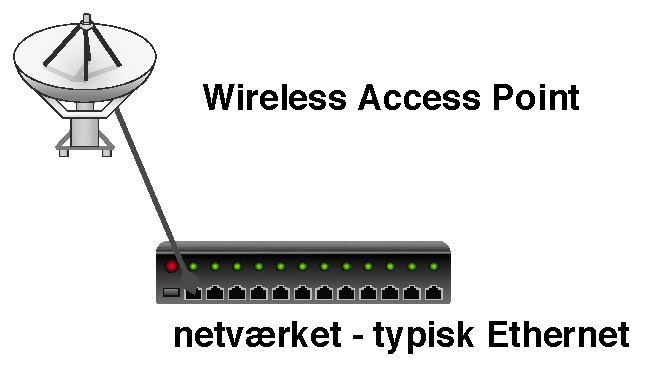
\includegraphics[width=20cm]{images/wlan-accesspoint-1.pdf}}
\end{center}

\centerline{\hlkbig et access point - forbindes til netv�rket}

\slide{Basal konfiguration}

\begin{list1}
\item N�r man tager fat p� udstyr til tr�dl�se netv�rk opdager man:
\item SSID - nettet skal have et navn
\item frekvens / kanal - man skal v�lge en kanal, eller udstyret
  v�lger en automatisk
\item der er nogle forskellige metoder til sikkerhed  
\end{list1}


\exercise{ex:AirPort-AP}

\slide{Tr�dl�s sikkerhed}

\hlkimage{14cm}{images/apple-wireless-security.png}

\begin{list2}
\item Tr�dl�s sikkerhed - WPA og WPA2
\item Nem konfiguration
\item Nem konfiguration af Access Point  
\end{list2}

\slide{Wireless networking sikkerhed i 802.11b}

\hlkimage{10cm}{images/wlan-accesspoint-1.pdf}

\begin{list1}
\item Sikkerheden er baseret p� nogle f� foruds�tninger 
  \begin{list2}
  \item SSID - netnavnet
  \item WEP \emph{kryptering} - Wired Equivalent Privacy
  \item m�ske MAC flitrering, kun bestemte kort m� tilg� accesspoint 
  \end{list2}
\item Til geng�ld er disse foruds�tninger ofte ikke tilstr�kkelige ... 
%\item Hvorfor hader du WEP?
  \begin{list2}
  \item WEP er m�ske \emph{ok} til visse sm� hjemmenetv�rk
  \item WEP er baseret p� en DELT hemmelighed som alle stationer kender
  \item n�glen �ndres sj�ldent, og det er sv�rt at distribuere en ny
  \end{list2}
  
\end{list1}


\slide{Foruds�tninger}

\begin{list1}
\item Til geng�ld er disse foruds�tninger ofte ikke tilstr�kkelige ... 
\item Hvad skal man beskytte?
\item Hvordan kan sikkerheden omg�s?
\item Mange firmaer og virksomheder stille forskellige krav til
  sikkerheden - der er ikke en sikkerhedsmekanisme der passer til alle
\end{list1}

\slide{SSID - netnavnet}

\begin{list1}
\item Service Set Identifier (SSID) - netnavnet
\item 32 ASCII tegn eller 64 hexadecimale cifre
\item Udstyr leveres typisk med et standard netnavn
\begin{list2}
\item Cisco - tsunami
\item Linksys udstyr - linksys
\item Apple Airport, 3Com m.fl. - det er nemt at genkende dem  
\end{list2}
\item SSID kaldes ogs� for NWID - network id
\item SSID broadcast - udstyr leveres oftest med broadcast af SSID
\end{list1}


%wardriving her
\slide{Demo: wardriving med stumbler programmer}

\hlkimage{17cm}{images/macstumbler.png}  

\begin{list1}
\item man tager et tr�dl�st netkort og en b�rbar computer og noget software:
\begin{list2}
\item Netstumbler - Windows \link{http://www.netstumbler.com}
\item dstumbler - UNIX \link{http://www.dachb0den.com/projects/dstumbler.html}
\item iStumbler - Mac \link{http://www.istumbler.net/}
\item Kismet ... mange andre
  \end{list2}
\end{list1}

\slide{Start p� demo - wardriving}

\hlkimage{15cm}{images/server-client-wlan.pdf}

\begin{list2}
\item Almindelige laptops bruges til demo
\item Der startes et \emph{access point}
\end{list2}

\slide{MAC filtrering}

\begin{list1}
\item De fleste netkort tillader at man udskifter sin MAC adresse
\item MAC adressen p� kortene er med i alle pakker der sendes
\item MAC adressen er aldrig krypteret, for hvordan skulle pakken s�
  n� frem?
\item MAC adressen kan derfor overtages, n�r en af de tilladte
  stationer forlader omr�det ...
\end{list1}

\slide{Resultater af wardriving}

\begin{list1}
\item Hvad opdager man ved wardriving?
\begin{list2}
\item at WEP IKKE krypterer hele pakken
\item at alle pakker indeholder MAC adressen
\item WEP n�glen skifter sj�ldent
\item ca. 2/3 af de netv�rk man finder har ikke WEP sl�et til - og der
  er fri og uhindret adgang til Internet
\end{list2}
\item {\color{red}
Man kan alts� lytte med p� et netv�rk med WEP, genbruge en anden
maskines MAC adresse - og m�ske endda bryde WEP krypteringen.}
\item 
Medmindre man kender virksomheden og WEP n�glen ikke er skiftet ...
det er besv�rligt at skifte den, idet alle stationer skal opdateres.
\end{list1}

\slide{Stork�benhavn}

\begin{center}
\colorbox{white}{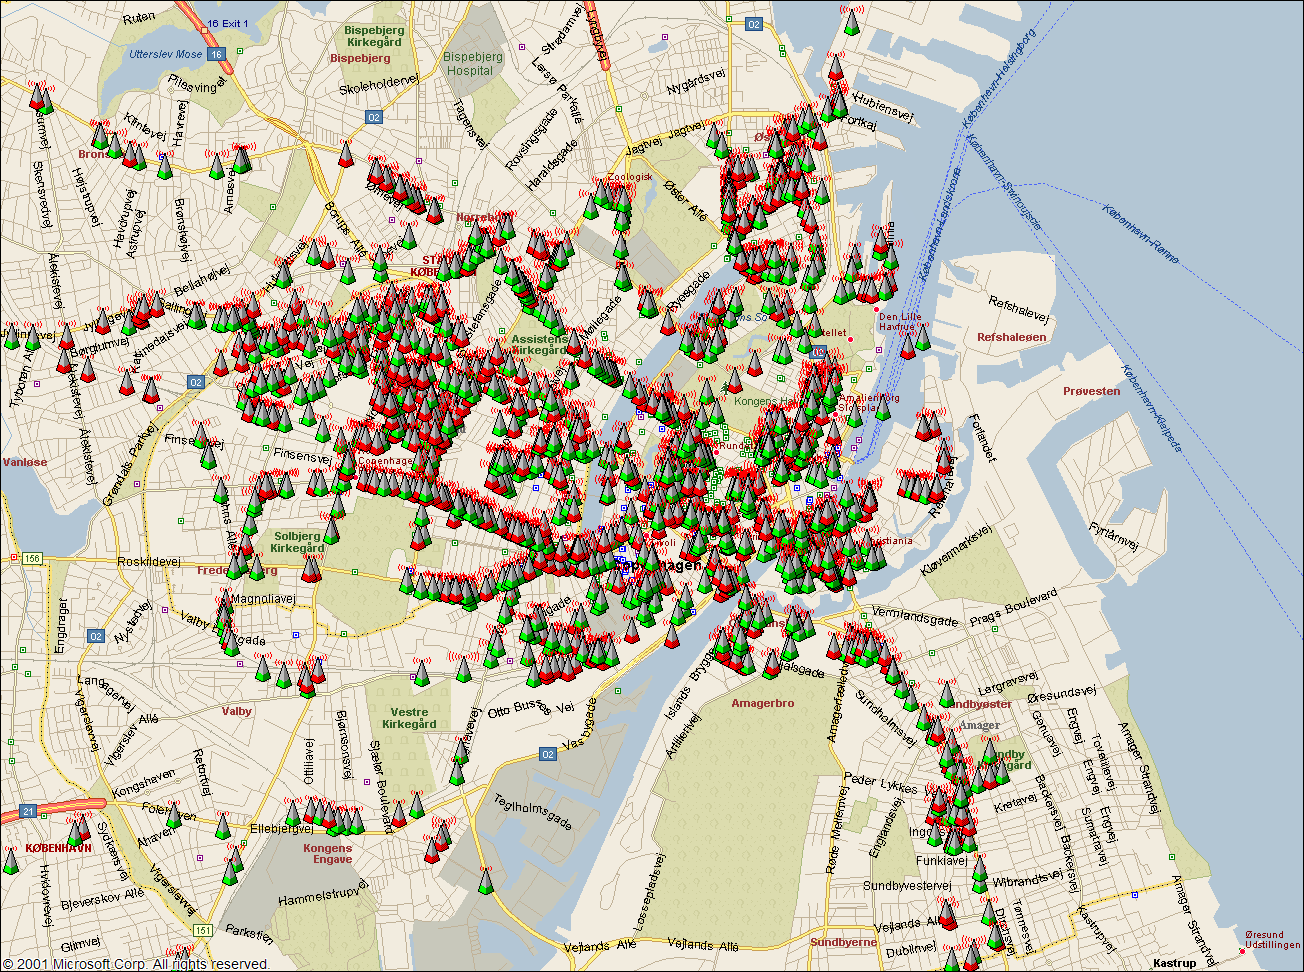
\includegraphics[width=20cm]{images/20030830-kbh.png}}  
\end{center}

\exercise{ex:wardriving-windows}
\exercise{ex:wardriving-kismet}

\slide{Informationsindsamling}

\begin{list1}
\item Det vi har udf�rt er informationsindsamling
\item Indsamlingen kan v�re aktiv eller passiv indsamling i forhold
  til m�let for angrebet
\item passiv kunne v�re at lytte med p� trafik eller s�ge i databaser
  p� Internet
\item aktiv indsamling er eksempelvis at sende ICMP pakker og
  registrere hvad man f�r af svar
\end{list1}

\slide{WEP kryptering} 

%\begin{center}
%\colorbox{white}{
\includegraphics[width=12cm]{images/airsnort.pdf}}  
%\end{center}
\begin{list1}
\item WEP \emph{kryptering} - med n�gler der specificeres som tekst
  eller hexadecimale cifre
\item typisk 40-bit, svarende til 5 ASCII tegn eller 10 hexadecimale
  cifre eller 104-bit 13 ASCII tegn eller 26 hexadecimale cifre
\item WEP er baseret p� RC4 algoritmen der er en \emph{stream cipher}
  lavet af Ron Rivest for RSA Data Security
\end{list1}


\slide{De f�rste fejl ved WEP}
\begin{list1}
\item Oprindeligt en d�rlig implementation i mange Access Points
\item Fejl i krypteringen - rettet i nyere firmware
\item WEP er baseret p� en DELT hemmelighed som alle stationer kender
\item N�glen �ndres sj�ldent, og det er sv�rt at distribuere en ny
\end{list1}


\slide{WEP sikkerhed}

\hlkimage{12cm}{images/airsnort.pdf}  

\begin{quote}
AirSnort is a wireless LAN (WLAN) tool which recovers encryption
keys. AirSnort operates by passively monitoring transmissions,
computing the encryption key when enough packets have been gathered.  

802.11b, using the Wired Equivalent Protocol (WEP), is crippled with
numerous security flaws. Most damning of these is the weakness
described in " Weaknesses in the Key Scheduling Algorithm of RC4 "
by Scott Fluhrer, Itsik Mantin and Adi Shamir. Adam Stubblefield
was the first to implement this attack, but he has not made his
software public. AirSnort, along with WEPCrack, which was released
about the same time as AirSnort, are the first publicly available
implementaions of this attack.  \link{http://airsnort.shmoo.com/}
\end{quote}

%\begin{list1}
%\item i dag er firmware opdateret hos de fleste producenter
%\item men sikkerheden baseres stadig p� een delt hemmelighed
%\end{list1}

\slide{major cryptographic errors}

\begin{list1}
\item weak keying - 24 bit er allerede kendt - 128-bit = 104 bit i praksis
\item small IV - med kun 24 bit vil hver IV blive genbrugt oftere
\item CRC-32 som intergritetscheck er ikke \emph{st�rkt} nok
  kryptografisk set
\item Authentication gives pad - giver fuld adgang - hvis der bare
  opdages \emph{encryption pad} for en bestemt IV. Denne IV kan s�
  bruges til al fremtidig kommunikation
\end{list1}

{\hlkbig Konklusion: Kryptografi er sv�rt}

\slide{WEP cracking - airodump og aircrack}

\hlkimage{3cm}{images/no-wep.pdf}

\begin{list1}
\item airodump - opsamling af krypterede pakker
\item aircrack - statistisk analyse og fors�g p� at finde WEP n�glen
\item Med disse v�rkt�jer er det muligt at kn�kke \emph{128-bit n�gler}!
\item Blandt andet fordi det reelt er 104-bit n�gler \smiley
\item tommelfingerregel - der skal opsamles mange pakker ca. 500.000
  er godt
\item Links:\\
\link{http://www.cr0.net:8040/code/network/aircrack/} aircrack\\
\link{http://www.securityfocus.com/infocus/1814} WEP: Dead Again
\end{list1}

\slide{airodump afvikling}

\begin{list1}
\item N�r airodump k�rer opsamles pakkerne
\item samtidig vises antal initialisationsvektorer IV's:
\end{list1}

\vskip 1 cm

\begin{alltt}
\hlktiny
   BSSID              CH  MB  ENC  PWR  Packets   LAN IP / # IVs   ESSID

   00:03:93:ED:DD:8D   6  11       209   {\bf 801963                  540180}   wanlan    
\end{alltt}

\vskip 2 cm

\begin{list1}
\item NB: dataopsamlingen er foretaget p� 100\% opdateret Mac udstyr
\end{list1}


\slide{aircrack - WEP cracker}

\begin{alltt}
\hlktiny
   $ aircrack -n 128 -f 2 aftendump-128.cap
                                 aircrack 2.1
   * Got  540196! unique IVs | fudge factor = 2
   * Elapsed time [00:00:22] | tried 12 keys at 32 k/m
   KB    depth   votes
    0    0/  1   CE(  45) A1(  20) 7E(  15) 98(  15) 72(  12) 82(  12) 
    1    0/  2   62(  43) 1D(  24) 29(  15) 67(  13) 94(  13) F7(  13) 
    2    0/  1   B6( 499) E7(  18) 8F(  15) 14(  13) 1D(  12) E5(  10) 
    3    0/  1   4E( 157) EE(  40) 29(  39) 15(  30) 7D(  28) 61(  20) 
    4    0/  1   93( 136) B1(  28) 0C(  15) 28(  15) 76(  15) D6(  15) 
    5    0/  2   E1(  75) CC(  45) 39(  31) 3B(  30) 4F(  16) 49(  13) 
    6    0/  2   3B(  65) 51(  42) 2D(  24) 14(  21) 5E(  15) FC(  15) 
    7    0/  2   6A( 144) 0C(  96) CF(  34) 14(  33) 16(  33) 18(  27) 
    8    0/  1   3A( 152) 73(  41) 97(  35) 57(  28) 5A(  27) 9D(  27) 
    9    0/  1   F1(  93) 2D(  45) 51(  29) 57(  27) 59(  27) 16(  26) 
   10    2/  3   5B(  40) 53(  30) 59(  24) 2D(  15) 67(  15) 71(  12) 
   11    0/  2   F5(  53) C6(  51) F0(  21) FB(  21) 17(  15) 77(  15) 
   12    0/  2   E6(  88) F7(  81) D3(  36) E2(  32) E1(  29) D8(  27) 
         {\color{red}\bf KEY FOUND! [ CE62B64E93E13B6A3AF15BF5E6 ]}
\end{alltt}
%$


\slide{Hvor lang tid tager det?}

\begin{list1}
\item Opsamling a data - ca. en halv time p� 802.11b ved optimale forhold
\item Tiden for k�rsel af aircrack fra auditor CD 
p� en Dell CPi 366MHz Pentium II laptop:
\end{list1}
\begin{alltt}

   $ time aircrack -n 128 -f 2 aftendump-128.cap
   ...
   real    5m44.180s   user  0m5.902s     sys  1m42.745s
   \end{alltt}
   %$

\pause
\begin{list1}
\item Tiden for k�rsel af aircrack p� en moderne 1.6GHz CPU med
  almindelig laptop disk tager typisk mindre end 60 sekunder
\end{list1}

\exercise{ex:airodump}

\slide{Erstatning for WEP- WPA}

\begin{list1}
\item Det anbefales at bruge:
%\begin{list2}
\item Kendte VPN teknologier eller WPA
\item baseret p� trov�rdige algoritmer
\item implementeret i professionelt udstyr
\item fra trov�rdige leverand�rer
\item udstyr der vedligeholdes og opdateres
%\end{list2}
\item Man kan m�ske endda bruge de eksisterende l�sninger - fra
  hjemmepc adgang, mobil adgang m.v.
\end{list1}



\slide{Erstatninger for WEP}
\begin{list1}
\item Der findes idag andre metoder til sikring af tr�dl�se netv�rk
\item 802.1x Port Based Network Access Control 
\item WPA - Wi-Fi Protected Access)\\
WPA = 802.1X + EAP + TKIP + MIC
\item nu WPA2
\begin{quote}
WPA2 is based on the final IEEE 802.11i amendment to the 802.11
standard and is eligible for FIPS 140-2 compliance.
\end{quote}
\item Kilde: 
\href{http://www.wifialliance.org/OpenSection/protected_access.asp}
{http://www.wifialliance.org/OpenSection/protected\_access.asp}
\end{list1}

\slide{WPA eller WPA2?}

\begin{quote}
WPA2 is based upon the Institute for Electrical and Electronics
Engineers (IEEE) 802.11i amendment to the 802.11 standard, which was
ratified on July 29, 2004.  
\end{quote}

\begin{quote}
Q: How are WPA and WPA2 similar?\\
A: Both WPA and WPA2 offer a high level of assurance for end-users and network
administrators that their data will remain private and access to their
network restricted to authorized users.
Both utilize 802.1X and Extensible Authentication Protocol (EAP) for
authentication. Both have Personal and Enterprise modes of operation
that meet the distinct needs of the two different consumer and
enterprise market segments. 

Q: How are WPA and WPA2 different?\\
A: WPA2 provides a {\bf stronger encryption mechanism} through {\bf
  Advanced Encryption Standard (AES)}, which is a requirement for some
corporate and government users. 
\end{quote}

\centerline{Kilde: http://www.wifialliance.org WPA2 Q and A}

\slide{WPA Personal eller Enterprise}

\begin{list1}
\item Personal - en delt hemmelighed, preshared key
\item Enterprise - brugere valideres op mod f�lles server
\item Hvorfor er det bedre?
\begin{list2}
\item Flere valgmuligheder - passer til store og sm�
\item WPA skifter den faktiske krypteringsn�gle j�vnligt - TKIP 
\item Initialisationsvektoren (IV) fordobles 24 til 48 bit   
\item Im�dekommer alle kendte problemer med WEP!
\item Integrerer godt med andre teknologier - RADIUS

\vskip 1 cm
\item EAP - Extensible Authentication Protocol - individuel autentifikation
\item TKIP - Temporal Key Integrity Protocol - n�gleskift og integritet
\item MIC - Message Integrity Code - Michael, ny algoritme til integritet
\end{list2}

\end{list1}


\slide{WPA cracking}

\begin{list1}
\item Nu skifter vi s� til WPA og alt er vel s� godt?  
\pause
\item Desv�rre ikke!
\item Du skal v�lge en laaaaang passphrase, ellers kan man sniffe WPA
  handshake n�r en computer g�r ind p� netv�rket!
\item Med et handshake kan man med aircrack igen lave off-line
  bruteforce angreb!
\end{list1}

\slide{WPA cracking demo}

\begin{list1}
\item Vi konfigurerer AP med Henrik42 som WPA-PSK/passhrase  
\item Vi finder netv�rk kismet eller airodump
\item Vi starter airodump mod specifik kanal
\item Vi spoofer deauth og opsamler WPA handshake
\item Vi kn�kker WPA :-)
\end{list1}

\centerline{Brug manualsiderne for programmerne i aircrack-ng pakken!}

\slide{WPA cracking med aircrack - start}

\begin{alltt}
\small
slax ~ # aircrack-ng -w dict wlan-test.cap
Opening wlan-test.cap
Read 1082 packets.

#  BSSID              ESSID           Encryption

1  00:11:24:0C:DF:97  wlan            WPA (1 handshake)
2  00:13:5F:26:68:D0  Noea            No data - WEP or WPA
3  00:13:5F:26:64:80  Noea            No data - WEP or WPA
4  00:00:00:00:00:00                  Unknown

Index number of target network ? {\bf 1}
\end{alltt}

\slide{WPA cracking med aircrack - start}

\begin{alltt}
\small
          [00:00:00] 0 keys tested (0.00 k/s)

                    KEY FOUND! [ Henrik42 ]

Master Key     : 8E 61 AB A2 C5 25 4D 3F 4B 33 E6 AD 2D 55 6F 76
                 6E 88 AC DA EF A3 DE 30 AF D8 99 DB F5 8F 4D BD
Transcient Key : C5 BB 27 DE EA 34 8F E4 81 E7 AA 52 C7 B4 F4 56
                 F2 FC 30 B4 66 99 26 35 08 52 98 26 AE 49 5E D7
                 9F 28 98 AF 02 CA 29 8A 53 11 EB 24 0C B0 1A 0D
                 64 75 72 BF 8D AA 17 8B 9D 94 A9 31 DC FB 0C ED

EAPOL HMAC     : 27 4E 6D 90 55 8F 0C EB E1 AE C8 93 E6 AC A5 1F

\end{alltt}

\vskip 1 cm

\centerline{Min Thinkpad X31 med 1.6GHz Pentium M kn�kker ca. 150 Keys/sekund}

\slide{WPA cracking med Pyrit}

\begin{quote}
\emph{Pyrit} takes a step ahead in attacking WPA-PSK and WPA2-PSK, the protocol that today de-facto protects public WIFI-airspace. The project's goal is to estimate the real-world security provided by these protocols. Pyrit does not provide binary files or wordlists and does not encourage anyone to participate or engage in any harmful activity. {\bf This is a research project, not a cracking tool.}

\emph{Pyrit's} implementation allows to create massive databases, pre-computing part of the WPA/WPA2-PSK authentication phase in a space-time-tradeoff. The performance gain for real-world-attacks is in the range of three orders of magnitude which urges for re-consideration of the protocol's security. Exploiting the computational power of GPUs, \emph{Pyrit} is currently by far the most powerful attack against one of the world's most used security-protocols. 
\end{quote}

\begin{list1}
\item sloooow, plejede det at v�re -  ~150 keys/s p� min Thinkpad X31
\item Kryptering afh�nger af SSID! S� check i tabellen er ~minutter.
\item \link{http://pyrit.wordpress.com/about/} 
\end{list1}

\slide{Tired of WoW?}

\hlkimage{22cm}{pyritperfaa3.png}

Kilde: \link{http://code.google.com/p/pyrit/}


\slide{N�r adgangen er skabt}

\begin{list1}
\item S� g�r man igang med de almindelige v�rkt�jer
\item Fyodor Top 100 Network Security Tools \link{http://www.sectools.org}  
\end{list1}
\vskip 2 cm

\centerline{\hlkbig Forsvaret er som altid - flere lag af sikkerhed! }

\slide{Infrastruktur�ndringer}

\begin{center}
\colorbox{white}{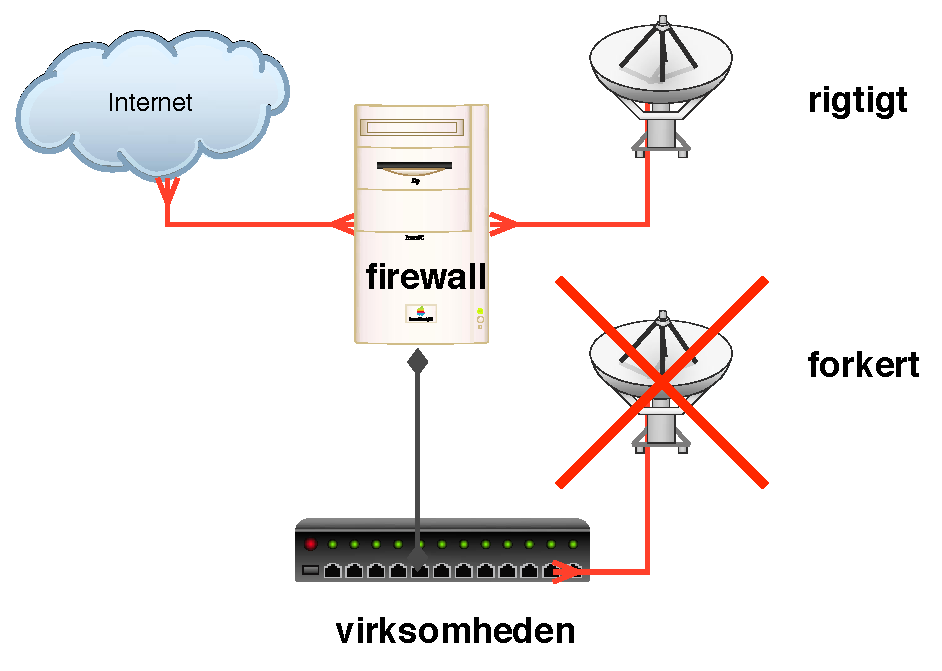
\includegraphics[height=11cm]{images/wlan-accesspoint-2.pdf}}
\end{center}

\centerline{\hlkbig S�dan b�r et access point forbindes til netv�rket}


\slide{Anbefalinger mht. tr�dl�se netv�rk}

\begin{minipage}{10cm}
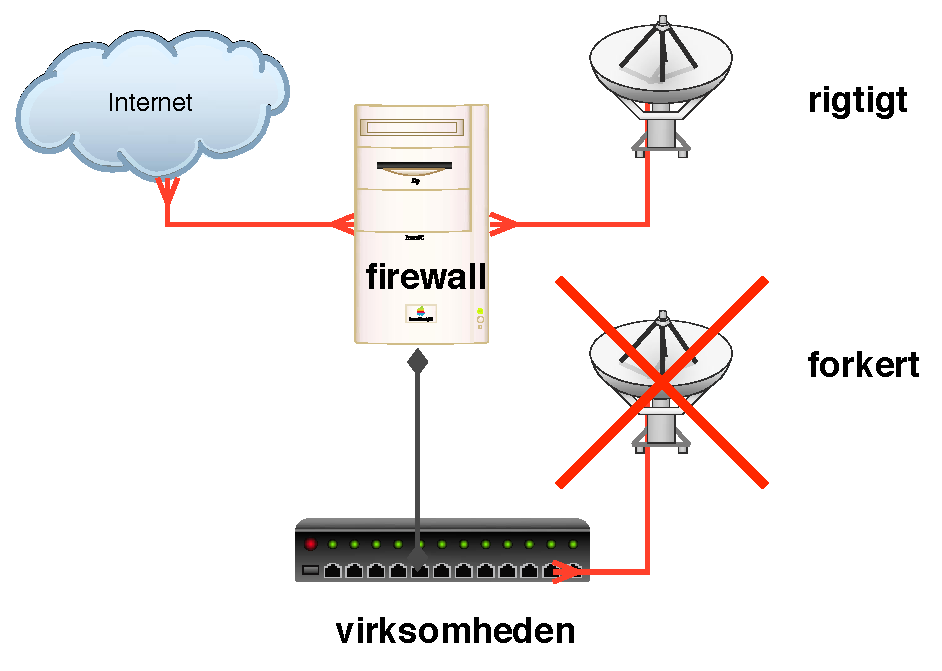
\includegraphics[width=10cm]{images/wlan-accesspoint-2.pdf}
\end{minipage}
\begin{minipage}{\linewidth-10cm}
\begin{list2}
\item Brug noget tilf�ldigt som SSID - netnavnet
\item Brug ikke WEP til virksomhedens netv�rk\\
- men istedet en VPN l�sning med individuel
  autentificering eller WPA
\item NB: WPA Personal/PSK kr�ver passphrase p� +40 tegn!
\item Placer de tr�dl�se adgangspunkter hensigtsm�ssigt i netv�rket -
  s� de kan overv�ges
\item Lav et s�t regler for brugen af tr�dl�se netv�rk - hvor m� 
  medarbejdere bruge det?
\item Se eventuelt pjecerne \emph{Beskyt dit tr�dl�se Netv�rk} fra
Ministeriet for Videnskab, Teknologi og Udvikling \\
\link{http://www.videnskabsministeriet.dk/}
\end{list2}
\end{minipage} 


\slide{Hjemmenetv�rk for n�rder}

\begin{list1}
\item Lad v�re med at bruge et wireless-kort i en PC til at lave AP, brug et AP
\item Husk et AP kan v�re en router, men den kan ofte ogs� blot v�re en bro
\item Brug WPA og overvej at lave en decideret DMZ til WLAN
\item Placer AP hensigtsm�ddigt og gerne h�jt, oppe p� et skab eller lignende
\end{list1}

%\exercise{ex:AirPort-AP}

%\exercise{ex:wardriving-windows}
%\exercise{ex:wardriving-kismet}
%\exercise{ex:aircrack-ng}
% 802.11 sikkerhed her



% RADIUS her

\slide{RADIUS}
\begin{list1}
\item RADIUS er en protokol til autentificering af brugere op mod en
  f�lles server 
\item Remote Authentication Dial In User Service (RADIUS)
\item RADIUS er beskrevet i RFC-2865
\item RADIUS kan v�re en fordel i st�rre netv�rk med 
\begin{list2}
\item dial-in
\item administration af netv�rksudstyr
\item tr�dl�se netv�rk
\item andre RADIUS kompatible applikationer
\end{list2}
\end{list1}

% LDAP her
\slide{LDAP}

\begin{list1}
\item LDAP er en protokol til directory access, opslag i database
\item Light udgave af den X.500 directory access standard 
\item LDAP er beskrevet i RFC-3377: Lightweight Directory Access Protocol 
(v3): Technical Specification
\item Standard interface for opslag, men desv�rre ikke for data
\item Bruges meget typisk til brugere, grupper og passwords
\end{list1}

\exercise{ex:radius-client}


\exercise{ex:ldap-client}


% 802.1x
\slide{IEEE 802.1x  Port Based Network Access Control}

\hlkimage{15cm}{osx-8021x.png}

\begin{list1}
\item Nogle switche tillader at man benytter 802.1x brugervalidering p� portniveau
\item Adgang til porten baseret p� brugernavn og kodeord/certifikat
\item Denne protokol indg�r ogs� i WPA Enterprise
\end{list1}


\slide{802.1x og andre teknologier}

\begin{list1}
\item 802.1x giver v�sentlige fordele
\item MAC filtrering kan spoofes, hvor 802.1x kr�ver det rigtige kodeord
\item WEP og WPA-PSK er een n�gle til alle brugere, 802.1x er individuel adgang
\item Typisk benyttes RADIUS integration mod LDAP eller Active Directory
\end{list1}


% netv�rksdesign her


\slide{Infrastrukturer i praksis}

\begin{list1}
\item Vi vil nu gennemg� netv�rksdesign med udgangspunkt i vores setup
\item Vores setup indeholder:
\begin{list2}
\item Routere
\item Firewall
\item Wireless
\item DMZ
\item DHCPD, BIND, BGPD, ...
\end{list2}
\item Den kunne udvides med flere andre teknologier vi har til r�dighed:
\begin{list2}
\item VLAN inkl VLAN trunking/distribution
\item WPA Enterprise
\end{list2}
\end{list1}



% VoIP her

\slide{VoIP Voice over IP}

\begin{list1}
\item Tidligere havde vi adskilte netv�rk, nu samles de 
\item Idag er det meget normalt at b�de firmaer og private bruger IP-telefoni
\item Fordele er prim�rt billigere og mere fleksibelt
\item Eksempler p� IP telefoni:
\begin{list2}
\item Skype benytter IP, men egenudviklet protokol
\item Cisco IP-telefoner benyttes ofte i firmaer
\item Cybercity telefoni k�rer over IP, med analog adapter
\end{list2}
\item Det anbefales at se p� Asterisk telefoniserver, hvis man har mod p� det :-)
\item \link{http://www.asterisk.org/}
\end{list1}

\slide{VoIP bekymringer}

\begin{list1}
\item Der er generelt problemer med:
\begin{list2}
\item Stabilitet - quality of service, netv�rket skal v�re bygget til det
\item Sikkerhed - hvem lytter med, hvem kan afbryde forbindelsen\\
Se evt. \link{http://www.voipsa.org/}
\item Spam over VoIP, connect, send WAV fil med spam kaldes SPIT
\item Kompatabilitet - hvilke protokoller, codecs, standarder, ...
\end{list2}
\item Der er flere store spillere
\end{list1}

\slide{VoIP protokoller}

\begin{list1}
\item SIP Session Initiation Protocol, IETF standard signaleringsprotokol
\item H.323 ITU-T standard signaleringsprotokol
\item IAX Inter-Asterisk Exchange Protocol, Asterisk protokol
\item SSCP Cisco protokol
\item ZRTP Phil Zimmermann, zfone - sikker kommunikation\\ 
\link{http://zfoneproject.com/}
\end{list1}

% efter VoIP

\slide{TFTP Trivial File Transfer Protocol}

\begin{list1}
\item Trivial File Transfer Protocol - uautentificerede filoverf�rsler
\item De bruges is�r til:
  \begin{list2}
\item TFTP bruges til boot af netv�rksklienter uden egen harddisk
\item TFTP benytter UDP og er derfor ikke garanteret at data overf�res korrekt
  \end{list2}
\item TFTP sender alt i klartekst, hverken password \\ 
\item FTP bruger TCP men sender ogs� i klartekst:
{\bfseries USER brugernavn} og \\
{\bfseries PASS hemmeligt-kodeord} 
\end{list1}

\slide{B�ndbreddestyring og policy based routing}

\begin{list1}
\item Mange routere og firewalls idag kan lave b�ndbredde allokering til
  protokoller, porte og derved bestemte services
\item Mest kendte er i Open Source:
\begin{list2}
\item ALTQ bruges p� OpenBSD - integreret i PF
%  \link{http://www.csl.sony.co.jp/person/kjc/kjc/software.html}
\item FreeBSD har dummynet
\item Linux har tilsvarende\\
ADSL-Bandwidth-Management-HOWTO, ADSL Bandwidth Management HOWTO\\
Adv-Routing-HOWTO, Linux Advanced Routing \& Traffic Control HOWTO\\
\link{http://www.knowplace.org/shaper/resources.html} Linux resources
\end{list2}
\item Det kaldes ogs� traffic shaping
\end{list1}

\slide{Firewalls - packet filtering}

\begin{alltt}
\small
0                   1                   2                   3   
0 1 2 3 4 5 6 7 8 9 0 1 2 3 4 5 6 7 8 9 0 1 2 3 4 5 6 7 8 9 0 1 
+-+-+-+-+-+-+-+-+-+-+-+-+-+-+-+-+-+-+-+-+-+-+-+-+-+-+-+-+-+-+-+-+
|Version|  IHL  |Type of Service|          Total Length         |
+-+-+-+-+-+-+-+-+-+-+-+-+-+-+-+-+-+-+-+-+-+-+-+-+-+-+-+-+-+-+-+-+
|         Identification        |Flags|      Fragment Offset    |
+-+-+-+-+-+-+-+-+-+-+-+-+-+-+-+-+-+-+-+-+-+-+-+-+-+-+-+-+-+-+-+-+
|  Time to Live |    Protocol   |         Header Checksum       |
+-+-+-+-+-+-+-+-+-+-+-+-+-+-+-+-+-+-+-+-+-+-+-+-+-+-+-+-+-+-+-+-+
|                       Source Address                          |
+-+-+-+-+-+-+-+-+-+-+-+-+-+-+-+-+-+-+-+-+-+-+-+-+-+-+-+-+-+-+-+-+
|                    Destination Address                        |
+-+-+-+-+-+-+-+-+-+-+-+-+-+-+-+-+-+-+-+-+-+-+-+-+-+-+-+-+-+-+-+-+
|                    Options                    |    Padding    |
+-+-+-+-+-+-+-+-+-+-+-+-+-+-+-+-+-+-+-+-+-+-+-+-+-+-+-+-+-+-+-+-+  
\end{alltt}

\begin{list1}
\item Packet filtering er firewalls der filtrerer p� IP niveau
\item Idag inkluderer de fleste statefull inspection 
\end{list1}

\slide{TCP three way handshake}

\hlkimage{7cm}{images/tcp-three-way.pdf}

\begin{list2}
\item Hvis en maskine modtager mange SYN pakker kan dette fylde
  tabellen over connections op - og derved afholde nye forbindelser
  fra at blive oprettet - {\bfseries SYN-flooding}
\item Mange firewalls kan udf�re SYN handshake idag, f�r forbindelsen overlades til serveren bagved
\item Beskytter mod {\bfseries TCP SYN flooding}
\end{list2}


\slide{Kommercielle firewalls}
\begin{list2}
\item Checkpoint Firewall-1 \link{http://www.checkpoint.com}
\item Nokia appliances - Nokia IPSO \link{http://www.nokia.com}
\item Cisco PIX \link{http://www.cisco.com}
\item Clavister firewalls \link{http://www.clavister.com}
\item Netscreen - nu ejet af Juniper
  \link{http://www.juniper.net}
\end{list2}

Ovenst�ende er dem som jeg oftest ser ude hos mine kunder

\slide{Open source baserede firewalls}
\begin{list2} 
\item Linux firewalls - fra begyndelsen til det nuv�rende netfilter
  til kerner version 2.4 og 2.6\\
\link{http://www.netfilter.org}
\item Firewall GUIs ovenp� Linux - mange! IPcop, Guarddog, Watchguard
nogle Linux firewalls er kommercielle produkter
\item IP Filter (IPF) \link{http://coombs.anu.edu.au/~avalon/}
\item OpenBSD PF - findes idag p� andre operativsystemer
\link{http://www.openbsd.org} 
\item FreeBSD IPFW og IPFW2 \link{http://www.freebsd.org}
\item FreeBSD inkluderer ogs� OpenBSD PF
\item Mac OS X benytter IPFW og har en application socket firewall
\item NetBSD - bruger IPF og OpenBSD PF
\end{list2}

NB: kun eksempler og dem jeg selv har brugt


\slide{Hardware eller software}


\begin{list1}
\item Man h�rer indimellem begrebet \emph{hardware firewall}  
\item Det er dog et faktum at en firewall best�r af:
\begin{list2}
\item Netv�rkskort - som er hardware
\item Filtreringssoftware - som er \emph{software}!    
\end{list2}
\item Det giver ikke mening at kalde en Zyxel 10 en hardware firewall
  og en Soekris med OpenBSD for en software firewall!
\item Det er efter min mening et marketingtrick
\vskip 1 cm
\item Man kan til geng�ld godt argumentere for at en dedikeret
  firewall som en separat enhed kan give bedre sikkerhed
\end{list1}



\slide{m0n0wall}

\hlkimage{20cm}{images/m0n0wall-1.pdf}

Kilde: billede fra \link{http://m0n0.ch/wall/}



\slide{firewall koncepter}

\begin{list1}
\item R�kkef�lgen af regler betyder noget!
\begin{list2}
\item To typer af firewalls:
 First match - n�r en regel matcher, g�r det som angives block/pass
 Last match  - marker pakken hvis den matcher, til sidst afg�res block/pass
\end{list2}
\item {\bf Det er ekstremt vigtigt at vide hvilken type firewall
    man bruger!} 
\item OpenBSD PF er last match
\item FreeBSD IPFW er first match  
\item Linux iptables/netfilter er last match
\end{list1}

\slide{First or Last match firewall?}

\hlkimage{20cm}{images/first-last-match-1.pdf}
\begin{list2}
\item To typer af firewalls:
 First match - eksempelvis IPFW,
 Last match - eksempelvis PF
%\item {\bf Det er ekstremt vigtigt at vide hvilken type firewall
%    man bruger!} 
\end{list2}


\slide{First match - IPFW}

\begin{alltt}
\hlksmall
00100 16389  1551541 allow ip from any to any via lo0
00200     0        0 deny log ip from any to 127.0.0.0/8
00300     0        0 check-state
...
{\bfseries 
65435    36     5697 deny log ip from any to any}
65535   865    54964 allow ip from any to any
\end{alltt}

\vskip 2 cm

\centerline{Den sidste regel n�s aldrig!}

\slide{Last match - OpenBSD PF}

\begin{alltt}
\small
ext_if="ext0"
int_if="int0"

block in
pass out keep state

pass quick on \{ lo $int_if \}

# Tillad forbindelser ind p� port 80=http og port 53=domain
# p� IP-adressen for eksterne netkort ($ext_if) syntaksen
pass in on $ext_if proto tcp to ($ext_if) port http keep state
pass in on $ext_if proto \{ tcp, udp \} to ($ext_if) port domain keep state
\end{alltt}

\vskip 2 cm
\centerline{Pakkerne markeres med block eller pass indtil sidste
  regel}
\centerline{n�gleordet \emph{quick} afslutter match - god til store
  regels�t} 


\slide{Firewalls og ICMP}


\begin{alltt}
ipfw add allow icmp from any to any icmptypes 3,4,11,12
\end{alltt}

\begin{list1}
\item Ovenst�ende er IPFW syntaks for at tillade de interessant ICMP beskeder igennem
\item Tillad ICMP types:
\begin{list2}
\item 3 Destination Unreachable
\item 4 Source Quench Message
\item 11 Time Exceeded
\item 12 Parameter Problem Message
\end{list2}
\end{list1}




\slide{netdesign - med firewalls - 100\% sikkerhed?}

\begin{center}
\colorbox{white}{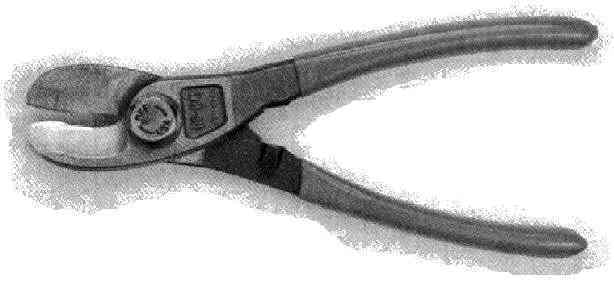
\includegraphics[width=12cm]{images/kut.jpg}}  
\end{center}

\begin{list1}
\item Hvor skal en firewall placeres for at g�re st�rst nytte?
\item Hvad er foruds�tningen for at en firewall virker?\\
At der er konfigureret et s�t fornuftige regler!
\item Hvor kommer reglerne fra? Sikkerhedspolitikken!
%\item Kan man lave en 100\% sikker firewall? Ja selvf�lgelig, se!
\end{list1}


\centerline{\small Kilde: Billedet er fra Marcus Ranum The ULTIMATELY
  Secure Firewall} 


\slide{Bloker indefra og ud}

\begin{list1}
\item Der er porte og services som altid b�r blokeres
\item Det kan v�re kendte s�rbare services
\begin{list2}
\item Windows SMB filesharing - ikke til brug p� Internet!
\item Unix NFS - ikke til brug p� Internet!
\end{list2}
\item Kendte problemer:
\begin{list2}
\item KaZaA og andre P2P programmer - hvis muligt!
\item Portmapper - port 111    
\end{list2}
\end{list1}


\slide{Firewall konfiguration}

\begin{list1}
\item Den bedste firewall konfiguration starter med:
\begin{list2}
\item Papir og blyant
\item En fornuftig adressestruktur
\end{list2}
\item Brug dern�st en firewall med GUI f�rste gang!
\item Husk dern�st:
\begin{list2}
\item En firewall skal passes
\item En firewall skal opdateres
\item Systemerne bagved skal h�rdes!    
\end{list2}
\end{list1}



\slide{Netv�rksdesign og sikkerhed}

\begin{list1}
\item Hvad kan man g�re for at f� bedre netv�rkssikkerhed?
\begin{list2}
\item Bruge switche - der skal ARP spoofes og bedre performance
\item Opdele med firewall til flere DMZ zoner for at holde
      udsatte servere adskilt fra hinanden, det interne netv�rk og
      Internet
\item Overv�ge, l�se logs og reagere p� h�ndelser 
\end{list2}
\item Husk du skal ogs� kunne opdatere dine servere
\end{list1}


\slide{En typisk firewall konfiguration}

\hlkimage{17cm}{images/firma-netvaerk.pdf}

\begin{list1}
\item Du b�r opdele dit netv�rk i segmenter efter traffik
\item Du b�r altid holde interne og eksterne systemer adskilt!
\item Du b�r isolere farlige services i jails og chroots
\end{list1}


\slide{Seperation of privileges} 

\begin{list1}
\item Forskellige computere til forskellige form�l, en server er mail-server en anden er web-server
\item Brug en sikker konfiguration, minimumskonfiguration
\item Brug sikre protokoller, kryptering SSH fremfor Telnet
\item Ops�tning af netv�rk, hvordan? Security Configuration Guides + paranoia
\begin{list2}
\item \link{http://csrc.nist.gov/publications/PubsSPs.html}
\item \link{http://www.nsa.gov/research/publications/index.shtml}
\item \link{http://www.nsa.gov/ia/guidance/security_configuration_guides/index.shtml}
\end{list2}
\end{list1}



\slide{Proxy servers}

\begin{list1}
\item Filtrering p� h�jere niveauer i OSI modellen er muligt
\item Idag findes proxy applikationer til de mest almindelige
  funktioner
\item Den typiske proxy er en caching webproxy der kan foretage HTTP
  request p� vegne af arbejdsstationer og gemme resultatet 
\item NB: nogle protokoller egner sig ikke til proxy servere
\item SSL forbindelser til \emph{secure websites} kan per design ikke proxies
\end{list1}

\slide{Unified communications}

\hlkimage{23cm}{firma-netvaerk-wlan}

\slide{Redundante firewalls}

\hlkimage{8cm}{images/pfsync-carp-1.jpg}

\begin{list2}
\item OpenBSD Common Address Redundancy Protocol CARP - b�de IPv4 og IPv6\\
overtagelse af adresse b�de IPv4 og IPv6
\item pfsync - sender opdateringer om firewall states mellem de to systemer  
\item Kilde:
\link{http://www.countersiege.com/doc/pfsync-carp/}
\end{list2}

\exercise{ex:unix-basic-firewall}
\exercise{ex:nmap-sweep}
\exercise{ex:nmap-portscan}

\slide{IPsec og Andre VPN features}

\begin{list1}
\item De fleste firewalls giver mulighed for at lave krypterede
  tunneler
\item Nyttigt til fjernkontorer der skal have usikker traffik henover
  usikre netv�rk som Internet 
\item Konceptet kaldes Virtual Private Network VPN
\item IPsec er de facto standarden for VPN og beskrevet i RFC'er 
\end{list1}

\slide{IPsec}

\begin{list1}
\item Sikkerhed i netv�rket
\begin{list2}
\item RFC-2401 Security Architecture for the Internet Protocol
\item RFC-2402 IP Authentication Header (AH)
\item RFC-2406 IP Encapsulating Security Payload (ESP)
\item RFC-2409 The Internet Key Exchange (IKE) - dynamisk keying
\end{list2}
\item B�de til IPv4 og IPv6
\item {\bfseries MANDATORY} i IPv6! - et krav hvis man implementerer
  fuld IPv6 support
\item Der findes IKEscan til at scanne efter IKE
  porte/implementationer\\
\link{http://www.nta-monitor.com/ike-scan/index.htm}
\end{list1}

\slide{IPsec er ikke simpelt!}

\hlkimage{16cm}{images/ipsec-hsc.png}
\centerline{Kilde: \link{http://www.hsc.fr/presentations/ike/}}



\slide{RFC-2406 IP ESP}

Pakkerne f�r og efter:
\begin{alltt}
\small 
               BEFORE APPLYING ESP
         ---------------------------------------
   IPv6  |             | ext hdrs |     |      |
         | orig IP hdr |if present| TCP | Data |
         ---------------------------------------



               AFTER APPLYING ESP
         ---------------------------------------------------------
   IPv6  | orig |hop-by-hop,dest*,|   |dest|   |    | ESP   | ESP|
         |IP hdr|routing,fragment.|ESP|opt*|TCP|Data|Trailer|Auth|
         ---------------------------------------------------------
                                   |<---- encrypted ---->|
                               |<---- authenticated ---->| 
\end{alltt}


\slide{OpenVPN / OpenSSL VPN}

\begin{quote}
OpenVPN is a full-featured SSL VPN solution which can accomodate a
wide range of configurations, including remote access, site-to-site
VPNs, WiFi security, and enterprise-scale remote access solutions with
load balancing, failover, and fine-grained access-controls (articles)
(examples) (security overview) (non-english languages).   
\end{quote}

\begin{list1}
\item Et andet popul�rt VPN produkt er OpenVPN
\item Bem�rk dog at hvis der benyttes TCP i TCP risikerer man at st�de ind i 
et problem som kaldes \emph{TCP in TCP meltdown} 
\item Kilde: \link{http://openvpn.net/}  
\end{list1}


\slide{Network patterns }

\begin{list1}
\item Hvad taler for og imod - de n�ste slides gennemg�r nogle standardsetups
\item En slags Patterns for networking
\end{list1}

 
\slide{Pattern: erstat Telnet med SSH}

\begin{list1}
\item Telnet er d�d!
\item Brug altid Secure Shell fremfor Telnet
\item Opgrader firmware til en der kan SSH, eller k�b bedre udstyr n�ste gang
\item Selv mine sm� billige Linksys switche forst�r SSH!
\end{list1}

\slide{Pattern: erstat FTP med HTTP}

\begin{list1}
\item Hvis der kun skal distribueres filer kan man ofte benytte HTTP istedet for FTP
\item Hvis der skal overf�res med password er SCP/SFTP fra Secure Shell at foretr�kke
\end{list1}


\slide{Anti-patterns}

\begin{list1}
\item Nu pr�senteres et antal setups, som ikke anbefales
\item Faktisk vil jeg advare mod at bruge dem
\item Husk f�lgende slides er min mening
\end{list1}

\slide{Anti-pattern dobbelt NAT i eget netv�rk}

\hlkimage{20cm}{nat-double.pdf}

\begin{list1}
\item Det er n�dvendigt med NAT for at overs�tte traffik der sendes videre
ud p� internet.
\vskip 1cm
\item Der er ingen som helst grund til at benytte NAT indenfor eget netv�rk!
\end{list1}

\slide{Anti-pattern blokering af ALT ICMP}

\begin{alltt}
ipfw add allow icmp from any to any icmptypes 3,4,11,12
\end{alltt}

\begin{list1}
\item Lad v�re med at blokere for alt ICMP, s� �del�gger du funktionaliteten i dit net 
\vskip 1cm
\item \end{list1}

\slide{Anti-pattern blokering af DNS opslag p� TCP}

\begin{list1}
\item Det bliver (er) n�dvendigt med DNS opslag over TCP p� grund af store svar. Det betyder at firewalls skal tillade DNS opslag via TCP
\vskip 1cm
\item 
\item Guide:\\
Brug en caching nameserver, s�ledes at det kun er den som kan lave DNS opslag ud i verden

\end{list1}

\slide{Anti-pattern daisy-chain}

\hlkimage{20cm}{daisy-chain-server.pdf}

\begin{list1}
\item Daisy-chain af servere, erstat med firewall, switch og VLAN
\vskip 1cm
\item Det giver et v�ld af problemer med overv�gning, administration, backup og opdatering
\end{list1}

\slide{Anti-pattern WLAN forbundet direkte til LAN}

\hlkimage{10cm}{images/wlan-accesspoint-2.pdf}

\begin{list1}
\item WLAN AP'er forbundet direkte til LAN giver st�rre risiko for at sikkerheden brydes
\item Ved at s�tte WLAN direkte p� LAN risikerer man at eksterne f�r direkte adgang
\item Kan selvf�lgelig g� an i et privat hjem
\item Det forv�rres jo flere AP'er man har, har du 100 skal du v�re sikker p� allesammen er sikre!
\end{list1}







\slide{Dag 3 Dynamiske protokoller og services}

\hlkimage{20cm}{openbgpd-network-2.pdf}

% 802.11 start
%input fra wireless kursus, wireless pr�sentationer, wireless foredrag pentest III
%Husk WDS og bridging

\slide{Tr�dl�se teknologier 802.11}

\begin{list1}
\item 802.11 er arbejdsgruppen under IEEE 
\item De mest kendte standarder idag indenfor tr�dl�se teknologier:
\begin{list2}
\item 802.11b 11Mbps versionen
\item 802.11g 54Mbps versionen
\item 802.11n endnu hurtigere, og draft
\item 802.11i Security enhancements
\end{list2}
\item Der er propriet�re versioner 22Mbps og den slags\\
- det anbefales IKKE at benytte disse da det giver vendor lock-in -
man bliver l�st fast
\end{list1}

Kilde: \link{http://grouper.ieee.org/groups/802/11/index.html}

\slide{802.11 modes og frekvenser}

\begin{list1}
\item Access point k�rer typisk i \emph{access point mode} ogs� kaldet
  infrastructure mode - al trafik g�r via AP
\item Alternativt kan wireless kort oprette ad-hoc netv�rk - hvor
  trafikken g�r direkte mellem netkort
\item Frekvenser op til kanal 11 og 12+13 i DK/EU
\item Helst 2 kanaler spring for 802.11b AP der placeres indenfor r�kkevidde
\item Helst 4 kanaler spring for 802.11g AP der placeres indenfor r�kkevidde
\end{list1}

\slide{Eksempel p� netv�rk med flere AP'er}

\hlkimage{20cm}{images/wireless-multi-ap.pdf}

\slide{Eksempel p� netv�rk med flere AP'er}

\hlkimage{20cm}{images/wireless-multi-ap-2.pdf}


\slide{Wireless Distribution System WDS}

\hlkimage{18cm}{images/wireless-multi-ap-wds.pdf}

\begin{list1}
\item Se ogs�:
\link{http://en.wikipedia.org/wiki/Wireless_Distribution_System}
\end{list1}


\slide{\hskip 1 cm Er tr�dl�se netv�rk interessante?}

\begin{list1}
\item Sikkerhedsproblemer i de tr�dl�se netv�rk er mange
  \begin{list2}
  \item Fra lavt niveau - eksempelvis ARP, 802.11
  \item d�rlige sikringsmekanismer - WEP
  \item d�rligt udstyr - mange fejl
  \item usikkkerhed om implementering og overv�gning
  \end{list2}
\item Tr�dl�st udstyr er blevet meget billigt!
\item Det er et krav fra brugerne - tr�dl�st er l�kkert
\end{list1}


\slide{Konsekvenserne}

\hlkimage{10cm}{images/wireless-daekning.pdf}

\begin{list2}
\item V�rre end Internetangreb - anonymt
\item Kr�ver ikke fysisk adgang til lokationer
%\emph{spioneres imod}
\item Konsekvenserne ved sikkerhedsbrud er generelt st�rre
\item Typisk f�r man direkte LAN eller Internet adgang!
\end{list2}

\slide{V�rkt�jer}

\begin{list1}
\item Alle bruger nogenlunde de samme v�rkt�jer, m�ske forskellige
  m�rker
\begin{list2}
\item Wirelessscanner - Kismet og netstumbler
\item Wireless Injection - typisk p� Linux
\item ...
\item Aircrack-ng
\end{list2}
\item Jeg anbefaler Auditor Security Collection og BackTrack boot CD'erne
\end{list1}


\slide{Konsulentens udstyr wireless}

\begin{list1}
\item Laptop med PC-CARD slot
\item Tr�dl�se kort Atheros, de indbyggede er ofte ringe ;-)
\item Access Points - jeg anbefaler Airport Express
\item Antenner hvis man har lyst
\item B�ger: 
\begin{list2}
\item \emph{Real 802.11 security}
\item Se oversigter over b�ger og v�rkt�jer igennem pr�sentationen:
\end{list2}
\item Internetressourcer:
\begin{list2}
\item BackTrack - CD image med Linux+v�rkt�jer    
\item Packetstorm wireless tools
\link{http://packetstormsecurity.org/wireless/}
\item \emph{Beginner's Guide to Wireless Auditing}
David Maynor 
\link{http://www.securityfocus.com/infocus/1877?ref=rss}
\end{list2}
\end{list1}


\slide{Typisk brug af 802.11 udstyr}

\begin{center}
\colorbox{white}{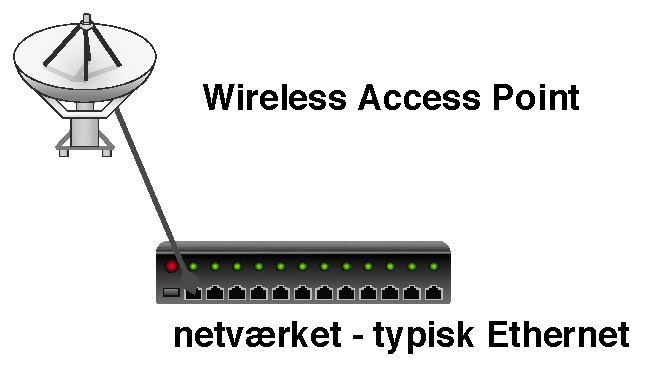
\includegraphics[width=20cm]{images/wlan-accesspoint-1.pdf}}
\end{center}

\centerline{\hlkbig et access point - forbindes til netv�rket}

\slide{Basal konfiguration}

\begin{list1}
\item N�r man tager fat p� udstyr til tr�dl�se netv�rk opdager man:
\item SSID - nettet skal have et navn
\item frekvens / kanal - man skal v�lge en kanal, eller udstyret
  v�lger en automatisk
\item der er nogle forskellige metoder til sikkerhed  
\end{list1}

\slide{Tr�dl�s sikkerhed}

\hlkimage{14cm}{images/apple-wireless-security.png}

\begin{list2}
\item Tr�dl�s sikkerhed - WPA og WPA2
\item Nem konfiguration
\item Nem konfiguration af Access Point  
\end{list2}

\slide{Wireless networking sikkerhed i 802.11b}

\hlkimage{10cm}{images/wlan-accesspoint-1.pdf}

\begin{list1}
\item Sikkerheden er baseret p� nogle f� foruds�tninger 
  \begin{list2}
  \item SSID - netnavnet
  \item WEP \emph{kryptering} - Wired Equivalent Privacy
  \item m�ske MAC flitrering, kun bestemte kort m� tilg� accesspoint 
  \end{list2}
\item Til geng�ld er disse foruds�tninger ofte ikke tilstr�kkelige ... 
%\item Hvorfor hader du WEP?
  \begin{list2}
  \item WEP er m�ske \emph{ok} til visse sm� hjemmenetv�rk
  \item WEP er baseret p� en DELT hemmelighed som alle stationer kender
  \item n�glen �ndres sj�ldent, og det er sv�rt at distribuere en ny
  \end{list2}
  
\end{list1}


\slide{Foruds�tninger}

\begin{list1}
\item Til geng�ld er disse foruds�tninger ofte ikke tilstr�kkelige ... 
\item Hvad skal man beskytte?
\item Hvordan kan sikkerheden omg�s?
\item Mange firmaer og virksomheder stille forskellige krav til
  sikkerheden - der er ikke en sikkerhedsmekanisme der passer til alle
\end{list1}

\slide{SSID - netnavnet}

\begin{list1}
\item Service Set Identifier (SSID) - netnavnet
\item 32 ASCII tegn eller 64 hexadecimale cifre
\item Udstyr leveres typisk med et standard netnavn
\begin{list2}
\item Cisco - tsunami
\item Linksys udstyr - linksys
\item Apple Airport, 3Com m.fl. - det er nemt at genkende dem  
\end{list2}
\item SSID kaldes ogs� for NWID - network id
\item SSID broadcast - udstyr leveres oftest med broadcast af SSID
\end{list1}


%wardriving her
\slide{Demo: wardriving med stumbler programmer}

\hlkimage{17cm}{images/macstumbler.png}  

\begin{list1}
\item man tager et tr�dl�st netkort og en b�rbar computer og noget software:
\begin{list2}
\item Netstumbler - Windows \link{http://www.netstumbler.com}
\item dstumbler - UNIX \link{http://www.dachb0den.com/projects/dstumbler.html}
\item iStumbler - Mac \link{http://www.istumbler.net/}
\item Kismet ... mange andre
  \end{list2}
\end{list1}

\slide{Start p� demo - wardriving}

\hlkimage{15cm}{images/server-client-wlan.pdf}

\begin{list2}
\item Almindelige laptops bruges til demo
\item Der startes et \emph{access point}
\end{list2}

\slide{MAC filtrering}

\begin{list1}
\item De fleste netkort tillader at man udskifter sin MAC adresse
\item MAC adressen p� kortene er med i alle pakker der sendes
\item MAC adressen er aldrig krypteret, for hvordan skulle pakken s�
  n� frem?
\item MAC adressen kan derfor overtages, n�r en af de tilladte
  stationer forlader omr�det ...
\end{list1}

\slide{Resultater af wardriving}

\begin{list1}
\item Hvad opdager man ved wardriving?
\begin{list2}
\item at WEP IKKE krypterer hele pakken
\item at alle pakker indeholder MAC adressen
\item WEP n�glen skifter sj�ldent
\item ca. 2/3 af de netv�rk man finder har ikke WEP sl�et til - og der
  er fri og uhindret adgang til Internet
\end{list2}
\item {\color{red}
Man kan alts� lytte med p� et netv�rk med WEP, genbruge en anden
maskines MAC adresse - og m�ske endda bryde WEP krypteringen.}
\item 
Medmindre man kender virksomheden og WEP n�glen ikke er skiftet ...
det er besv�rligt at skifte den, idet alle stationer skal opdateres.
\end{list1}

\slide{Stork�benhavn}

\begin{center}
\colorbox{white}{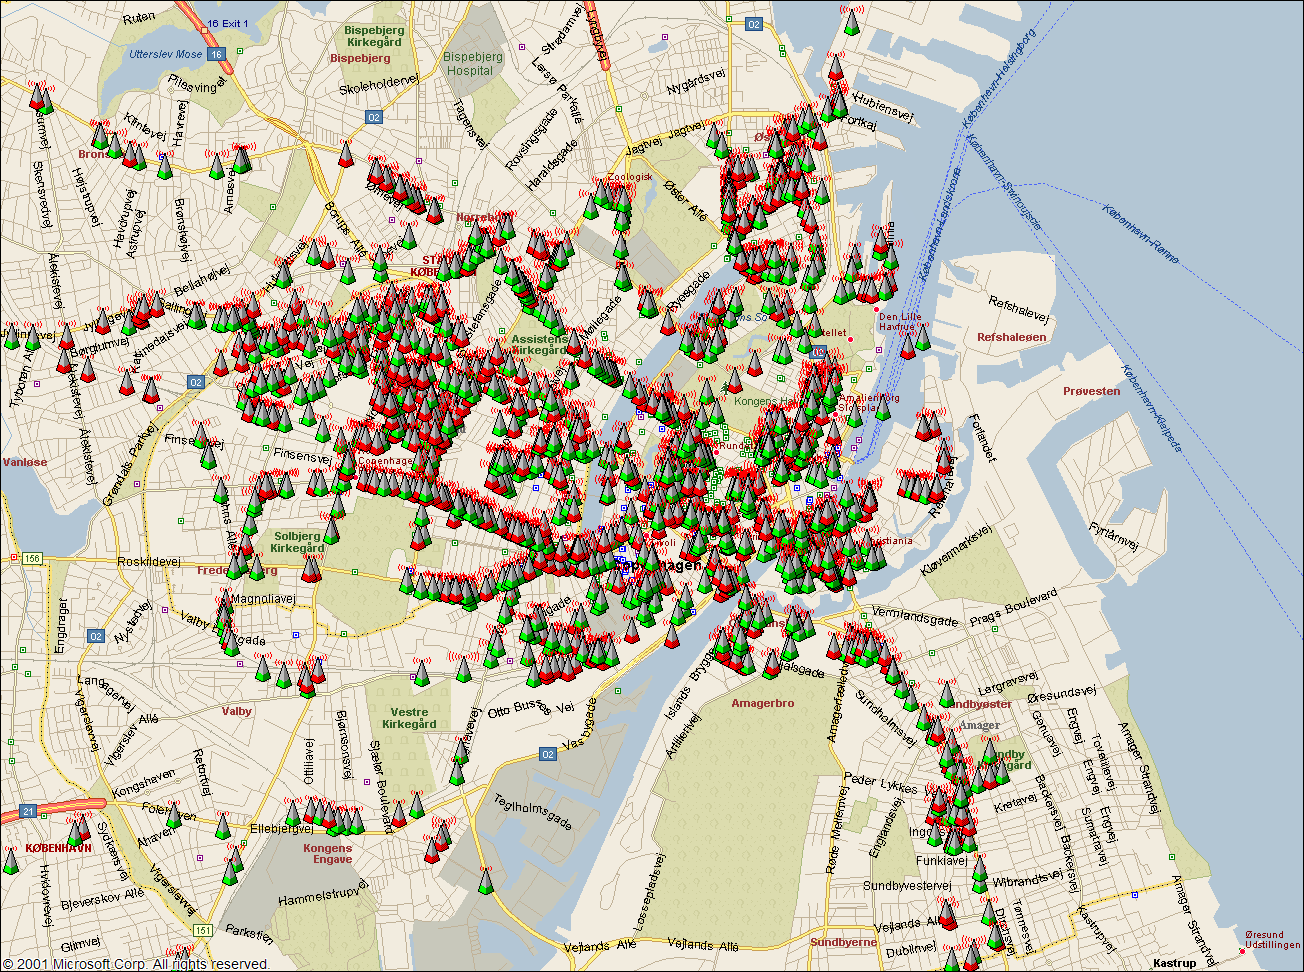
\includegraphics[width=20cm]{images/20030830-kbh.png}}  
\end{center}



\slide{Informationsindsamling}

\begin{list1}
\item Det vi har udf�rt er informationsindsamling
\item Indsamlingen kan v�re aktiv eller passiv indsamling i forhold
  til m�let for angrebet
\item passiv kunne v�re at lytte med p� trafik eller s�ge i databaser
  p� Internet
\item aktiv indsamling er eksempelvis at sende ICMP pakker og
  registrere hvad man f�r af svar
\end{list1}

\slide{WEP kryptering} 

%\begin{center}
%\colorbox{white}{
\includegraphics[width=12cm]{images/airsnort.pdf}}  
%\end{center}
\begin{list1}
\item WEP \emph{kryptering} - med n�gler der specificeres som tekst
  eller hexadecimale cifre
\item typisk 40-bit, svarende til 5 ASCII tegn eller 10 hexadecimale
  cifre eller 104-bit 13 ASCII tegn eller 26 hexadecimale cifre
\item WEP er baseret p� RC4 algoritmen der er en \emph{stream cipher}
  lavet af Ron Rivest for RSA Data Security
\end{list1}


\slide{De f�rste fejl ved WEP}
\begin{list1}
\item Oprindeligt en d�rlig implementation i mange Access Points
\item Fejl i krypteringen - rettet i nyere firmware
\item WEP er baseret p� en DELT hemmelighed som alle stationer kender
\item N�glen �ndres sj�ldent, og det er sv�rt at distribuere en ny
\end{list1}

\slide{WEP som sikkerhed}

\hlkimage{6cm}{images/no-wep.pdf}
\begin{list1}
\item WEP er \emph{ok} til et privat hjemmenetv�rk
\item WEP er for simpel til et st�rre netv�rk - eksempelvis 20 brugere
\item Firmaer b�r efter min mening bruge andre
  sikkerhedsforanstaltninger 
\item Hvordan udelukker man en bestemt bruger?
\end{list1}

\slide{WEP sikkerhed}

\hlkimage{12cm}{images/airsnort.pdf}  

\begin{quote}
AirSnort is a wireless LAN (WLAN) tool which recovers encryption
keys. AirSnort operates by passively monitoring transmissions,
computing the encryption key when enough packets have been gathered.  

802.11b, using the Wired Equivalent Protocol (WEP), is crippled with
numerous security flaws. Most damning of these is the weakness
described in " Weaknesses in the Key Scheduling Algorithm of RC4 "
by Scott Fluhrer, Itsik Mantin and Adi Shamir. Adam Stubblefield
was the first to implement this attack, but he has not made his
software public. AirSnort, along with WEPCrack, which was released
about the same time as AirSnort, are the first publicly available
implementaions of this attack.  \link{http://airsnort.shmoo.com/}
\end{quote}

%\begin{list1}
%\item i dag er firmware opdateret hos de fleste producenter
%\item men sikkerheden baseres stadig p� een delt hemmelighed
%\end{list1}

\slide{major cryptographic errors}

\begin{list1}
\item weak keying - 24 bit er allerede kendt - 128-bit = 104 bit i praksis
\item small IV - med kun 24 bit vil hver IV blive genbrugt oftere
\item CRC-32 som intergritetscheck er ikke \emph{st�rkt} nok
  kryptografisk set
\item Authentication gives pad - giver fuld adgang - hvis der bare
  opdages \emph{encryption pad} for en bestemt IV. Denne IV kan s�
  bruges til al fremtidig kommunikation
\end{list1}

{\hlkbig Konklusion: Kryptografi er sv�rt}

\slide{WEP cracking - airodump og aircrack}

\hlkimage{3cm}{images/no-wep.pdf}

\begin{list1}
\item airodump - opsamling af krypterede pakker
\item aircrack - statistisk analyse og fors�g p� at finde WEP n�glen
\item Med disse v�rkt�jer er det muligt at kn�kke \emph{128-bit n�gler}!
\item Blandt andet fordi det reelt er 104-bit n�gler \smiley
\item tommelfingerregel - der skal opsamles mange pakker ca. 500.000
  er godt
\item Links:\\
\link{http://www.cr0.net:8040/code/network/aircrack/} aircrack\\
\link{http://www.securityfocus.com/infocus/1814} WEP: Dead Again
\end{list1}

\slide{airodump afvikling}

\begin{list1}
\item N�r airodump k�rer opsamles pakkerne
\item samtidig vises antal initialisationsvektorer IV's:
\end{list1}

\vskip 1 cm

\begin{alltt}
\hlktiny
   BSSID              CH  MB  ENC  PWR  Packets   LAN IP / # IVs   ESSID

   00:03:93:ED:DD:8D   6  11       209   {\bf 801963                  540180}   wanlan    
\end{alltt}

\vskip 2 cm

\begin{list1}
\item NB: dataopsamlingen er foretaget p� 100\% opdateret Mac udstyr
\end{list1}


\slide{aircrack - WEP cracker}

\begin{alltt}
\hlktiny
   $ aircrack -n 128 -f 2 aftendump-128.cap
                                 aircrack 2.1
   * Got  540196! unique IVs | fudge factor = 2
   * Elapsed time [00:00:22] | tried 12 keys at 32 k/m
   KB    depth   votes
    0    0/  1   CE(  45) A1(  20) 7E(  15) 98(  15) 72(  12) 82(  12) 
    1    0/  2   62(  43) 1D(  24) 29(  15) 67(  13) 94(  13) F7(  13) 
    2    0/  1   B6( 499) E7(  18) 8F(  15) 14(  13) 1D(  12) E5(  10) 
    3    0/  1   4E( 157) EE(  40) 29(  39) 15(  30) 7D(  28) 61(  20) 
    4    0/  1   93( 136) B1(  28) 0C(  15) 28(  15) 76(  15) D6(  15) 
    5    0/  2   E1(  75) CC(  45) 39(  31) 3B(  30) 4F(  16) 49(  13) 
    6    0/  2   3B(  65) 51(  42) 2D(  24) 14(  21) 5E(  15) FC(  15) 
    7    0/  2   6A( 144) 0C(  96) CF(  34) 14(  33) 16(  33) 18(  27) 
    8    0/  1   3A( 152) 73(  41) 97(  35) 57(  28) 5A(  27) 9D(  27) 
    9    0/  1   F1(  93) 2D(  45) 51(  29) 57(  27) 59(  27) 16(  26) 
   10    2/  3   5B(  40) 53(  30) 59(  24) 2D(  15) 67(  15) 71(  12) 
   11    0/  2   F5(  53) C6(  51) F0(  21) FB(  21) 17(  15) 77(  15) 
   12    0/  2   E6(  88) F7(  81) D3(  36) E2(  32) E1(  29) D8(  27) 
         {\color{red}\bf KEY FOUND! [ CE62B64E93E13B6A3AF15BF5E6 ]}
\end{alltt}
%$


\slide{Hvor lang tid tager det?}

\begin{list1}
\item Opsamling a data - ca. en halv time p� 802.11b ved optimale forhold
\item Tiden for k�rsel af aircrack fra auditor CD 
p� en Dell CPi 366MHz Pentium II laptop:
\end{list1}
\begin{alltt}

   $ time aircrack -n 128 -f 2 aftendump-128.cap
   ...
   real    5m44.180s   user  0m5.902s     sys  1m42.745s
   \end{alltt}
   %$

\pause
\begin{list1}
\item Tiden for k�rsel af aircrack p� en moderne 1.6GHz CPU med
  almindelig laptop disk tager typisk mindre end 60 sekunder
\end{list1}

\slide{Erstatning for WEP- WPA}

\begin{list1}
\item Det anbefales at bruge:
%\begin{list2}
\item Kendte VPN teknologier eller WPA
\item baseret p� trov�rdige algoritmer
\item implementeret i professionelt udstyr
\item fra trov�rdige leverand�rer
\item udstyr der vedligeholdes og opdateres
%\end{list2}
\item Man kan m�ske endda bruge de eksisterende l�sninger - fra
  hjemmepc adgang, mobil adgang m.v.
\end{list1}


\slide{RADIUS}
\begin{list1}
\item RADIUS er en protokol til autentificering af brugere op mod en
  f�lles server 
\item Remote Authentication Dial In User Service (RADIUS)
\item RADIUS er beskrevet i RFC-2865
\item RADIUS kan v�re en fordel i st�rre netv�rk med 
\begin{list2}
\item dial-in
\item administration af netv�rksudstyr
\item tr�dl�se netv�rk
\item andre RADIUS kompatible applikationer
\end{list2}
\end{list1}


\slide{Erstatninger for WEP}
\begin{list1}
\item Der findes idag andre metoder til sikring af tr�dl�se netv�rk
\item 802.1x Port Based Network Access Control 
\item WPA - Wi-Fi Protected Access)\\
WPA = 802.1X + EAP + TKIP + MIC
\item nu WPA2
\begin{quote}
WPA2 is based on the final IEEE 802.11i amendment to the 802.11
standard and is eligible for FIPS 140-2 compliance.
\end{quote}
\item Kilde: 
\href{http://www.wifialliance.org/OpenSection/protected_access.asp}
{http://www.wifialliance.org/OpenSection/protected\_access.asp}
\end{list1}

\slide{WPA eller WPA2?}

\begin{quote}
WPA2 is based upon the Institute for Electrical and Electronics
Engineers (IEEE) 802.11i amendment to the 802.11 standard, which was
ratified on July 29, 2004.  
\end{quote}

\begin{quote}
Q: How are WPA and WPA2 similar?\\
A: Both WPA and WPA2 offer a high level of assurance for end-users and network
administrators that their data will remain private and access to their
network restricted to authorized users.
Both utilize 802.1X and Extensible Authentication Protocol (EAP) for
authentication. Both have Personal and Enterprise modes of operation
that meet the distinct needs of the two different consumer and
enterprise market segments. 

Q: How are WPA and WPA2 different?\\
A: WPA2 provides a {\bf stronger encryption mechanism} through {\bf
  Advanced Encryption Standard (AES)}, which is a requirement for some
corporate and government users. 
\end{quote}

\centerline{Kilde: http://www.wifialliance.org WPA2 Q and A}

\slide{WPA Personal eller Enterprise}

\begin{list1}
\item Personal - en delt hemmelighed, preshared key
\item Enterprise - brugere valideres op mod f�lles server
\item Hvorfor er det bedre?
\begin{list2}
\item Flere valgmuligheder - passer til store og sm�
\item WPA skifter den faktiske krypteringsn�gle j�vnligt - TKIP 
\item Initialisationsvektoren (IV) fordobles 24 til 48 bit   
\item Im�dekommer alle kendte problemer med WEP!
\item Integrerer godt med andre teknologier - RADIUS

\vskip 1 cm
\item EAP - Extensible Authentication Protocol - individuel autentifikation
\item TKIP - Temporal Key Integrity Protocol - n�gleskift og integritet
\item MIC - Message Integrity Code - Michael, ny algoritme til integritet
\end{list2}

\end{list1}


\slide{WPA cracking}

\begin{list1}
\item Nu skifter vi s� til WPA og alt er vel s� godt?  
\pause
\item Desv�rre ikke!
\item Du skal v�lge en laaaaang passphrase, ellers kan man sniffe WPA
  handshake n�r en computer g�r ind p� netv�rket!
\item Med et handshake kan man med aircrack igen lave off-line
  bruteforce angreb!
\end{list1}

\slide{WPA cracking demo}

\begin{list1}
\item Vi konfigurerer AP med Henrik42 som WPA-PSK/passhrase  
\item Vi finder netv�rk kismet eller airodump
\item Vi starter airodump mod specifik kanal
\item Vi spoofer deauth og opsamler WPA handshake
\item Vi kn�kker WPA :-)
\end{list1}

\centerline{Brug manualsiderne for programmerne i aircrack-ng pakken!}

\slide{WPA cracking med aircrack - start}

\begin{alltt}
\small
slax ~ # aircrack-ng -w dict wlan-test.cap
Opening wlan-test.cap
Read 1082 packets.

#  BSSID              ESSID           Encryption

1  00:11:24:0C:DF:97  wlan            WPA (1 handshake)
2  00:13:5F:26:68:D0  Noea            No data - WEP or WPA
3  00:13:5F:26:64:80  Noea            No data - WEP or WPA
4  00:00:00:00:00:00                  Unknown

Index number of target network ? {\bf 1}
\end{alltt}

\slide{WPA cracking med aircrack - start}

\begin{alltt}
\small
          [00:00:00] 0 keys tested (0.00 k/s)

                    KEY FOUND! [ Henrik42 ]

Master Key     : 8E 61 AB A2 C5 25 4D 3F 4B 33 E6 AD 2D 55 6F 76
                 6E 88 AC DA EF A3 DE 30 AF D8 99 DB F5 8F 4D BD
Transcient Key : C5 BB 27 DE EA 34 8F E4 81 E7 AA 52 C7 B4 F4 56
                 F2 FC 30 B4 66 99 26 35 08 52 98 26 AE 49 5E D7
                 9F 28 98 AF 02 CA 29 8A 53 11 EB 24 0C B0 1A 0D
                 64 75 72 BF 8D AA 17 8B 9D 94 A9 31 DC FB 0C ED

EAPOL HMAC     : 27 4E 6D 90 55 8F 0C EB E1 AE C8 93 E6 AC A5 1F

\end{alltt}

\vskip 1 cm

\centerline{Min Thinkpad X31 med 1.6GHz Pentium M kn�kker ca. 150 Keys/sekund}

\slide{Tools man b�r kende}

\begin{list2}
\item BSD Airtools \link{http://www.dachb0den.com/projects/bsd-airtools.html}
\item Kismet \link{http://www.kismetwireless.net/}
\item Airsnort \link{http://airsnort.shmoo.com/} l�s pakkerne med WEP
  kryptering  
\item wepcrack \link{http://wepcrack.sourceforge.net/} - kn�k
  krypteringen i WEP
\item Airsnarf \link{http://airsnarf.shmoo.com/} - lav dit eget AP
  parallelt med det rigtige og snif hemmeligheder
\item Wireless Scanner \link{http://www.iss.net/} - kommercielt 
\item Dette er et lille uddrag af programmer\\
Se ogs� \link{http://packetstormsecurity.org/wireless/}
\end{list2}

\slide{N�r adgangen er skabt}

\begin{list1}
\item S� g�r man igang med de almindelige v�rkt�jer
\item Fyodor Top 100 Network Security Tools \link{http://www.sectools.org}  
\end{list1}
\vskip 2 cm

\centerline{\hlkbig Forsvaret er som altid - flere lag af sikkerhed! }

\slide{Infrastruktur�ndringer}

\begin{center}
\colorbox{white}{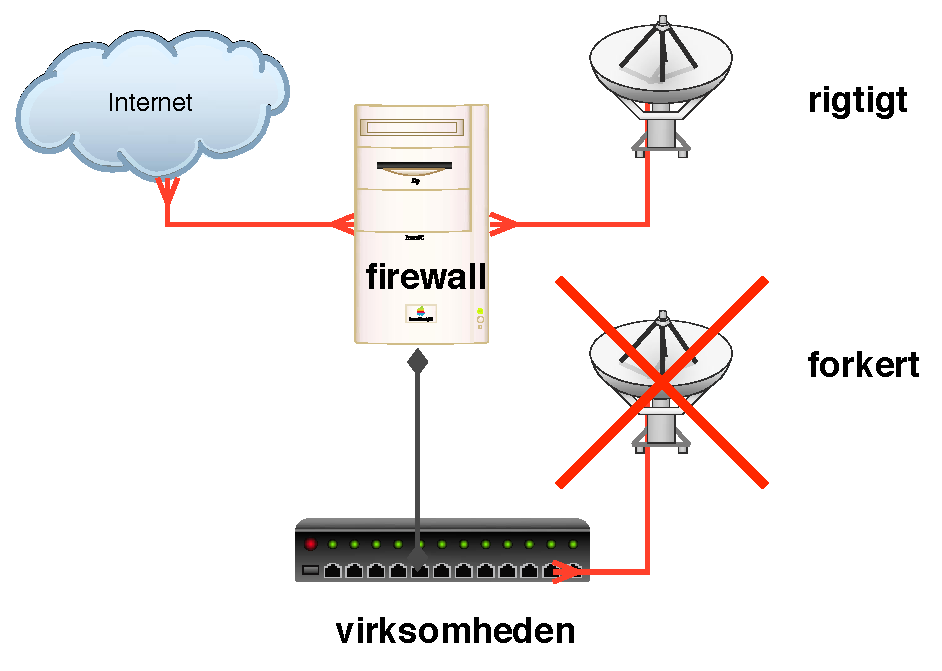
\includegraphics[height=11cm]{images/wlan-accesspoint-2.pdf}}
\end{center}

\centerline{\hlkbig S�dan b�r et access point forbindes til netv�rket}


\slide{Anbefalinger mht. tr�dl�se netv�rk}

\begin{minipage}{10cm}
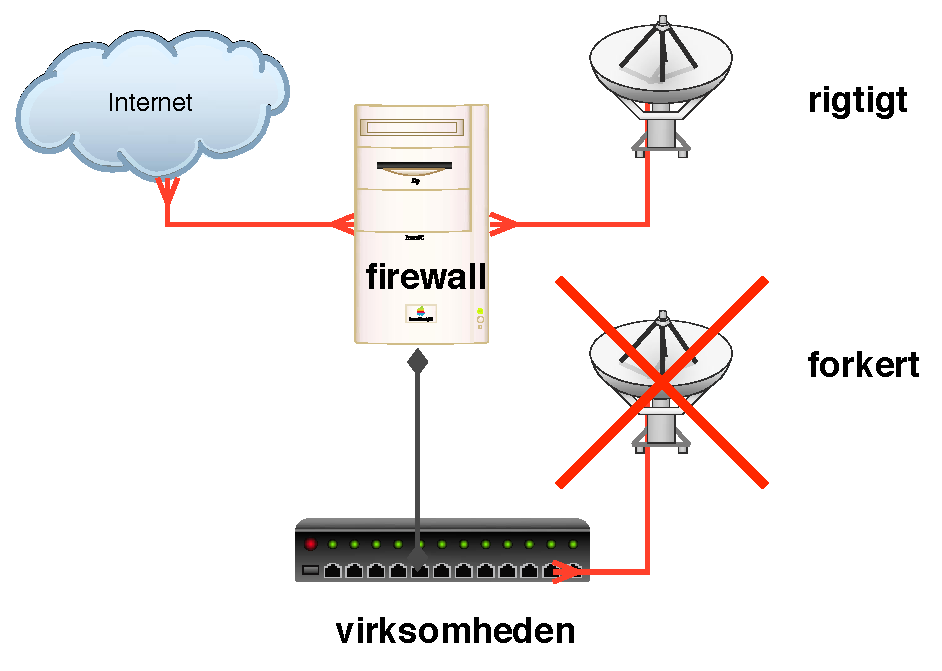
\includegraphics[width=10cm]{images/wlan-accesspoint-2.pdf}
\end{minipage}
\begin{minipage}{\linewidth-10cm}
\begin{list2}
\item Brug noget tilf�ldigt som SSID - netnavnet
\item Brug ikke WEP til virksomhedens netv�rk\\
- men istedet en VPN l�sning med individuel
  autentificering eller WPA
\item NB: WPA Personal/PSK kr�ver passphrase p� +40 tegn!
\item Placer de tr�dl�se adgangspunkter hensigtsm�ssigt i netv�rket -
  s� de kan overv�ges
\item Lav et s�t regler for brugen af tr�dl�se netv�rk - hvor m� 
  medarbejdere bruge det?
\item Se eventuelt pjecerne \emph{Beskyt dit tr�dl�se Netv�rk} fra
Ministeriet for Videnskab, Teknologi og Udvikling \\
\link{http://www.videnskabsministeriet.dk/}
\end{list2}
\end{minipage} 


\slide{Hjemmenetv�rk for n�rder}

\begin{list1}
\item Lad v�re med at bruge et wireless-kort i en PC til at lave AP, brug et AP
\item Husk et AP kan v�re en router, men den kan ofte ogs� blot v�re en bro
\item Brug WPA og overvej at lave en decideret DMZ til WLAN
\item Placer AP hensigtsm�ddigt og gerne h�jt, oppe p� et skab eller lignende
\end{list1}

%\exercise{ex:AirPort-AP}

%\exercise{ex:wardriving-windows}
%\exercise{ex:wardriving-kismet}
%\exercise{ex:aircrack-ng}


\slide{Dynamisk routing} 

\begin{list1}
\item N�r netv�rkene vokser bliver det administrativt sv�rt at vedligeholde
\item Det skalerer d�rligt med statiske routes til netv�rk
\item Samtidig vil man gerne have redundante forbindelser
\item Til dette brug har man STP p� switch niveau og dynamisk routing p� IP niveau
\end{list1}



% OpenBGPD

\slide{BGP Border Gateway Protocol}

\begin{list1}
\item Er en dynamisk routing protocol som benyttes eksternt
\item Netv�rk defineret med AS numre annoncerer hvilke netv�rk de er forbundet til
\item Autonomous System (AS) er en samling netv�rk
\item BGP version 4 er beskrevet i RFC-4271
\item BGP routere forbinder sig til andre BGP routere og snakker sammen, \emph{peering}
\item \link{http://en.wikipedia.org/wiki/Border_Gateway_Protocol}
\item Vores setup svarer til dette:
\item \link{http://www.kramse.dk/projects/network/openbgpd-basic_en.html}
\end{list1}

\slide{RIP Routing Information Protocol} 

\begin{list1}
\item Gammel routingprotokol som ikke benyttes mere
\item RIP er en distance vector routing protokol, t�ller antal hops
\item \link{http://en.wikipedia.org/wiki/Routing_Information_Protocol}
\end{list1}


% OpenOSPFD

\slide{OSPF Open Shortest Path First}

\begin{list1}
\item Er en dynamisk routing protocol som benyttes til intern routing
\item OSPF version 3 er beskrevet i RFC-2740
\item OSPF bruger hverken TCP eller UDP, men sin egen protocol med ID 89
\item OSPF bruger en metric/cost pr link for at udregne smart routing 
\item \link{http://en.wikipedia.org/wiki/Open_Shortest_Path_First}
\item Vores setup svarer til OpenBGPD setup, blot med OpenOSPFD
\end{list1}


\slide{EIGRP}

\begin{list1}
\item Cisco protokol til intern routing, hvis man udelukkende har Cisco udstyr
\item \link{http://www.cisco.com}
\end{list1}

\slide{Stop - vi gennemg�r og tester vores dynamiske routing}

\begin{list1}
\item Vi gennemg�r hvordan vores setup ser ud
\item Vi laver traceroute f�r og efter:
\item Vi fjerner en ledning \emph{link down}
\item Vi stopper en router og ser de annoncerede netv�rk forsvinder
\item Vi booter en router og ser de annoncerede netv�rk igen
\end{list1}

\slide{B�ndbreddestyring og policy based routing}

\begin{list1}
\item Mange routere og firewalls idag kan lave b�ndbredde allokering til
  protokoller, porte og derved bestemte services
\item Mest kendte er i Open Source:
\begin{list2}
\item ALTQ bruges p� OpenBSD - integreret i PF
%  \link{http://www.csl.sony.co.jp/person/kjc/kjc/software.html}
\item FreeBSD har dummynet
\item Linux har tilsvarende\\
ADSL-Bandwidth-Management-HOWTO, ADSL Bandwidth Management HOWTO\\
Adv-Routing-HOWTO, Linux Advanced Routing \& Traffic Control HOWTO\\
\link{http://www.knowplace.org/shaper/resources.html} Linux resources
\end{list2}
\item Det kaldes ogs� traffic shaping
\end{list1}


\slide{Routingproblemer, angreb}

\begin{list1}
  \item falske routing updates til protokollerne
\item sende redirect til maskiner
\item source routing - mulighed for at specificere en �nsket vej for
  pakken 
\item Der findes (igen) specialiserede programmer til at teste og
  forfalske routing updates, svarende til icmpush programmet
\item Det anbefales at sikre routere bedst muligt - eksempelvis 
Secure IOS template der findes p� adressen:\\
{\small \link{http://www.cymru.com/Documents/secure-ios-template.html}}
\item Med UNIX systemer generelt anbefales opdaterede systemer og netv�rkstuning
\end{list1}


\slide{Source routing}

\begin{list1}
\item Hvis en angriber kan fort�lle hvilken vej en pakke skal f�lge
  kan det give anledning til sikkerhedsproblemer
\item maskiner idag b�r ikke lytte til source routing, evt. skal de
  droppe pakkerne
\end{list1}


\slide{Form�let med resten af dagen }

\hlkimage{15cm}{unix-servers.png}

\centerline{Vi skal gennemg� g�ngse internet-serverfunktioner}

\slide{Network Services}

\begin{list1}
\item Flere UNIX varianter har f�et mere moderne strukturer til at
  starte services
\item SystemV start/stop af services er stadig meget udbredt rc.d
  katalogstrukturer 
\item Solaris: Service Management Facility SMF
\item AIX: Subsystem Ressource Controller  
\item Mac OS X: launchd
\item Windows: services, net stop/start m.fl.
\end{list1}

\slide{daemoner}

%chuckie billede
%\hlkimage{}{}

\begin{list1}
\item Hj�lper med til at k�re systemet
\item udf�rer jobs
\item typiske daemoner er:
  \begin{list2}
  \item ftpd - FTP daemonen giver FTP adgang til filoverf�rsler
\item Telnetd - giver login adgang - NB: ukrypteret!
\item tftpd - Trivial file transfer protocol daemon, bruges til boot
  og opgradering af netv�rksudstyr - kr�ver ikke password
\item pop3d - POP3 post office protocol, elektronisk post
\item sshd - SSH protokol daemonen giver adgang til login via SSH
  \end{list2}
\end{list1}

\slide{inetd en super server}

\begin{list1}
  \item inetd har mange funktioner
\item istedet for at have 10 programmer der lytter p� diverse porte
  kan inetd lytte p� en hel masse, og s� give forbindelsen videre til
  programmerne n�r der er brug for det:
\item \verb+/etc/inetd.conf+
\end{list1}

\begin{alltt}
\small
finger stream  tcp     nowait  nobody  /usr/libexec/tcpd fingerd -s
ftp    stream  tcp     nowait  root    /usr/libexec/tcpd ftpd -l
login  stream  tcp     nowait  root    /usr/libexec/tcpd rlogind
nntp   stream  tcp     nowait  usenet  /usr/libexec/tcpd nntpd
ntalk  dgram   udp     wait    root    /usr/libexec/tcpd ntalkd
shell  stream  tcp     nowait  root    /usr/libexec/tcpd rshd
telnet stream  tcp     nowait  root    /usr/libexec/tcpd telnetd
uucpd  stream  tcp     nowait  root    /usr/libexec/tcpd uucpd
comsat dgram   udp     wait    root    /usr/libexec/tcpd comsat
tftp   dgram   udp     wait    nobody  /usr/libexec/tcpd tftpd /tftpboot
\end{alltt}

\slide{xinetd}

\begin{list1}
\item konfigureres med separate filer pr service i kataloget
\verb+/etc/xinetd.d+ eksempelvis: \verb+/etc/xinetd.d/cups-lpd+:
\end{list1}

\begin{alltt}
service printer
\{
        socket_type = stream
        protocol    = tcp
        wait        = no
        user        = lp
        server      = /usr/lib/cups/daemon/cups-lpd
        disable     = yes
\}  
\end{alltt}

\slide{UNIX Print systemer}

\hlkimage{6cm}{images/cups-happy.pdf}

\begin{list1}
\item De fleste benytter idag standard kommandoerne:
\begin{list2}
\item \verb+lp+ og \verb+lpr+ - print files
\item \verb+lpq+ - show printer queue status
\item \verb+lprm+ - cancel print jobs
\item Mange bruger softwaren Common UNIX Printing System fra
  \link{http://www.cups.org} 
\item Gamle UNIX systemer bruger stadig konfiguration via
  \verb+/etc/printcap+ 
\item remote print sker gennem Line Printer Daemon LPD protokollen port 515/tcp
\item nyere printere underst�tter Internet Printing Protocol IPP port 80/tcp
\end{list2}
\end{list1}

Kilde: billede er fra CUPS


\slide{TFTP Trivial File Transfer Protocol}

\begin{list1}
\item Trivial File Transfer Protocol - uautentificerede filoverf�rsler
\item De bruges is�r til:
  \begin{list2}
\item TFTP bruges til boot af netv�rksklienter uden egen harddisk
\item TFTP benytter UDP og er derfor ikke garanteret at data overf�res korrekt
  \end{list2}
\item TFTP sender alt i klartekst, hverken password \\ 
{\bfseries USER brugernavn} og \\
{\bfseries PASS hemmeligt-kodeord} 
\end{list1}


\slide{FTP File Transfer Protocol}

\begin{list1}
\item File Transfer Protocol - filoverf�rsler
\item Bruges is�r til:
  \begin{list2}
    \item FTP - drivere, dokumenter, rettelser - Windows Update? er
    enten HTTP eller FTP
  \end{list2}
\item FTP sender i klartekst\\ 
{\bfseries USER brugernavn} og \\
{\bfseries PASS hemmeligt-kodeord} 
\item Der findes varianter som tillader kryptering, men brug istedet SCP/SFTP over Secure Shell protokollen
\end{list1}


\slide{FTP Daemon konfiguration}

\begin{list1}
\item Meget forskelligt!
\item WU-FTPD er meget udbredt
\item BSD FTPD liges� meget anvendt
\item \emph{anonym ftp} er n�r man tillader alle at logge ind\\
men husk s� ikke at tillade upload af filer!
\item P� BSD oprettes blot en bruger med navnet \verb+ftp+ s� er der �bent!
\end{list1}


\slide{NTP Network Time Protocol}

\begin{list1}
\item NTP ops�tning
\item foreg�r typisk i \verb+/etc/ntp.conf+ eller \verb+/etc/ntpd.conf+   
\item det vigtigste er navnet p� den server man vil bruge som tidskilde
\item Brug enten en NTP server hos din udbyder eller en fra \link{http://www.pool.ntp.org/}
\item Eksempelvis:
\end{list1}

\begin{alltt}
server ntp.cybercity.dk

server 0.dk.pool.ntp.org
server 0.europe.pool.ntp.org
server 3.europe.pool.ntp.org

\end{alltt}

\slide{What time is it?}

\hlkimage{8cm}{images/xclock.pdf}

\begin{list1}
\item Hvad er klokken?
\item Hvad betydning har det for sikkerheden?
\item Brug NTP Network Time Protocol p� produktionssystemer
\end{list1}


\slide{What time is it? - sp�rg ICMP}

\vskip 1 cm

\begin{list1}
  \item ICMP timestamp option - request/reply
\item hvad er klokken p� en server
\item Slayer icmpush - er installeret p� server
\item viser tidstempel
\end{list1}

\begin{alltt}
# {\bfseries icmpush -v -tstamp 10.0.0.12}
ICMP Timestamp Request packet sent to 10.0.0.12 (10.0.0.12)

Receiving ICMP replies ...
fischer         -> 21:27:17
icmpush: Program finished OK
\end{alltt}

\slide{Stop - NTP Konfigurationseksempler}

\hlkimage{12cm}{osx-ntp.png}

\begin{list1}
\item Vi har en masse udstyr, de meste kan NTP, men hvordan
\item Vi gennemg�r, eller I unders�ger selv:
\begin{list2}
\item Airport
\item Switche (managed)
\item Mac OS X
\item OpenBSD - check \verb+man rdate+ og \verb+man ntpd+
\end{list2}
\end{list1}

\slide{BIND DNS server}

\begin{list1}
\item Berkeley Internet Name Daemon server
\item Mange bruger BIND fra Internet Systems Consortium
   - alts� Open Source
\item konfigureres gennem \verb+named.conf+
\item det anbefales at bruge BIND version 9
\end{list1}

\begin{list2}
\item \emph{DNS and BIND}, Paul Albitz \& Cricket Liu, O'Reilly, 4th
  edition Maj 2001 
\item \emph{DNS and BIND cookbook}, Cricket Liu, O'Reilly, 4th
  edition Oktober 2002 
\end{list2}

Kilde: \link{http://www.isc.org}




\slide{BIND konfiguration - et udgangspunkt}

\begin{alltt}
\small 
acl internals \{ 127.0.0.1; ::1; 10.0.0.0/24; \};
options \{
        // the random device depends on the OS !
        random-device "/dev/random"; directory "/namedb";
        port 53; version "Dont know"; allow-query \{ any; \};
\};
view "internal" \{
   match-clients \{ internals; \};
   recursion yes;
   zone "." \{
       type hint;   file "root.cache"; \};
   // localhost forward lookup
   zone "localhost." \{
        type master; file "internal/db.localhost";   \};
   // localhost reverse lookup from IPv4 address
   zone "0.0.127.in-addr.arpa" \{
        type master; file "internal/db.127.0.0"; notify no;   \};
...
\}
\end{alltt}

\exercise{ex:bind-version}

\exercise{ex:bind-config}

\exercise{ex:bind-dnszone}

\slide{Sm� DNS tools bind-version - Shell script}

\begin{alltt}\small
#! /bin/sh
# Try to get version info from BIND server
PROGRAM=`basename $0`
. `dirname $0`/functions.sh
if [ $# -ne 1 ]; then
   echo "get name server version, need a target! "
   echo "Usage: $0 target"
   echo "example $0 10.1.2.3"
   exit 0
fi
TARGET=$1
# using dig 
start_time
dig @$1 version.bind chaos txt
echo Authors BIND er i versionerne 9.1 og 9.2 - m�ske ...
dig @$1 authors.bind chaos txt
stop_time
\end{alltt}
\centerline{\link{http://www.kramse.dk/files/tools/dns/bind-version}}

\slide{Sm� DNS tools dns-timecheck - Perl script}

\begin{alltt}\small
#!/usr/bin/perl
# modified from original by Henrik Kramsh�j, hlk@kramse.dk
# 2004-08-19
#
# Original from: http://www.rfc.se/fpdns/timecheck.html
use Net::DNS;

my $resolver = Net::DNS::Resolver->new;
$resolver->nameservers($ARGV[0]);

my $query = Net::DNS::Packet->new;
$query->sign_tsig("n","test");

my $response = $resolver->send($query);
foreach my $rr ($response->additional) {
  print "localtime vs nameserver $ARGV[0] time difference: ";
  print$rr->time_signed - time() if $rr->type eq "TSIG";
}  
\end{alltt}
% inserting stupid $ to stop EMACS from
\centerline{\link{http://www.kramse.dk/files/tools/dns/dns-timecheck}}


\slide{DHCPD server}

\begin{list1}
\item Dynamic Host Configuration Protocol Server
\item Mange bruger DHCPD fra Internet Systems Consortium\\
  \link{http://www.isc.org} - alts� Open Source
\item konfigureres gennem \verb+dhcpd.conf+ - n�sten samme syntaks som BIND 
\item DHCP er en efterf�lger til BOOTP protokollen
\end{list1}

\begin{alltt}
\small
ddns-update-style ad-hoc;

shared-network LOCAL-NET \{
    option  domain-name "security6.net";
    option  domain-name-servers 212.242.40.3, 212.242.40.51;
    subnet 10.0.42.0 netmask 255.255.255.0 \{
            option routers 10.0.42.1;
            range 10.0.42.32 10.0.42.127;
    \}
\}  
\end{alltt}

\exercise{ex:dhcpd-config}





\slide{Logfiler}
\begin{list1}
\item Logfiler er en n�dvendighed for at have et transaktionsspor
\item Logfiler giver mulighed for statistik
\item Logfiler er desuden n�dvendige for at fejlfinde
\item Det kan v�re relevant at sammenholde logfiler fra:  
\begin{list2}
\item routere
\item firewalls
\item webservere
\item intrusion detection systemer
\item adgangskontrolsystemer
\item ...
\end{list2}
\item Husk - tiden er vigtig! Network Time Protocol (NTP) anbefales 
\item Husk at logfilerne typisk kan slettes af en angriber -
  hvis denne f�r kontrol med systemet
\end{list1}

% apache HTTPD

\slide{World Wide Web f�des}

\hlkimage{15cm}{images/tim-berners-lee-2001-europaeum-eighth.jpg}

\begin{list1}
\item Tim Berners-Lee opfinder WWW 1989 og den f�rste webbrowser og
  server i 1990 mens han arbejder for CERN
\end{list1}

Kilde:
\link{http://www.w3.org/People/Berners-Lee/}

\slide{World Wide Web udviklingen}

\hlkimage{20cm}{images/Count_WWW.png}

\begin{list1}
\item Udviklingen p� world wide web bliver en stor kommerciel success
\end{list1}

Kilde: Hobbes Internet time-line\\
\link{http://www.zakon.org/robert/internet/timeline/}

\slide{Nogle HTTP og webrelaterede RFC'er}

\begin{list2}
\item[1945] Hypertext Transfer Protocol -- HTTP/1.0. T. Berners-Lee, R.
     Fielding, H. Frystyk. May 1996.
\item[2068] Hypertext Transfer Protocol -- HTTP/1.1. R. Fielding, J. Gettys,
     J. Mogul, H. Frystyk, T. Berners-Lee. January 1997. (Obsoleted by
     RFC2616)
\item[2069] An Extension to HTTP : Digest Access Authentication. J. Franks,
     P. Hallam-Baker, J. Hostetler, P. Leach, A. Luotonen, E. Sink, L.
     Stewart. January 1997. (Obsoleted by
     RFC2617)
\item[2145] Use and Interpretation of HTTP Version Numbers. J. C. Mogul, R.
     Fielding, J. Gettys, H. Frystyk. May 1997. 
\item[2518] HTTP Extensions for Distributed Authoring -- WEBDAV. Y. Goland,
     E. Whitehead, A. Faizi, S. Carter, D. Jensen. February 1999.
\item[2616] Hypertext Transfer Protocol -- HTTP/1.1. R. Fielding, J. Gettys,
     J. Mogul, H. Frystyk, L. Masinter, P. Leach, T. Berners-Lee. June
     1999. (Obsoletes
     RFC2068) (Updated by RFC2817)
\item[2818] HTTP Over TLS. E. Rescorla. May 2000. 
\end{list2}

\begin{quote}
HTTP er basalt set en sessionsl�s protokol best�ende at individuelle
HTTP foresp�rgsler via TCP forbindelser  
\end{quote}

\slide{Infokager og state management}
\begin{list2}
\item[2109] HTTP State Management Mechanism. D. Kristol, L. Montulli.
     February 1997. (Format: TXT=43469 bytes) (Obsoleted by RFC2965)
     (Status: PROPOSED STANDARD)
\item[2965] HTTP State Management Mechanism. D. Kristol, L. Montulli. October
     2000. (Format: TXT=56176 bytes) (Obsoletes RFC2109) (Status: PROPOSED
     STANDARD)
\end{list2}
\begin{quote}
1.  ABSTRACT
   This document specifies a way to create a stateful session with HTTP
   requests and responses.  It describes two new headers, Cookie and
   Set-Cookie, which carry state information between participating
   origin servers and user agents.  The method described here differs
   from Netscape's Cookie proposal, but it can interoperate with
   HTTP/1.0 user agents that use Netscape's method.  (See the HISTORICAL
   section.)
\end{quote}

(Citatet er fra RFC-2109)

\slide{Apache HTTP serveren}

\hlkimage{14cm}{images/httpd_logo_wide.pdf}
\vskip 1 cm
{\hlkbig Hvorfor skrive Apache HTTP server?}

\vskip 1 cm
\begin{quote}
Fordi Apache idag er en organisation med mange delprojekter - hvoraf
mange relateres til web og webl�sninger  
\end{quote}

\slide{Er Apache HTTP server interessant?}

\hlkimage{20cm}{images/netcraft-2004.pdf}

\begin{list1}
\item Apache HTTP server er iflg. netcraft og andre den mest benyttede
  HTTP server p� Internet!
\item Apache er grand old man i Internet sammenh�ng - bygget udfra
  NCSA HTTP serveren
\item Mange l�sninger bygges p� Apache
\end{list1}

Kilde: \link{http://www.netcraft.com}

\slide{Hvad er Apache?}

\hlkimage{8cm}{images/apache_pb.png}

\begin{quote}
The Apache HTTP Server Project is an effort to develop and maintain an
open-source HTTP server for modern operating systems including UNIX
and Windows NT. The goal of this project is to provide a secure,
efficient and extensible server that provides HTTP services in sync
with the current HTTP standards.   
\end{quote}

Kilde: Apache HTTPD FAQ \link{http://httpd.apache.org}


\slide{Fordele ved Apache HTTPD}

\begin{list1}
\item En HTTP webserver oprindeligt baseret p� NCSA webserveren,
(National Center for Supercomputing Applications)\\
- Apache is "A PAtCHy server" 
\item Konfigurerbar og fleksibel
\item Underst�tter moduler
\item Open Source og kildeteksten er tilg�ngelig med en fri licens
\item Underst�tter HTTP/1.1
\item allestedsn�rv�rende - UNIX: Linux, IBM AIX, BSD, Sun Solaris...
\end{list1}

Kilde: Apache HTTPD FAQ \link{http://httpd.apache.org}

\slide{Men Apache er ogs� ...}
\begin{list1}
\item Apache Software Foundation med mange andre sp�ndende projekter
\begin{list2}
\item Cocoon som er et komponentbaseret \emph{web development framework} 
\item Apache Tomcat som er en servlet container der bruges som den officielle
referenceimplementation for Java Servlet og JavaServer Pages
teknologierne
\item Apache-SSL SSL delen af webserveren
\item FOP print formatter drevet af XSL formatting objects (XSL-FO)
\item Xerces XML parser
\item Xalan XSLT processor
\end{list2}
\item XML og Web services er buzz-words idag
\end{list1}


\slide{Apache varianter}

\begin{list2}
\item Stronghold - s�lges ikke mere\\
\link{http://www.redhat.com/software/stronghold/} 
\item IBM HTTP server\\
\link{http://www-306.ibm.com/software/webservers/httpservers/}  
\item Oracle HTTP Server
\item HP Secure Web Server for OpenVMS Alpha (based on Apache)
\item findes sikkert flere 
\end{list2}

\slide{Brug dokumentationen }
\hlkimage{14cm}{images/apache-docs.pdf}
\centerline{\link{http://httpd.apache.org/docs-2.0/}}


\slide{Apache kogebogen}

\hlkimage{6cm}{images/apacheckbk.png}

\begin{list2}
\item Vi bruger bogen Apache cookbook p� kurset
\item B�de som opgaveh�fte og opslagsv�rk
\item \emph{Apache Cookbook} af Ken Coar, Rich Bowen, November 2003,
ISBN: 0-596-00191-6
\end{list2}

\slide{Apache Security bogen}

\hlkimage{6cm}{images/apachesc.png}

\begin{list2}
\item Vi bruger bogen Apache Security bogen p� kurset
\item Prim�rt som opslagsv�rk
\item \emph{Apache Security} af Ivan Ristic, February 2005,ISBN: 0-596-00724-8
\end{list2}

\slide{Start og stop af apache}

\begin{list1}
\item Apache bruger programmet \verb+apachectl+  
\item Dette program kan bruges til flere form�l:
\begin{list2}
\item \verb+apachectl start+ - opstart af apache    
\item \verb+apachectl stop+ - stop af apache
\item \verb+apachectl restart+ - genstart af apache    
\item \verb+apachectl configtest+ - test af apache konfigurationen - syntaks!
\end{list2}
\item husk at der kan v�re flere versioner af apache p� systemet!
\item Det kan v�re en fordel enten at lave et alias eller �ndre PATH i
  jeres SHELL profil!\\
\verb+alias apachectl="/home/hlk/apache2/bin/apachectl"+ 
\end{list1}

\slide{ServerAdmin, ServerRoot, DocumentRoot}

\begin{alltt}\small
ServerAdmin webmaster@security6.net
ServerRoot "/usr/local/apache2"
DocumentRoot "/userdata/sites" 
User www
Group www
ServerName fluffy:80
\end{alltt}

\begin{list2}
%\item Nogle basale indstillinger for en Apache server
\item Inds�ttes i \verb+httpd.conf+
\item ServerAdmin - administratoren for denne webserver, b�r s�ttes
  til eksempelvis webmaster@security6.net
\item ServerRoot - roden af serveren, mange andre referencer sker
  relativt til denne
\item DocumentRoot - den prim�re placering for filer der skal serveres
  fra denne server 
\item User og Group - hvilket brugerid skal serveren afvikles under,
  efter opstarten som root
\item Servername - hvad hedder denne server
\end{list2}


\slide{Apache Logfiler, konfiguration af logfiler}

\begin{verbatim}
LogLevel warn 
ErrorLog /usr/local/apache2/logs/error_log 
LogFormat "%h %l %u %t \"%r\" %>s %b \"%{Referer}i\" 
    %\"%{User-Agent}i\"" combined
CustomLog /usr/local/apache2/logs/access_log combined   
\end{verbatim}

\begin{list1}
\item Logning i Apache styres med log-direktiver til to slags - access
  og error 
\item De vigtigste direktiver i httpd.conf er:
\begin{list2}
\item LogLevel - hvad skal logges af beskeder i error log, fra emerg til debug
\item ErrorLog - default fejlbeskeder fra Apache 
\item LogFormat - hvordan skal access log se ud
\item CustomLog - hvor skal access log gemmes - default    
\end{list2}
\end{list1}

\slide{Tuning af Apache opstartsparametre}

\begin{list1}
\item Det anbefales at indstille Apache opstarten som noget af det
  f�rste
\item UNIX bruger som standard prefork modellen hvor Apache starter et
  antal processer der forventes at v�re nogenlunde OK til den
  forventede belastning 
\end{list1}

\begin{alltt}
\small
# prefork MPM
# StartServers: number of server processes to start
# MinSpareServers: minimum number of server processes which are kept spare
# MaxSpareServers: maximum number of server processes which are kept spare
# MaxClients: maximum number of server processes allowed to start
# MaxRequestsPerChild: maximum number of requests a server process serves
<IfModule prefork.c>
StartServers         5
MinSpareServers      5
MaxSpareServers     10
MaxClients         150
MaxRequestsPerChild  0
</IfModule>
\end{alltt}

\slide{Virtuelle hosts}

\begin{alltt}
<VirtualHost *:80>
    ServerAdmin webmaster@security6.net
    ServerName www.security6.net
    ServerAlias security6.net
    ServerAlias www.security6.dk
    DocumentRoot /userdata/sites/security6.net
    ErrorLog logs/security6.net-error_log
    CustomLog logs/security6.net-access_log combined
...
</VirtualHost>
\end{alltt}

\begin{list1}
\item Apache HTTPD tillader at man benytter virtuelle hosts
\item Bem�rk at det er klienten der overf�rer hostnavnet i HTTP request
\end{list1}

\exercise{ex:apache-httpd.conf}
\exercise{ex:apache-virtual}


\slide{Grundl�ggende Apache CGI}

\begin{list1}
\item Common Gateway Interface - standard metode til programmer
\item \verb+ScriptAlias+ er det direktiv der angiver at CGI m�
 afvikles
\item Der f�lger to eksempler med Apache 2 i ServerRoot/cgi-bin:
\begin{list2}
\item printenv - viser en del information om serveren
\item test-cgi - viser hvordan man kan bruge parametre  
\end{list2}
\item {\bf NB: husk at fjerne x-bit efter test!}
\end{list1}

\begin{verbatim}
ScriptAlias /cgi-bin/ "/usr/local/apache2/cgi-bin/"
<Directory "/usr/local/apache2/cgi-bin">
        AllowOverride None
        Options None
        Order allow,deny
        Allow from all
</Directory>
\end{verbatim}

\slide{Hello World CGI - Insecure programming}

\vskip 2 cm

\begin{list1}
\item Problem:\\
�nsker et simpelt CGI program, en web udgave af finger
\item Form�l:\\
Vise oplysningerne om brugere p� systemet
\end{list1}

\slide{review af nogle muligheder}

\begin{list1}
\item ASP
\begin{list2}
\item server scripting, meget generelt - man kan alt
\end{list2}

\item SQL
\begin{list2}
\item databasesprog - meget kraftfuldt
\item mange databasesystemer giver mulighed for specifik tildeling af
  privilegier "grant" 
  \end{list2}
\item JAVA
\begin{list2}
\item generelt programmeringssprog
\item bytecode verifikation
\item indbygget sandbox funktionalitet 
\end{list2}
\item Perl og andre generelle programmeringssprog
\item Pas p� shell escapes!!!
\end{list1}

\slide{Hello world of insecure web CGI}

\begin{list1}
\item Demo af et s�rbart system - badfinger
\item L�sning:
\begin{list2}
\item Kalde finger kommandoen
\item et Perl script
\item afvikles som CGI 
\item standard Apache HTTPD 1.3 server
\end{list2}
\end{list1}

\slide{De vitale - og usikre dele}

{\small
\begin{verbatim}
print "Content-type: text/html\n\n<html>";
print "<body bgcolor=#666666 leftmargin=20 topmargin=20"; 
print "marginwidth=20 marginheight=20>";
print <<XX;
<h1>Bad finger command!</h1>
<HR COLOR=#000>
<form method="post" action="bad_finger.cgi">
Enter userid: <input type="text" size="40" name="command">
</form>
<HR COLOR=#000>
XX
if(&ReadForm(*input)){
    print "<pre>\n";
    print "will execute:\n/usr/bin/finger $input{'command'}\n";
    print "<HR COLOR=#000>\n";
    print `/usr/bin/finger $input{'command'}`;
    print "<pre>\n";
}
\end{verbatim}}

\slide{Almindelige problemer}

\begin{list1}
\item validering af forms
\item validering p� klient er godt\\
- godt for brugervenligheden, hurtigt feedback
\item validering p� clientside g�r intet for sikkerheden
\item serverside validering er n�dvendigt
\item generelt er input validering det st�rste problem!
\end{list1}

Brug \emph{Open Web Application Security
Project} \link{http://www.owasp.org}

\slide{Apache HTTPD sikkerhedshuller}

\begin{list1}
\item En Apache installation er ikke bare en HTTPD server
\item ofte inkluderes:
  \begin{list2}
  \item OpenSSL til SSL, dvs HTTPS forbindelser
  \item PHP - et web programmeringssprog
  \item Perl - et programmeringssprog som ofte benyttes til web
  \end{list2}
\item Hver eneste komponent kan have sikkerhedsproblemer!
\end{list1}


\slide{Web l�sninger f�r}

\hlkimage{15cm}{images/web-static.png}

\begin{list1}
\item Statiske hjemmesider i HTML
\item Overskueligt
\item F� regler i firewall
\item Ikke behov for adgang til data indenfor firewall
\end{list1}


\slide{Web l�sninger idag}

\hlkimage{18cm}{images/web-dynamic.png}

\slide{Web l�sninger idag}

\vskip 2 cm

\begin{list1}
\item Dynamiske hjemmesider - ASP, PHP m.fl.
\item H�j kompleksitet - flere muligheder for fejl
\item Mange regler i firewall - flere DMZ omr�der/net
\item Behov for adgang til ordredata m.v. indenfor firewall
\end{list1}


\slide{Gode R�d til dynamiske webmilj�er}

\vskip 2 cm

\begin{list1}
\item Brug databaser - der er gode muligheder for finmasket adgangskontrol
\item Brug versionsstyring - hvem lavede hvilket program, hvorn�r
\item Brug ressourcer p� opdatering af medarbejdere
\item Lav retningslinier for webudvikling
\item Overv�g alle systemerne!
\end{list1}

\slide{Typisk fejl p� webservere}

\begin{list1}
\item De mest alvorlige:
  \begin{list2}  
\item Ingen h�rdning
\item Ingen opdatering efter idrifts�ttelse
\end{list2}
\item Medium eller kritiske
  \begin{list2}
  \item Adgang til eksempel-programmer (eng: sample programs)
    - kan til tider v�re meget kritisk!
  \end{list2}
\item De mindre alvorlige
  \begin{list2}
  \item Informationsindsamling
  \item Netmaske - \emph{icmpush -mask}
  \item Navne p� udviklere, firmaer, datoer
  \end{list2}
\end{list1}


\slide{chroot og jails}

\begin{list1}
  \item Chroot st�r for change root, og betyder at processen som
  kalder chroot systemkaldet udskifter sin \emph{filsystemsrod-/} med
  et andet katalog p� systemet
\item Oprindeligt blev denne funktion lavet til at teste nye UNIX
  releases uden at overskrive det oprindelige milj� man havde p�
  systemet
\item men det kan bruges til at give mere sikkerhed
\item En daemon eller service der k�rer chroot'ed er sv�rere at
  udnytte - simpelthen fordi den kun har adgang til en lille del af
  systemet
\item FreeBSD har en endnu mere avanceret version af chroot som giver
  endnu mere kontrol over det milj� som programmerne ser
\end{list1}

\slide{brug af chroot}

\begin{list1}
\item De services man typisk vil chroot'e er BIND, Apache og andre
  udsatte services
\item Der findes heldigvis udf�rlige beskrivelser af hvordan man
chroote de mest almindelige services 
\item NB: husk at l�sninger med Apache ofte kr�ver PHP, Perl,
  databaser osv. 
\end{list1}

\slide{Gennemgang af chroot konceptet}

\hlkimage{15cm}{images/named-pipe.pdf}
\centerline{named pipes og chroot}

\begin{list2}
\item Husk: Apachedelen kan v�re i chroot, mens databasesystem er udenfor -
forbindelser via TCP-sockets til localhost
\end{list2}


\slide{Produktionsmodning af milj�er}

\begin{list1}
\item T�nk p� det milj� som servere og services skal uds�ttes for
\item S�rg for h�rdning
\end{list1}

\slide{BIND sikring}
\begin{list1}
  \item Nedenst�ende kan bruges mod andre typer servere!
\item Sikringsforanstaltninger:
  \begin{list2}
  \item Opdateret software - ingen kendte sikkerhedshuller eller
  s�rbarheder
\item fjern {\bfseries single points of failure} - er man afh�ngig af
  en ressource skal man ofte have en backup mulighed, redundant str�m
  eller lignende
\item adskilte servere - interne og eksterne til forskellige form�l\\
Eksempelvis den interne postserver hvor alle e-mail opbevares og en
DMZ-postserver hvor ekstern post opbevares kortvarigt
\item lav filtre p� netv�rket, eller p� data - firewalls og proxy
  funktioner 
\item begr�ns adgangen til at l�se information
\item begr�ns adgangen til at skrive information - dynamic updates p�
  BIND, men samme princip til webl�sninger og opdatering af databaser
\item {\bfseries least privileges} - s�rg for at programmer og brugere
  kun har de n�dvendige rettigheder til at kunne udf�re opgaver
\item f�lg med p� omr�derne der har relevans for virksomheden og
  \emph{jeres} installation - Windows, UNIX, BIND, Oracle, ...
  \end{list2}
\end{list1}

\slide{Change management}

\begin{list1}
\item Er der tilstr�kkeligt med fokus p� software i produktion
\item Kan en vilk�rlig server nemt reetableres
\item Foretages rettelser direkte p� produktionssystemer
\item Er der fall-back plan
\item Burde v�re god systemadministrator praksis
\end{list1}



\slide{Fundamentet skal v�re iorden}

\begin{list1}
\item S�rg for at den infrastruktur som I bygger p� er sikker:
\begin{list2}
 \item redundans
       \item opdateret
        \item dokumenteret
        \item nem at vedligeholde
\end{list2}

\item  Husk tilg�ngelighed er ogs� en sikkerhedsparameter
\end{list1}

\slide{CVS til konfigurationsfiler}

\begin{list1}
\item Det anbefales at bruge versionsstyring som eksempelvis CVS til
  konfigurationsfiler 
\item Det kan eksempelvis g�res p� f�lgende m�de:
\begin{list2}
\item \verb+mkdirhier /security6.net/cvshome /security6.net/etc+
\item \verb+export CVSROOT=/security6.net/cvshome+
\item \verb+cvs init+ - for at initialisere CVS repository
\item derefter kan man tilf�je filer og lave CVS checkin og checkout
\item CVS bruger standard filrettigheder - s� opret eventuelt en
  speciel gruppe til CVS brugere
\end{list2}
\item L�s mere om CVS eksempelvis p�:\\
\link{http://cvsbook.red-bean.com/cvsbook.html}
\end{list1}

\slide{CVS eksempel med /etc/fstab}
\begin{alltt}
\small
# cd /security6.net/etc
# cvs import -m "initial CVS af etc" etc hlk start
# cd ..;rm -rf etc
# cvs co etc
cvs checkout: Updating etc
# cp /etc/fstab etc
# cvs add etc/fstab 
cvs add: scheduling file `fstab' for addition
cvs add: use 'cvs commit' to add this file permanently
# cvs commit -m "fstab initial"
cvs commit: Examining .
RCS file: /security6.net/cvshome/etc/fstab,v
done
Checking in fstab;
/security6.net/cvshome/etc/fstab,v  <--  fstab
initial revision: 1.1
done
\end{alltt}

\centerline{filer i /etc b�r ikke flyttes, andre kan flyttes og sym-linkes}

\slide{individuel autentificering!}

\hlkimage{7cm}{images/ssh-root.pdf}

\begin{list1}
\item Mange UNIX systemer administreres fejlagtigt ved brug af
  root-login
\item Undg� direkte root-login
\item Insister p� \verb+sudo+ eller \verb+su+  
\item Hvorfor?
\begin{list2}
\item Sporbarheden mistes hvis brugere logger direkte ind som root
\item Hvis et kodeord til root g�ttes er der direkte adgang til alt!    
\end{list2}
\end{list1}

\slide{SMTP Simple Mail Transfer Protocol}

\begin{alltt}\tiny
hlk@bigfoot:hlk$ telnet mail.kramse.dk 25
Connected to sunny.
220 sunny.kramse.dk ESMTP Postfix
HELO bigfoot
250 sunny.kramse.dk
MAIL FROM: Henrik
250 Ok
RCPT TO: hlk@kramse.dk
250 Ok
DATA
354 End data with <CR><LF>.<CR><LF>
hejsa
.
250 Ok: queued as 749193BD2
QUIT
221 Bye
\end{alltt}

\begin{list1}
\item RFC-821 SMTP Simple Mail Transfer Protocol fra 1982
\item RFC-2821 fra 2001 og flere andre er idag g�ldende 
\item \link{http://en.wikipedia.org/wiki/Simple_Mail_Transfer_Protocol}
\item Vedh�ftede filer kodes i MIME Multipurpose Internet Mail Extensions
\item Bem�rk at MIME encoding for�ger st�rrelsen med ca. 30\%!
%\item Lad V�RE med at sende store filer, dvs over 7-8MB via e-mail
\end{list1}

\slide{e-mail servere}

\begin{list1}
  \item Sendmail, qmail og postfix
\item Tre meget brugte e-mail systemer
  \begin{list2}
    \item Sendmail - den �ldste og mest benyttede
\item Postfix en modul�rt og sikkerhedsm�ssigt god e-mail server\\
er ligeledes nem at konfigurere
\item Qmail - en underlig mailserver lavet af Dan J Bernstein, med en
  speciel licens - ligesom programm�ren
  \end{list2}
\item Dertil kommer diverse andre mailservere:
\item Microsoft Exchange p� Windows servere
\item Jeg anbefaler at man har en postserver mod internet, der kun sender og modtager ekstern post, og en intern postserver der opbevarer al posten
\end{list1}


\slide{Sendmail postserveren}

\begin{alltt}\small
# "Smart" relay host (may be null)
DS
...
# strip group: syntax (not inside angle brackets!) and trailing semicolon
R$*                     $: $1 <@>                    mark addresses
R$* < $* > $* <@>       $: $1 < $2 > $3              unmark <addr>
R@ $* <@>               $: @ $1                      unmark @host:...
R$* [ IPv6 : $+ ] <@>   $: $1 [ IPv6 : $2 ]          unmark IPv6 addr
R$* :: $* <@>           $: $1 :: $2                  unmark node::addr
R:include: $* <@>       $: :include: $1              unmark :include:...
R$* : $* [ $* ]         $: $1 : $2 [ $3 ] <@>        remark if leading colon
R$* : $* <@>            $: $2                        strip colon if marked
\end{alltt}

\begin{list1}
\item mange konfigurerer Sendmail med \verb+sendmail.cf+ - det er
  {\color{red} forkert} 
\item man b�r bruge M4 konfigurationen
\item  - desv�rre f�lger M4 filerne sj�ldent med :-(  
\item Sendmail er oprindeligt lavet af Eric Allman 
\end{list1}


\slide{Postfix postserveren}

\hlkimage{6cm}{postfix-mouse.png}

\begin{list1}
\item Lavet af Wietse Venema for IBM
\item Nem at konfigurere og sikker
\item \verb+main.cf+ findes typisk i kataloget \verb+/etc/postfix+  
\end{list1}

\slide{Audit af postservere}

\begin{list1}
\item Typisk findes konfigurationsfilerne til postservere under
  \verb+/etc+
\begin{list2}
\item \verb+/etc/mail+
\item \verb+/etc/postfix+    
\end{list2}
\item Det vigtigste er at den er opdateret og IKKE tillader relaying
\item Der findes diverse test-scripts til relaycheck p� internet
\item Husk ogs� at checke dom�ne records, MX og A
\end{list1}

\slide{Test af e-mail server}

\begin{alltt}
[hlk]$ {\bfseries telnet localhost 25} 
Connected.
Escape character is '^]'.
220 server ESMTP Postfix
{\bfseries helo test}
250 server
{\bfseries mail from: postmaster@pentest.dk}
250 Ok
{\bfseries rcpt to: root@pentest.dk}
250 Ok
{\bfseries data}
354 End data with <CR><LF>.<CR><LF>
{\bfseries skriv en kort besked}
.
250 Ok: queued as 91AA34D18
{\bfseries quit}
\end{alltt}
%$
\exercise{ex:email-server-config}

\slide{Postservere til klienter}

\begin{list1}
\item SMTP  som vi har gennemg�et er til at sende mail mellem servere
\item N�r vi skal hente post sker det typisk med POP3 eller IMAP
\begin{list2}
\item POP3 Post Office Protocol version 3 RFC-1939
\item Internet Message Access Protocol (typisk IMAPv4) RFC-3501
\end{list2}
\item Forskellen mellem de to er at man typisk med POP3 henter posten, hvor man med IMAP lader den ligge p� serveren
\item POP3 er bedst hvis kun en klient skal hente
\item IMAP er bedst hvis du vil tilg� din post fra flere systemer
\item Jeg bruger selv IMAPS, IMAP over SSL kryptering - idet kodeord ellers sendes i klartekst
\end{list1}


\slide{POP3 i Danmark}

\hlkimage{15cm}{images/pop3-1.pdf}

\begin{list1}
\item Man har tillid til sin ISP - der administrerer s�vel net som server
\end{list1}

\slide{POP3 i Danmark - tr�dl�st}

\hlkimage{13cm}{images/pop3-wlan.pdf}
\begin{list1}
\item Har man tillid til andre ISP'er? Alle ISP'er?
\item Deler man et netv�rksmedium med andre?
\item {\color{green}Brug de rigtige protokoller!}
\end{list1}

\slide{Normal WLAN brug}

\hlkimage{22cm}{images/wlan-airpwn-1.pdf}

\slide{Packet injection - airpwn}

\hlkimage{22cm}{images/wlan-airpwn-2.pdf}

\slide{Airpwn teknikker}

\begin{list1}
\item Klienten sender foresp�rgsel
\item Hackerens program airpwn lytter og sender s� falske pakker
\item Hvordan kan det lade sig g�re?
\begin{list2}
\item Normal foresp�rgsel og svar p� Internet tager 50ms
\item Airpwn kan svare p� omkring 1ms angives det
\item Airpwn har alle informationer til r�dighed      
\end{list2}
\item Airpwn p� Defcon 2004 - findes p� Sourceforge\\
\link{http://airpwn.sourceforge.net/}
\item NB: Airpwn som demonstreret er begr�nset til TCP og ukrypterede
  forbindelser 
\end{list1}


\slide{Dovenskab er en dyd}

\hlkimage{19cm}{images/unix-dovenskab.pdf}

\slide{Distribuerede filsystemer}

\begin{list1}
\item Til lokalnetv�rk:
  \begin{list2}
\item Windows filesharing - tidligere et stort sikkerhedshul
\item UNIX NFS - ikke beregnet til nutidens usikre netv�rk
\end{list2}
\item Over Internet: 
\item AFS - Andrew filesystem\\
  \link{http://www-2.cs.cmu.edu/afs/andrew.cmu.edu/usr/shadow/www/afs.html} 
\item CODA \link{http://www.coda.cs.cmu.edu/}
\item T�nk p� de foruds�tninger som et program har og forventer er til
  stede! 
\end{list1}


\slide{NFS - netv�rksfilsystem}

\begin{alltt}
 # sample /etc/exports file
 /               master(rw) trusty(rw,no_root_squash)
 /projects       proj*.local.domain(rw)
 /usr            *.local.domain(ro) @trusted(rw)
 /home/joe       pc001(rw,all_squash,anonuid=150,anongid=100)
 /pub            (ro,insecure,all_squash)  
\end{alltt}

\begin{list2}
\item UNIX NFS er netv�rksfilsystemet som alle UNIX varianter underst�tter
\item Adgangen styres ved brug af \verb+/etc/exports+, eksempel fra
  manualen p� Red Hat
\item De fleste bruger version 3 over UDP eller TCP selvom version 4
  burde have bedre sikkerhed 
\item Adgangen gives pr IP-adresse! IP adressebaseret autentifikation
  er pr definition d�rlig!
\item Pas p� - det er nemt at give root-adgang til andre maskiner!
\end{list2}

\exercise{ex:unix-rpcinfo}
\exercise{ex:unix-nfsinfo}

\slide{Samba og SMB/CIFS}

\begin{list1}
\item Microsoft Server Message Block bruges til netv�rksdrev og netv�rksprint i Windows milj�er
\item Samba er en open source implementation, som altid halter bagefter MS
\item De gamle implementationer overf�rer password i en uheldig version, som kan kn�kkes 7 tegn ad gangen - hurtigt
\item Microsoft har gennem tiden opdateret protokollen
\item Idag fors�ger man at g�re det til en standard som Common Internet File System Protocol CIFS
\item Man kan l�se om Samba p� hjemmesiden \link{http://www.samba.org/}
\end{list1}



\slide{Dag 4 Netv�rkssikkerhed og firewalls}

\hlkimage{18cm}{server-owned.pdf}



\slide{Cryptography}


\begin{list1}
\item Cryptography or cryptology is the practice and study of techniques for secure communication
\item Modern cryptography is heavily based on mathematical theory and computer science practice; cryptographic algorithms are designed around computational hardness assumptions, making such algorithms hard to break in practice by any adversary
\item Symmetric-key cryptography refers to encryption methods in which both the sender and receiver share the same key, to ensure confidentiality, example algorithm AES
\item Public-key cryptography (like RSA) uses two related keys, a key pair of a public key and a private key. This allows for easier key exchanges, and can provide confidentiality, and methods for signatures and other services
\end{list1}

Source: \link{https://en.wikipedia.org/wiki/Cryptography}

\slide{Kryptografiske principper}

\begin{list1}
\item Algoritmerne er kendte
\item Nøglerne er hemmelige
\item Nøgler har en vis levetid - de skal skiftes ofte
\item Et successfuldt angreb på en krypto-algoritme er enhver genvej
  som kræver mindre arbejde end en gennemgang af alle nøglerne
\item Nye algoritmer, programmer, protokoller m.v. skal gennemgås nøje!
\item Se evt. Snake Oil Warning Signs:
Encryption Software to Avoid\\
\link{http://www.interhack.net/people/cmcurtin/snake-oil-faq.html}
\end{list1}

\slide{DES, Triple DES og AES}

\hlkimage{15cm}{images/AES_head.png}

\begin{list1}
\item DES kryptering baseret på den IBM udviklede Lucifer algoritme
  har været benyttet gennem mange år
\item Der blev i 2001 vedtaget en ny standard algoritme Advanced Encryption
  Standard (AES) som afløser Data Encryption Standard (DES)
\item Algoritmen hedder Rijndael og er udviklet
af Joan Daemen og Vincent Rijmen.
%\item \emph{Rijndael is available for free. You can use it for
%whatever purposes  you want, irrespective of whether
%it is accepted as AES or not.}
\item Se også \link{https://en.wikipedia.org/wiki/Advanced_Encryption_Standard}
\end{list1}


\slide{Formålet med kryptering}

\vskip 3 cm
\centerline{\hlkbig kryptering er den eneste måde at sikre:}
\vskip 3 cm
\centerline{\hlkbig fortrolighed}
\vskip 3 cm
\centerline{\hlkbig autenticitet / integritet}


%%% Local Variables:
%%% mode: latex
%%% TeX-master: "tcpip-security"
%%% End:



\slide{kryptering, OpenPGP}

\begin{list1}
  \item kryptering er den eneste m�de at sikre:
    \begin{list2}
      \item fortrolighed
      \item autenticitet
    \end{list2}
\item kryptering best�r af:
  \begin{list2}
    \item Algoritmer - eksempelvis RSA
    \item \emph{protokoller} - m�den de bruges p�
\item programmer - eksempelvis PGP
\end{list2}
\item fejl eller s�rbarheder i en af komponenterne kan formindske
  sikkerheden  
\item PGP = mail sikkerhed, se eksempelvis Enigmail plugin til Mozilla Thunderbird

\end{list1}

\slide{PGP/GPG verifikation af integriteten}

\begin{list1}
\item Pretty Good Privacy PGP
\item Gnu Privacy Guard GPG
\item Begge underst�tter OpenPGP - fra IETF RFC-2440
\item N�r man har hentet og verificeret en n�gle kan man fremover nemt
checke integriteten af software pakker
\end{list1}


\begin{alltt}
\small
hlk@bigfoot:postfix$ gpg --verify  postfix-2.1.5.tar.gz.sig
gpg: Signature made Wed Sep 15 17:36:03 2004 CEST using RSA key ID D5327CB9
gpg: Good signature from "wietse venema <wietse@porcupine.org>"
gpg:                 aka "wietse venema <wietse@wzv.win.tue.nl>"  
\end{alltt}
%$

\slide{Make and install programs from source}

\begin{list1}
\item Mange open source programmer kommer som en tar-fil  
\item De fleste C programmer benytter sig s� af f�lgende kommando
\begin{list2}
\item konfigurer softwaren - unders�g hvilket operativsystem det er
\item byg software ved hj�lp af en Makefile - kompilerer og linker
\item installer software - ofte i \verb+/usr/local/bin+    
\end{list2}
\end{list1}

\begin{alltt}
./configure;make;make install  
\end{alltt}

\slide{SSL og TLS}

\hlkimage{18cm}{ehandel-https.pdf}

\begin{list1}
\item Oprindeligt udviklet af Netscape Communications Inc.
\item Secure Sockets Layer SSL er idag blevet adopteret af IETF og kaldes
derfor ogs� for Transport Layer Security TLS
TLS er baseret p� SSL Version 3.0
\item RFC-2246 The TLS Protocol Version 1.0 fra Januar 1999
\end{list1}

\slide{SSL/TLS udgaver af protokoller}
\hlkimage{16cm}{imap-ssl.png}

\begin{list1}
\item Mange protokoller findes i udgaver hvor der benyttes SSL
\item HTTPS vs HTTP
\item IMAPS, POP3S, osv.
\item Bem�rk: nogle protokoller benytter to porte IMAP 143/tcp vs IMAPS 993/tcp
\item Andre benytter den samme port men en kommando som starter:
\item SMTP STARTTLS RFC-3207
\end{list1}

\slide{Secure Shell - SSH og SCP}

%\begin{center}
%\colorbox{white}{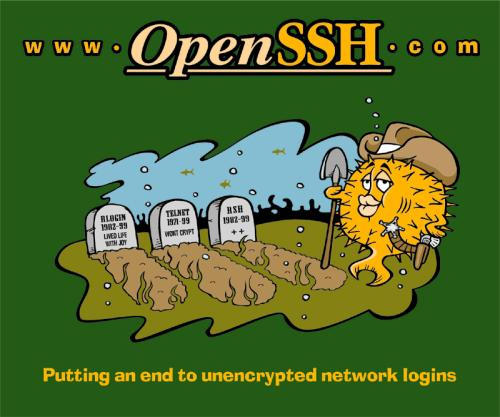
\includegraphics[width=12cm]{images/tshirt-9b.jpg}}  
%\end{center}

\hlkimage{16cm}{images/openssh-banner.png}

\begin{list1}
\item Hvad er Secure Shell SSH?  
\item Oprindeligt udviklet af Tatu Ylönen i Finland,\\
se \link{http://www.ssh.com}
\item SSH afl�ser en r�kke protokoller som er usikre:
  \begin{list2}
  \item Telnet til terminal adgang
  \item r* programmerne, rsh, rcp, rlogin, ...
  \item FTP med brugerid/password
  \end{list2}
\end{list1}


\slide{SSH - de nye kommandoer er}
\begin{list1}
\item kommandoerne er:
\begin{list2}
  \item ssh - Secure Shell
  \item scp - Secure Copy
  \item sftp - secure FTP 
  \end{list2}
\item Husk: SSH er b�de navnet p� protokollerne - version 1 og 2 samt
  programmet \verb+ssh+ til at logge ind p� andre systemer
\item SSH tillader ogs� port-forward, tunnel til usikre protokoller,
  eksempelvis X protokollen til UNIX grafiske vinduer
\item {\bfseries NB: Man b�r idag bruge SSH protokol version 2!}
\end{list1}


\slide{SSH n�gler}

I praksis benytter man n�gler fremfor kodeord
\begin{list1}
\item I kan lave jeres egne SSH n�gler med programmerne i Putty
\item Hvilken del skal jeg have for at kunne give jer adgang til en
  server?
\item Hvordan f�r jeg smartest denne n�gle?
\end{list1}

\slide{Installation af SSH n�gle}
\begin{list1}
\item Vi bruger login med password p� kurset, men for
  fuldst�ndighedens skyld beskrives her hvordan n�gle installeres:

\begin{list2}
\item f�rst skal der genereres et n�glepar {\bfseries id\_dsa og id\_dsa.pub}
\item Den offentlige del, filen id\_dsa.pub, kopieres til serveren
\item Der logges ind p� serveren 
\item Der udf�res f�lgende kommandoer:
\end{list2}
\end{list1}
\begin{alltt}
$ cd  \emph{skift til dit hjemmekatalog}
$ mkdir .ssh  \emph{lav et katalog til ssh-n�gler}
$ cat id\_dsa.pub >> .ssh/authorized\_keys  \emph{kopierer n�glen}
$ chmod -R go-rwx .ssh  \emph{skift rettigheder p� n�glen}
\end{alltt}


\slide{OpenSSH konfiguration}

\begin{list1}
\item S�dan anbefaler jeg at konfigurere OpenSSH SSHD
\item Det g�res i filen \verb+sshd_config+ typisk \verb+/etc/ssh/sshd_config+  
\end{list1}

\begin{alltt}
\small
Port 22780
Protocol 2

PermitRootLogin no
PubkeyAuthentication yes
AuthorizedKeysFile      .ssh/authorized_keys
# To disable tunneled clear text passwords, change to no here!
PasswordAuthentication no

#X11Forwarding no
#X11DisplayOffset 10
#X11UseLocalhost yes
\end{alltt}

Det er en smagssag om man vil tillade \emph{X11 forwarding}



\slide{VLAN Virtual LAN}

\hlkimage{10cm}{vlan-portbased.pdf}

\begin{list1}
\item Nogle switche tillader at man opdeler portene
\item Denne opdeling kaldes VLAN og portbaseret er det mest simple
\item Port 1-4 er et LAN
\item De resterende er et andet LAN
\item Data skal omkring en firewall eller en router for at krydse fra VLAN1 til VLAN2
\end{list1}

\slide{IEEE 802.1q}

\hlkimage{20cm}{vlan-8021q.pdf}

\begin{list1}
\item Nogle switche tillader at man opdeler portene, men tillige benytter 802.1q
\item Med 802.1q tillades VLAN tagging p� Ethernet niveau
\item Data skal omkring en firewall eller en router for at krydse fra VLAN1 til VLAN2
\item VLAN trunking giver mulighed for at dele VLANs ud p� flere switches
\item Der findes administrationsv�rkt�jer der letter dette arbejde: OpenNAC FreeNAC, Cisco VMPS
\end{list1}





\slide{IEEE 802.1x  Port Based Network Access Control}

\hlkimage{15cm}{osx-8021x.png}

\begin{list1}
\item Nogle switche tillader at man benytter 802.1x
\item Denne protokol sikrer at man valideres f�r der gives adgang til porten
\item N�r systemet skal have adgang til porten afleveres brugernavn og kodeord/certifikat
\item Denne protokol indg�r ogs� i WPA Enterprise
\end{list1}


\slide{802.1x og andre teknologier}

\begin{list1}
\item 802.1x i forhold til MAC filtrering giver v�sentlige fordele
\item MAC filtrering kan spoofes, hvor 802.1x kr�ver det rigtige kodeord
\item Typisk benyttes RADIUS og 802.1x integrerer s�ledes mod b�de LDAP og Active Directory
\end{list1}









%XXX \slide{input fra firewallskursus}




\slide{Hvad er en firewall}

\vskip 4 cm
\centerline{\hlkbig En firewall er noget som {\color{green}blokerer}
  traffik p� Internet}  

\vskip 1 cm
\pause

\centerline{\hlkbig En firewall er noget som {\color{red}tillader}
  traffik p� Internet}

\slide{Firewallrollen idag}

\begin{list1}
\item Idag skal en firewall v�re med til at:
\begin{list2}
\item Forhindre angribere i at komme ind
\item Forhindre angribere i at sende traffik ud
\item Forhindre virus og orme i at sprede sig i netv�rk
\item Indg� i en samlet l�sning med ISP, routere, firewalls, switchede
  strukturer, intrusion detectionsystemer samt andre dele af infrastrukturen
\end{list2}
\item Det kr�ver overblik!
\end{list1}


\slide{firewalls}

\begin{itemize}
\item Basalt set et netv�rksfilter - det yderste f�stningsv�rk
\item Indeholder typisk:
  \begin{list2}
   \item Grafisk brugergr�nseflade til konfiguration - er det en
   fordel?
\item TCP/IP filtermuligheder - pakkernes afsender, modtager, retning
  ind/ud, porte, protokol, ...
\item Kun IPv4 for de fleste kommercielle firewalls
\item B�de IPv4 og IPv6 for Open Source firewalls: IPF, OpenBSD PF,
  Linux firewalls, ...
\item Foruddefinerede regler/eksempler - er det godt hvis det er nemt
  at tilf�je/�bne en usikker protokol?
\item Typisk NAT funktionalitet indbygget
\item Typisk mulighed for nogle serverfunktioner: kan agere
  DHCP-server, DNS caching server og lignende
  \end{list2}
\item En router med Access Control Lists - ACL kaldes ofte
  netv�rksfilter, mens en dedikeret maskine kaldes firewall -
  funktionen er reelt den samme - der filtreres trafik
\end{itemize}


\slide{Packet filtering}

\begin{alltt}
\small
0                   1                   2                   3   
0 1 2 3 4 5 6 7 8 9 0 1 2 3 4 5 6 7 8 9 0 1 2 3 4 5 6 7 8 9 0 1 
+-+-+-+-+-+-+-+-+-+-+-+-+-+-+-+-+-+-+-+-+-+-+-+-+-+-+-+-+-+-+-+-+
|Version|  IHL  |Type of Service|          Total Length         |
+-+-+-+-+-+-+-+-+-+-+-+-+-+-+-+-+-+-+-+-+-+-+-+-+-+-+-+-+-+-+-+-+
|         Identification        |Flags|      Fragment Offset    |
+-+-+-+-+-+-+-+-+-+-+-+-+-+-+-+-+-+-+-+-+-+-+-+-+-+-+-+-+-+-+-+-+
|  Time to Live |    Protocol   |         Header Checksum       |
+-+-+-+-+-+-+-+-+-+-+-+-+-+-+-+-+-+-+-+-+-+-+-+-+-+-+-+-+-+-+-+-+
|                       Source Address                          |
+-+-+-+-+-+-+-+-+-+-+-+-+-+-+-+-+-+-+-+-+-+-+-+-+-+-+-+-+-+-+-+-+
|                    Destination Address                        |
+-+-+-+-+-+-+-+-+-+-+-+-+-+-+-+-+-+-+-+-+-+-+-+-+-+-+-+-+-+-+-+-+
|                    Options                    |    Padding    |
+-+-+-+-+-+-+-+-+-+-+-+-+-+-+-+-+-+-+-+-+-+-+-+-+-+-+-+-+-+-+-+-+  
\end{alltt}

\begin{list1}
\item Packet filtering er firewalls der filtrerer p� IP niveau
\item Idag inkluderer de fleste statefull inspection 
\end{list1}

\slide{Kommercielle firewalls}
\begin{list2}
\item Checkpoint Firewall-1 \link{http://www.checkpoint.com}
\item Nokia appliances - Nokia IPSO \link{http://www.nokia.com}
\item Cisco PIX \link{http://www.cisco.com}
\item Clavister firewalls \link{http://www.clavister.com}
\item Netscreen - nu ejet af Juniper
  \link{http://www.juniper.net}
\end{list2}

Ovenst�ende er dem som jeg oftest ser ude hos mine kunder

\slide{Open source baserede firewalls}
\begin{list2} 
\item Linux firewalls - fra begyndelsen til det nuv�rende netfilter
  til kerner version 2.4 og 2.6\\
\link{http://www.netfilter.org}
\item Firewall GUIs ovenp� Linux - mange! IPcop, Guarddog, Watchguard
nogle Linux firewalls er kommercielle produkter
\item IP Filter (IPF) \link{http://coombs.anu.edu.au/~avalon/}
\item OpenBSD PF - findes idag p� andre operativsystemer
\link{http://www.openbsd.org} 
\item FreeBSD IPFW og IPFW2 \link{http://www.freebsd.org}
\item Mac OS X benytter IPFW
\item FreeBSD inkluderer ogs� OpenBSD PF
\item NetBSD - bruger IPF og er ved at inkludere OpenBSD PF
\end{list2}

NB: kun eksempler og dem jeg selv har brugt


\slide{Hardware eller software}


\begin{list1}
\item Man h�rer indimellem begrebet \emph{hardware firewall}  
\item Det er dog et faktum at en firewall best�r af:
\begin{list2}
\item Netv�rkskort - som er hardware
\item Filtreringssoftware - som er \emph{software}!    
\end{list2}
\item Det giver ikke mening at kalde en Zyxel 10 en hardware firewall
  og en Soekris med OpenBSD for en software firewall!
\item Det er efter min mening et marketingtrick
\vskip 1 cm
\item Man kan til geng�ld godt argumentere for at en dedikeret
  firewall som en separat enhed kan give bedre sikkerhed
\end{list1}

\slide{TCP three way handshake}

\hlkimage{7cm}{images/tcp-three-way.pdf}

\begin{list2}
\item {\bfseries TCP SYN half-open} scans
\item Tidligere loggede systemer kun n�r der var etableret en fuld TCP
  forbindelse - dette kan/kunne udnyttes til \emph{stealth}-scans
\item Hvis en maskine modtager mange SYN pakker kan dette fylde
  tabellen over connections op - og derved afholde nye forbindelser
  fra at blive oprette - {\bfseries SYN-flooding}
\end{list2}

\slide{firewall regels�t eksempel}

\begin{alltt}
\tiny 
# hosts
router="217.157.20.129"
webserver="217.157.20.131"
# Networks
homenet="{ 192.168.1.0/24, 1.2.3.4/24 }"
wlan="10.0.42.0/24"
wireless=wi0

# things not used
spoofed="{ 127.0.0.0/8, 172.16.0.0/12, 10.0.0.0/16, 255.255.255.255/32 }"

block in all # default block anything
# loopback and other interface rules
pass out quick on lo0 all
pass in quick on lo0 all

# egress and ingress filtering - disallow spoofing, and drop spoofed
block in quick from $spoofed to any
block out quick from any to $spoofed

pass in on $wireless proto tcp from $wlan to any port = 22
pass in on $wireless proto tcp from $homenet to any port = 22
pass in on $wireless proto tcp from any to $webserver port = 80

pass out quick proto tcp  from $homenet to any flags S/S keep state
pass out quick proto udp  from $homenet to any         keep state
pass out quick proto icmp from $homenet to any         keep state
\end{alltt}
%$



\slide{netdesign - med firewalls - 100\% sikkerhed?}

\begin{center}
\colorbox{white}{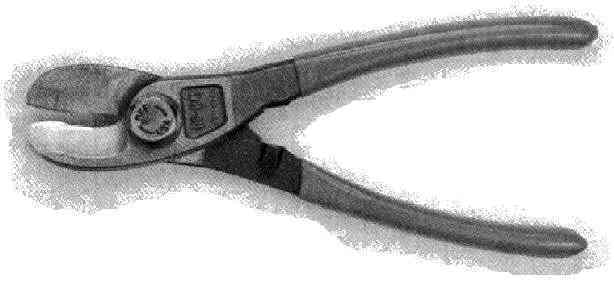
\includegraphics[width=12cm]{images/kut.jpg}}  
\end{center}

\begin{list1}
\item Hvor skal en firewall placeres for at g�re st�rst nytte?
\item Hvad er foruds�tningen for at en firewall virker?\\
At der er konfigureret et s�t fornuftige regler!
\item Hvor kommer reglerne fra? Sikkerhedspolitikken!
%\item Kan man lave en 100\% sikker firewall? Ja selvf�lgelig, se!
\end{list1}


\centerline{\small Kilde: Billedet er fra Marcus Ranum The ULTIMATELY
  Secure Firewall} 


\slide{Firewall er ikke alene}

\begin{list1}
\item Firewalls er ikke alene
\begin{list2}
\item anti-virus p� klienter og postsystemer
\item IDS systemer
\item Backupsystemer
\item Adgangskontrol
\item ... mange andre ting er mindst liges� vigtige
\end{list2}
\end{list1}

\centerline{\hlkbig Forsvaret er som altid - flere lag af sikkerhed! }


\slide{Firewall historik}


\hlkimage{6cm}{images/cheswick-cover2e.jpg}

\begin{list1}
\item Firewalls har v�ret kendt siden starten af 90'erne
\item Den f�rste bog \emph{Firewalls and Internet Security} udkom i
  1994 men der findes mange akademiske artikler om firewalls 
\item Bogen \emph{Firewalls and Internet Security} anbefales,  
William R. Cheswick, Steven M. Bellovin, Aviel D. Rubin,
Addison-Wesley, 2nd edition, 2003  
\end{list1}

\slide{An Evening with Berferd}


\begin{list1}
\item Artikel om en hacker der lokkes, vurderes, overv�ges
\item Et tidligt eksempel p� en honeypot
\item Idag anbefales The Honeynet Project hvis man vil vide mere
\\\link{http://www.honeynet.org}
\end{list1}




\slide{m0n0wall}

\hlkimage{20cm}{images/m0n0wall-1.pdf}


\slide{First or Last match firewall?}

\hlkimage{20cm}{images/first-last-match-1.pdf}


\slide{firewall koncepter}

\begin{list1}
\item R�kkef�lgen af regler betyder noget!
\begin{list2}
\item To typer af firewalls:
 First match - n�r en regel matcher, g�r det som angives block/pass
 Last match  - marker pakken hvis den matcher, til sidst afg�res block/pass
\end{list2}
\item {\bf Det er ekstremt vigtigt at vide hvilken type firewall
    man bruger!} 
\item OpenBSD PF er last match
\item FreeBSD IPFW er first match  
\item Linux iptables/netfilter er last match
\end{list1}

\slide{First or Last match firewall?}

\hlkimage{20cm}{images/first-last-match-1.pdf}
\begin{list2}
\item To typer af firewalls:
 First match - eksempelvis IPFW,
 Last match - eksempelvis PF
%\item {\bf Det er ekstremt vigtigt at vide hvilken type firewall
%    man bruger!} 
\end{list2}


\slide{First match - IPFW}

\begin{alltt}
\hlksmall
00100 16389  1551541 allow ip from any to any via lo0
00200     0        0 deny log ip from any to 127.0.0.0/8
00300     0        0 check-state
...
{\bfseries 
65435    36     5697 deny log ip from any to any}
65535   865    54964 allow ip from any to any
\end{alltt}

\vskip 2 cm

\centerline{Den sidste regel n�s aldrig!}

\slide{Last match - OpenBSD PF}

\begin{alltt}
\small
ext_if="ext0"
int_if="int0"

block in
pass out keep state

pass quick on \{ lo $int_if \}

# Tillad forbindelser ind p� port 80=http og port 53=domain
# p� IP-adressen for eksterne netkort ($ext_if) syntaksen
pass in on $ext_if proto tcp to ($ext_if) port http keep state
pass in on $ext_if proto \{ tcp, udp \} to ($ext_if) port domain keep state
\end{alltt}

\vskip 2 cm
\centerline{Pakkerne markeres med block eller pass indtil sidste
  regel}
\centerline{n�gleordet \emph{quick} afslutter match - god til store
  regels�t} 

\slide{Linux iptables/netfilter eksempel}

\begin{alltt}
\footnotesize
# Firewall configuration written by system-config-securitylevel
# Manual customization of this file is not recommended.
*filter
:INPUT ACCEPT [0:0]
:FORWARD ACCEPT [0:0]
:OUTPUT ACCEPT [0:0]
:RH-Firewall-1-INPUT - [0:0]
-A INPUT -j RH-Firewall-1-INPUT
-A FORWARD -j RH-Firewall-1-INPUT
-A RH-Firewall-1-INPUT -i lo -j ACCEPT
-A RH-Firewall-1-INPUT -p icmp --icmp-type any -j ACCEPT
-A RH-Firewall-1-INPUT -p 50 -j ACCEPT
-A RH-Firewall-1-INPUT -p 51 -j ACCEPT
-A RH-Firewall-1-INPUT -p udp --dport 5353 -d 224.0.0.251 -j ACCEPT
-A RH-Firewall-1-INPUT -p udp -m udp --dport 631 -j ACCEPT
-A RH-Firewall-1-INPUT -m state --state ESTABLISHED,RELATED -j ACCEPT
-A RH-Firewall-1-INPUT -m state --state NEW -m tcp -p tcp --dport 443 -j ACCEPT
-A RH-Firewall-1-INPUT -m state --state NEW -m tcp -p tcp --dport 22 -j ACCEPT
-A RH-Firewall-1-INPUT -j REJECT --reject-with icmp-host-prohibited
COMMIT
\end{alltt}

\centerline{NB: husk at aktivere IP forwarding}

\slide{Firewall GUI}

\hlkimage{24cm}{images/fwbuilder-screenshot1.png}

\begin{list1}
\item Der findes mange GUI programmer til Open Source firewalls
\end{list1}

Kilde: billede fra \link{http://www.fwbuilder.org}


\slide{m0n0wall}

\hlkimage{20cm}{images/m0n0wall-1.pdf}

Kilde: billede fra \link{http://m0n0.ch/wall/}

\slide{Firewalls og ICMP}


\begin{alltt}
ipfw add allow icmp from any to any icmptypes 3,4,11,12
\end{alltt}

\begin{list1}
\item Ovenst�ende er IPFW syntaks for at tillade de interessant ICMP beskeder igennem
\item Tillad ICMP types:
\begin{list2}
\item 3 Destination Unreachable
\item 4 Source Quench Message
\item 11 Time Exceeded
\item 12 Parameter Problem Message
\end{list2}
\end{list1}

\slide{Firewall konfiguration}

\begin{list1}
\item Den bedste firewall konfiguration starter med:
\begin{list2}
\item Papir og blyant
\item En fornuftig adressestruktur
\end{list2}
\item Brug dern�st en firewall med GUI f�rste gang!
\item Husk dern�st:
\begin{list2}
\item En firewall skal passes
\item En firewall skal opdateres
\item Systemerne bagved skal h�rdes!    
\end{list2}
\end{list1}

\slide{Bloker indefra og ud}

\begin{list1}
\item Der er porte og services som altid b�r blokeres
\item Det kan v�re kendte s�rbare services
\begin{list2}
\item Windows SMB filesharing - ikke til brug p� Internet!
\item UNIX NFS - ikke til brug p� Internet!
\end{list2}
\item Kendte problemer:
\begin{list2}
\item KaZaA og andre P2P programmer - hvis muligt!
\item Portmapper - port 111    
\end{list2}
\end{list1}

\slide{Firewall konfiguration}

\begin{list1}
\item Den bedste firewall konfiguration starter med:
\begin{list2}
\item Papir og blyant
\item En fornuftig adressestruktur
\end{list2}
\item Brug dern�st en firewall med GUI f�rste gang!
\item Husk dern�st:
\begin{list2}
\item En firewall skal passes
\item En firewall skal opdateres
\item Systemerne bagved skal h�rdes!    
\end{list2}
\end{list1}


\slide{En typisk firewall konfiguration}

\hlkimage{22cm}{images/firma-netvaerk.pdf}

\centerline{Opdeling i separate netv�rkssegmenter!}

\slide{personlige firewalls}

\begin{list1}
\item Personlige firewalls:  

\begin{list2}
\item Microsoft Windows XP
\item ZoneAlarm \link{http://www.zonelabs.com}  
\end{list2}
\item Personlige firewalls til Microsoft Windows inkluderer ofte
blokering af hvilket programmer der m� tilg� netv�rk
\end{list1}

\centerline{\color{titlecolor}Det anbefales at bruge en personlig firewall}

Note: Lad v�re med at stille sp�rgsm�l om logfilen i diverse fora!

{\bfseries Hvis du ikke forst�r loggen s� lad den ligge!}




\slide{Firewallv�rkt�jer}
% m�ske til reference afsnit?

\begin{list1}
\item Der benyttes p� kurset en del v�rkt�jer:
\begin{list2}
\item nmap - \link{http://www.insecure.org} portscanner
\item Nessus - \link{http://www.nessus.org} automatiseret testv�rkt�j
%\item libnet m.fl. - \link{http://www.packetfactory.net} - diverse projekter
%  relateret til pakker og IP netv�rk
%\item l0phtcrack - \link{http://www.atstake.com/research/lc/} - The Password
%  Auditing and Recovery Application
\item Ethereal - \link{http://www.ethereal.com} avanceret netv�rkssniffer
%\item F.I.R.E -  \link{http://biatchux.dmzs.com/} - en cd-rom der indeholder en 
%  bootable Linux del.
\item OpenBSD - \link{http://www.openbsd.org} operativsystem med fokus
  p� sikkerhed 
\item m0n0wall - \link{http://www.m0n0.ch} gratis firewall baseret p� FreeBSD

%\item \link{http://www.isecom.org/} - Open Source Security Testing
%  Methodology Manual - gennemgang af elementer der b�r indg� i en struktureret test 
\end{list2}
\end{list1}

\slide{Specielle features}

\begin{list2}
\item Network Address Translation - NAT
\item IPv6 funktionalitet

\item B�ndbredde h�ndtering
\item VLAN funktionalitet - mere udbredt i forbindelse med VoIP
\item Redundante firewalls - pfsync og CARP
% pfsync giver et indblik i hvordan den slags kan laves, hvor de
% kommercielle ``bare kan det''
\item IPsec og Andre VPN features
\end{list2}

\slide{Proxy servers}

\begin{list1}
\item Filtrering p� h�jere niveauer i OSI modellen er muligt
\item Idag findes proxy applikationer til de mest almindelige
  funktioner
\item Den typiske proxy er en caching webproxy der kan foretage HTTP
  request p� vegne af arbejdsstationer og gemme resultatet 
\item NB: nogle protokoller egner sig ikke til proxy servere
\item SSL forbindelser til \emph{secure websites} kan per design ikke proxies
\end{list1}

\slide{IPsec og Andre VPN features}

\begin{list1}
\item De fleste firewalls giver mulighed for at lave krypterede
  tunneler
\item Nyttigt til fjernkontorer der skal have usikker traffik henover
  usikre netv�rk som Internet 
\item Konceptet kaldes Virtual Private Network VPN
\item IPsec er de facto standarden for VPN og beskrevet i RFC'er 
\end{list1}


\slide{IPsec}

\begin{itemize}
\item Sikkerhed i netv�rket
\item RFC-2401 Security Architecture for the Internet Protocol
\item RFC-2402 IP Authentication Header (AH)
\item RFC-2406 IP Encapsulating Security Payload (ESP)
\item RFC-2409 The Internet Key Exchange (IKE) - dynamisk keying
\item B�de til IPv4 og IPv6
\item {\bfseries MANDATORY} i IPv6! - et krav hvis man implementerer
  fuld IPv6 support
\item god pr�sentation p� \link{http://www.hsc.fr/presentations/ike/}
\item Der findes IKEscan til at scanne efter IKE
  porte/implementationer\\
\link{http://www.nta-monitor.com/ike-scan/index.htm}
\end{itemize}

\slide{IPsec er ikke simpelt!}

\hlkimage{16cm}{images/ipsec-hsc.png}
\centerline{Kilde: \link{http://www.hsc.fr/presentations/ike/}}


\slide{RFC-2402 IP AH}

\begin{alltt}
\small
    0                   1                   2                   3
    0 1 2 3 4 5 6 7 8 9 0 1 2 3 4 5 6 7 8 9 0 1 2 3 4 5 6 7 8 9 0 1
   +-+-+-+-+-+-+-+-+-+-+-+-+-+-+-+-+-+-+-+-+-+-+-+-+-+-+-+-+-+-+-+-+
   | Next Header   |  Payload Len  |          RESERVED             |
   +-+-+-+-+-+-+-+-+-+-+-+-+-+-+-+-+-+-+-+-+-+-+-+-+-+-+-+-+-+-+-+-+
   |                 Security Parameters Index (SPI)               |
   +-+-+-+-+-+-+-+-+-+-+-+-+-+-+-+-+-+-+-+-+-+-+-+-+-+-+-+-+-+-+-+-+
   |                    Sequence Number Field                      |
   +-+-+-+-+-+-+-+-+-+-+-+-+-+-+-+-+-+-+-+-+-+-+-+-+-+-+-+-+-+-+-+-+
   |                                                               |
   +                Authentication Data (variable)                 |
   |                                                               |
   +-+-+-+-+-+-+-+-+-+-+-+-+-+-+-+-+-+-+-+-+-+-+-+-+-+-+-+-+-+-+-+-+
\end{alltt}

\slide{RFC-2402 IP AH}

Indpakning - pakkerne f�r og efter Authentication Header: 
\begin{alltt}
\small
                BEFORE APPLYING AH
            ----------------------------
      IPv4  |orig IP hdr  |     |      |
            |(any options)| TCP | Data |
            ----------------------------

                  AFTER APPLYING AH
            ---------------------------------
      IPv4  |orig IP hdr  |    |     |      |
            |(any options)| AH | TCP | Data |
            ---------------------------------
            |<------- authenticated ------->|
                 except for mutable fields
\end{alltt}

\slide{RFC-2406 IP ESP}

Pakkerne f�r og efter:
\begin{alltt}
\small 
               BEFORE APPLYING ESP
         ---------------------------------------
   IPv6  |             | ext hdrs |     |      |
         | orig IP hdr |if present| TCP | Data |
         ---------------------------------------



               AFTER APPLYING ESP
         ---------------------------------------------------------
   IPv6  | orig |hop-by-hop,dest*,|   |dest|   |    | ESP   | ESP|
         |IP hdr|routing,fragment.|ESP|opt*|TCP|Data|Trailer|Auth|
         ---------------------------------------------------------
                                   |<---- encrypted ---->|
                               |<---- authenticated ---->| 
\end{alltt}

\slide{ipsec konfigurationsfiler}

\begin{list1}
%\item Der er f�lgende dokumenter til IPsec p� websitet\\
% \link{www.security.net/courses/ipsec}:
\item Der er f�lgende filer tilg�ngelige\\
  \begin{list2}
  \item konfigurationsfiler i NetBSD/FreeBSD/Mac OS X format - med
    \verb+setkey+ kommandoen
  \item konfigurationsfil til OpenBSD server - med \verb+ipsecadm+
    kommandoen
%  \item IKE.pdf \emph{Dynamic Management of the IPsec Parameters:
%      The IKE Protocol}, fra Herve Schauer Consultants
%\item NetBSD IPsec dokumentation
%\item Cisco \emph{Introduction to IP security}
  \end{list2}
\end{list1}


\slide{IPsec setup}

%\hlkimage{}{images/}

\begin{list1}
  \item Client: Mac OS X/NetBSD/FreeBSD - samme syntaks\\
\verb+rc.ipsec.client+

\item Server: OpenBSD - bruger ipsecadm kommando\\
\verb+rc.ipsec.server+

\item �velse til l�seren: lav samme i Cisco IOS
\item Det vil ofte v�re relevant at se p� IOS og IPsec i laboratoriet
\item Dette setup n�r vi ikke at demonstrere
\end{list1}

\slide{rc.ipsec.client - client setup - adresser}

\begin{verbatim}
#!/bin/sh
# /etc/rc.ipsec.client - IPsec client configuration
# built from http://rt.fm/~jcs/ipsec_wep.phtml
# FreeBSD/NetBSD syntaks! - used on Mac OS X
# IPv4
SECSERVER=10.0.42.1
SECCLIENT=10.0.42.53
# IPv6
#SECSERVER=2001:618:433:101::1
#SECCLIENT=2001:618:433:101::153
ESPKEY=`cat ipsec.esp.key`
AHKEY=`cat ipsec.ah.key`
         
# Flush IPsec SAs in case we get called more than once
setkey -F
setkey -F -P
\end{verbatim}

\slide{rc.ipsec.client - client setup - SAs}

\begin{verbatim}
# Establish Security Associations
# 1000 is from the server to the client 
# 1001 is from the client to the server 
setkey -c <<EOF

add $SECSERVER $SECCLIENT esp 0x1000 \
-m tunnel -E blowfish-cbc 0x$ESPKEY  -A hmac-sha1 0x$AHKEY; 

add $SECCLIENT $SECSERVER esp 0x1001 \
-m tunnel -E blowfish-cbc 0x$ESPKEY -A hmac-sha1 0x$AHKEY; 

spdadd $SECCLIENT $SECSERVER any -P out \
ipsec esp/tunnel/$SECCLIENT-$SECSERVER/default;

spdadd $SECSERVER $SECCLIENT any -P in \
ipsec esp/tunnel/$SECSERVER-$SECCLIENT/default;
EOF
\end{verbatim}

\slide{rc.ipsec.server - server setup - adresser}

\begin{verbatim}
#!/bin/sh
#
# Henrik Lund Kramsh�j
# /etc/rc.ipsec - IPsec server configuration
# built from http://rt.fm/~jcs/ipsec_wep.phtml
# OpenBSD syntaks!
SECSERVER=10.0.42.1
SECCLIENT=10.0.42.53
#SECSERVER6=2001:618:433:101::1
#SECCLIENT6=2001:618:433:101::153

ESPKEY=`cat ipsec.esp.key`
AHKEY=`cat ipsec.ah.key`
         
# Flush IPsec SAs in case we get called more than once
ipsecadm flush
\end{verbatim}

        
\slide{rc.ipsec.server - server setup - SAs}

\begin{verbatim}
# Establish Security Associations
#
# 1000 is from the server to the client 
ipsecadm new esp -spi 1000 -src $SECSERVER -dst $SECCLIENT \
-forcetunnel -enc blf -key $ESPKEY \
-auth sha1 -authkey $AHKEY
         
# 1001 is from the client to the server 
ipsecadm new esp -spi 1001 -src $SECCLIENT -dst $SECSERVER \
-forcetunnel -enc blf -key $ESPKEY \
-auth sha1 -authkey $AHKEY
\end{verbatim}

        
\slide{rc.ipsec.server - server setup - flows}

\small
\begin{verbatim}
# Create flows
#
# Data going from the outside to the client
ipsecadm flow -out -src $SECSERVER -dst $SECCLIENT -proto esp \
-addr 0.0.0.0 0.0.0.0 $SECCLIENT 255.255.255.255 -dontacq
# IPv6
#ipsecadm flow -out -src $SECSERVER -dst $SECCLIENT -proto esp \
#-addr :: :: $SECCLIENT ffff:ffff:ffff:ffff:ffff:ffff:ffff:ffff -dontacq
     
# Data going from the client to the outside
ipsecadm flow -in -src $SECSERVER -dst $SECCLIENT -proto esp \
-addr $SECCLIENT 255.255.255.255 0.0.0.0 0.0.0.0 -dontacq                  
# IPv6
#ipsecadm flow -in -src $SECSERVER -dst $SECCLIENT -proto esp \
#-addr :: :: $SECCLIENT ffff:ffff:ffff:ffff:ffff:ffff:ffff:ffff -dontacq
\end{verbatim}



%%% Local Variables: 
%%% mode: latex
%%% TeX-master: t
%%% End: 


\slide{OpenVPN / OpenSSL VPN}

\begin{quote}
OpenVPN is a full-featured SSL VPN solution which can accomodate a
wide range of configurations, including remote access, site-to-site
VPNs, WiFi security, and enterprise-scale remote access solutions with
load balancing, failover, and fine-grained access-controls (articles)
(examples) (security overview) (non-english languages).   
\end{quote}

\begin{list1}
\item Et andet popul�rt VPN produkt er OpenVPN
\item Bem�rk dog at hvis der benyttes TCP i TCP risikerer man at st�de ind i 
et problem som kaldes \emph{TCP in TCP meltdown} 
\item Kilde: \link{http://openvpn.net/}  
\end{list1}



\exercise{ex:unix-basic-firewall}










\slide{Portscan, TCP, UDP og ICMP}

Forskellen mellem TCP og UDP i forbindelse med portscan, og effekten af en firewall der dropper pakker

\slide{Basal Portscanning}

\begin{list1}
  \item Hvad er portscanning
\item afpr�vning af alle porte fra 0/1 og op til 65535
\item m�let er at identificere �bne porte - s�rbare services
\item typisk TCP og UDP scanning
\item TCP scanning er ofte mere p�lidelig end UDP scanning
\end{list1}

{\hlkbig TCP handshake er nemmere at identificere

UDP applikationer svarer forskelligt - hvis overhovedet}

\slide{TCP three way handshake}

\hlkimage{7cm}{images/tcp-three-way.pdf}

\begin{list2}
\item {\bfseries TCP SYN half-open} scans
\item Tidligere loggede systemer kun n�r der var etableret en fuld TCP
  forbindelse - dette kan/kunne udnyttes til \emph{stealth}-scans
\item Hvis en maskine modtager mange SYN pakker kan dette fylde
  tabellen over connections op - og derved afholde nye forbindelser
  fra at blive oprette - {\bfseries SYN-flooding}
\end{list2}


\slide{Ping og port sweep}

\begin{list1}
\item scanninger p� tv�rs af netv�rk kaldes for sweeps 
\item Scan et netv�rk efter aktive systemer med PING
\item Scan et netv�rk efter systemer med en bestemt port �ben
\item Er som regel nemt at opdage:
  \begin{list2}
    \item konfigurer en maskine med to IP-adresser som ikke er i brug
\item hvis der kommer trafik til den ene eller anden er det portscan
\item hvis der kommer trafik til begge IP-adresser er der nok
  foretaget et sweep - bedre hvis de to adresser ligger et stykke fra hinanden
  \end{list2}

\end{list1}

\slide{nmap port sweep efter port 80/TCP}

\begin{list1}
  \item Port 80 TCP er webservere
\end{list1}

\begin{alltt}
\small # {\bfseries nmap  -p 80 217.157.20.130/28}

Starting nmap V. 3.00 ( www.insecure.org/nmap/ )
Interesting ports on router.kramse.dk (217.157.20.129):
Port       State       Service
80/tcp     filtered    http                    

Interesting ports on www.kramse.dk (217.157.20.131):
Port       State       Service
80/tcp     open        http                    

Interesting ports on  (217.157.20.139):
Port       State       Service
80/tcp     open        http                    

\end{alltt}

\slide{nmap port sweep efter port 161/UDP}

\begin{list1}
  \item Port 161 UDP er SNMP
\end{list1}

\begin{alltt}  
\small # {\bfseries nmap -sU -p 161 217.157.20.130/28}

Starting nmap V. 3.00 ( www.insecure.org/nmap/ )
Interesting ports on router.kramse.dk (217.157.20.129):
Port       State       Service
161/udp    open        snmp                    

The 1 scanned port on mail.kramse.dk (217.157.20.130) is: closed

Interesting ports on www.kramse.dk (217.157.20.131):
Port       State       Service
161/udp    open        snmp                    

The 1 scanned port on  (217.157.20.132) is: closed
\end{alltt}

\slide{OS detection}
\begin{alltt}
\footnotesize
# nmap -O ip.adresse.slet.tet \emph{scan af en gateway}
Starting nmap 3.48 ( http://www.insecure.org/nmap/ ) at 2003-12-03 11:31 CET
Interesting ports on gw-int.security6.net (ip.adresse.slet.tet):
(The 1653 ports scanned but not shown below are in state: closed)
PORT     STATE SERVICE
22/tcp   open  ssh
80/tcp   open  http
1080/tcp open  socks
5000/tcp open  UPnP
Device type: general purpose
Running: FreeBSD 4.X
OS details: FreeBSD 4.8-STABLE
Uptime 21.178 days (since Wed Nov 12 07:14:49 2003)
Nmap run completed -- 1 IP address (1 host up) scanned in 7.540 seconds
\end{alltt}

\begin{list2}
  \item lavniveau m�de at identificere operativsystemer p�
\item send pakker med \emph{anderledes} indhold
\item Reference: \emph{ICMP Usage In Scanning} Version 3.0,
  Ofir Arkin\\ \link{http://www.sys-security.com/html/projects/icmp.html}
\end{list2}

\slide{Top 75 Security Tools}

\begin{list1}
%  \item I er meget ivrige efter at afpr�ve en masse
\item listen over 75 top security
  tools - nogle v�rkt�jer springes over, nogle har vi brugt
\item Den er samlet af Fyodor og findes p�:\\
\link{http://www.insecure.org/tools.html}
\end{list1}


\slide{Hvad skal der ske?}

\begin{list1}
\item T�nk som en hacker
\item Rekognoscering
\begin{list2}
\item ping sweep, port scan
\item OS detection - TCP/IP eller banner grab
\item Servicescan - rpcinfo, netbios, ...
\item telnet/netcat interaktion med services
\end{list2}
\item Udnyttelse/afpr�vning: Nessus, nikto, exploit programs
\item Oprydning vises ikke p� kurset, men I b�r i praksis:
\begin{list2}
\item Lav en rapport
\item Gennemg� rapporten, registrer �ndringer
\item Opdater programmer, konfigurationer, arkitektur, osv. 
\end{list2}
\item I skal jo ogs� VISE andre at I g�r noget ved sikkerheden.
\end{list1}


\exercise{ex:nmap-sweep}
\exercise{ex:nmap-portscan}
\exercise{ex:nmap-service}
\exercise{ex:nmap-os}



\slide{Firewalls og IPv6}

\begin{list1}
\item L�g m�rke til forskellen mellem ARP og ICMPv6  
\item Hvis det er muligt lav een regel der tillader adgang til services uanset protokol
\item NB: husk at aktivere IP forwarding n�r I skal lave en firewall
\end{list1}


\slide{OpenBSD PF}
\begin{alltt}
\footnotesize
# Macros: define common values, so they can be referenced and changed easily.
int_if=vr0
ext_if=vr2
tunnel_if=gif0
table <homenet6> { 2001:16d8:ffd2:cf0f::/64 }
set skip on lo0
scrub in all
# Filtering: the implicit first two rules are
block in all
block out all
# allow ICMPv6 for NDP
pass in inet6 proto ipv6-icmp all icmp6-type neighbradv keep state
# server with configured IP address and router advertisement daemon running
pass out inet6 proto ipv6-icmp all icmp6-type routersol keep state
# client which uses autoconfiguration would use this instead
#pass in inet6 proto ipv6-icmp all icmp6-type routeradv keep state
#pass out inet6 proto ipv6-icmp all icmp6-type neighbrsol keep state
table <sixxspop> { 82.96.56.14 2001:16d8:ff00:155::1 }
pass in on $ext_if proto icmp from <sixxspop6> to ($ext_if)
pass in on $tunnel_if proto icmp6 from <sixxspop6> to any
pass in on $int_if all
pass out on $int_if all keep state
...  probably not working AS IS
\end{alltt}


\slide{Redundante firewalls}

\hlkimage{8cm}{images/pfsync-carp-1.jpg}

\begin{list2}
\item OpenBSD Common Address Redundancy Protocol CARP - b�de IPv4 og IPv6\\
overtagelse af adresse b�de IPv4 og IPv6
\item pfsync - sender opdateringer om firewall states mellem de to systemer  
\item Kilde:
\link{http://www.countersiege.com/doc/pfsync-carp/}
\end{list2}

\slide{Redundante forbindelser hardware}

\begin{alltt}
root@azumi:# cat hostname.fxp0
up
root@azumi:# cat hostname.fxp1 
up
root@azumi:# cat /etc/hostname.trunk0
trunkproto failover trunkport fxp0 trunkport fxp1
dhcp
\end{alltt}

\begin{list1}
\item OpenBSD trunk interface
\item Linux bonding, 
\item Etherchannel Cisco
\item Idag anbefales IEEE 802.3ad LACP som er en �ben standard
\item \link{http://en.wikipedia.org/wiki/EtherChannel}
\end{list1}

\slide{LACP Link Aggregation Control Protocol}

\hlkimage{7cm}{lacp-1.pdf}

\begin{list1}
\item IEEE 802.3ad standardiseret bundling/failover
\item M�let er at give:
\begin{list2}
\item mere b�ndbredde end en enkelt port
\item failover - hvis et link falder ud
\end{list2}
\item En server med to netinterfaces kan med fordel forbindes til to porte
\item Er ikke generelt underst�ttet i alle operativsystemer, men det kommer
\item \link{http://en.wikipedia.org/wiki/Link_Aggregation_Control_Protocol}
\end{list1}


\slide{Redundante forbindelser IP-niveau}

\hlkimage{12cm}{router-redundancy-1.pdf}

\begin{list1}
\item HSRP Hot Standby Router Protocol, Cisco protokol, RFC-2281
\item VRRP Virtual Router Redundancy Protocol, IETF RFC-3768, �ben standard - ikke fri
\item CARP Common Address Redundancy Protocol, findes p� OpenBSD og FreeBSD
\item \link{http://en.wikipedia.org/wiki/Common_Address_Redundancy_Protocol}
\end{list1}








\slide{Mobile IP}

\begin{list1}
\item Mobility er ved at blive et krav, idet enheder idag er mobile
\item Specielt �nsker vi at h�ndholdte computere og laptops kan modtage data
\item Tidligere skiftede man blot adresse undervejs
\item Idag �nsker man at enheden kan kontaktes nemmere, selv udenfor \emph{huset}
\item RFC-3344 IP Mobility Support for IPv4
\item RFC-4721 Mobile IPv4 Challenge/Response Extensions (Revised)
\item RFC-3775
\item \link{http://en.wikipedia.org/wiki/Mobile_IP}
\item Bem�rk at Mobile IP ikke altid er n�dvendig eller benyttes, mange protokoller som eksempelvis POP3/IMAP virker fint ved at enheden kalder tilbage til serveren
\end{list1}

\slide{Mobile IP begreber}

\begin{list1}
\item Definitioner - fra RFC-3344:
\begin{list2}
\item Mobile Node A host or router that changes its point of attachment from one
         network or subnetwork to another. 
\item Home Agent A router on a mobile node's home network which tunnels
         datagrams for delivery to the mobile node when it is away from
         home, and maintains current location information for the mobile
         node.
\item Foreign Agent A router on a mobile node's visited network which provides
         routing services to the mobile node while registered.  The
         foreign agent detunnels and delivers datagrams to the mobile
         node that were tunneled by the mobile node's home agent.  For
         datagrams sent by a mobile node, the foreign agent may serve as
         a default router for registered mobile nodes.
\end{list2}
\item Selve funktionen:\\
   A mobile node is given a long-term IP address on a home network.
   This home address is administered in the same way as a "permanent" IP
   address is provided to a stationary host.  When away from its home
   network, a "care-of address" is associated with the mobile node and
   reflects the mobile node's current point of attachment. 
\end{list1}

\slide{Oversigt Mobile IP}

\hlkimage{23cm}{mobile-ip-1.pdf}

Se ogs� Mobile IPv6 A short introduction \link{http://www.hznet.de/ipv6/mipv6-intro.pdf}


\slide{VoIP Voice over IP}

\begin{list1}
\item Tidligere havde vi adskilte netv�rk, nu samles de 
\item Idag er det meget normalt at b�de firmaer og private bruger IP-telefoni
\item Fordele er prim�rt billigere og mere fleksibelt
\item Eksempler p� IP telefoni:
\begin{list2}
\item Skype benytter IP, men egenudviklet protokol
\item Cisco IP-telefoner benyttes ofte i firmaer
\item Cybercity telefoni k�rer over IP, med analog adapter
\end{list2}
\item Det anbefales at se p� Asterisk telefoniserver, hvis man har mod p� det :-)
\item \link{http://www.asterisk.org/}
\end{list1}

\slide{VoIP bekymringer}

\begin{list1}
\item Der er generelt problemer med:
\begin{list2}
\item Stabilitet - quality of service, netv�rket skal v�re bygget til det
\item Sikkerhed - hvem lytter med, hvem kan afbryde forbindelsen\\
Se evt. \link{http://www.voipsa.org/}
\item Spam over VoIP, connect, send WAV fil med spam kaldes SPIT
\item Kompatabilitet - hvilke protokoller, codecs, standarder, ...
\end{list2}
\item Der er flere store spillere
\end{list1}

\slide{VoIP protokoller}

\begin{list1}
\item SIP Session Initiation Protocol, IETF standard signaleringsprotokol
\item H.323 ITU-T standard signaleringsprotokol
\item IAX Inter-Asterisk Exchange Protocol, Asterisk protokol
\item SSCP Cisco protokol
\item ZRTP Phil Zimmermann, zfone - sikker kommunikation\\ 
\link{http://zfoneproject.com/}
\end{list1}

\slide{Dag 5 Diverse}

\hlkimage{20cm}{openbgpd-network-1.pdf}




\slide{Opsamling}

\begin{list1}
\item Dagen idag er prim�rt beregnet til opsamling
\item Detaljer som ikke har v�ret gennemg�et undervejs, fordi jeg mente det var bedre at sk�rme imod i den f�rste gennemgang

\end{list1}

\slide{Internet-relaterede organisationer}

\hlkimage{20cm}{IAB_structure.pdf}

\centerline{Oftest er man interesseret i \link{http://www.ietf.org/}}

\slide{Proxy-arp}

\begin{list1}
\item Routere underst�tter ofte Proxy ARP
\item Med Proxy ARP svarer de for en adresse bagved routeren
\item Derved kan man f� trafik nemt igennem fra internet til adresser
\item Det er smart i visse situationer hvor en subnetting vil spilde for mange adresser
\item Hvis man kun har f� adresser er subnetting m�ske heller ikke muligt
\item \link{http://en.wikipedia.org/wiki/Proxy_ARP}
\end{list1}

\slide{Reverse ARP}

\begin{list1}
\item Tidligere brugte man en protokol kaldet Reverse ARP til at uddele IP-adresser
\item Med Reverse ARP sender en enhed et request og f�r et Reverse ARP svar tilbage
\item \emph{Jeg har denne MAC adresse, hvad er min IP?}
\item \emph{Hvis du er denne MAC adresse er din IP 10.2.3.1}
\item Det benyttes meget sj�ldent idag, men var tidligere brugt til netboot af arbejdsstationer m.v.
\end{list1}

\slide{ICMP redirect}

\begin{list1}
\item Routere underst�tter ofte ICMP Redirect
\item Med ICMP Redirect kan man til en afsender fort�lle en anden vej til destination
\item Den angivne vej kan v�re smartere eller mere effektiv
\item Det er desv�rre uheldigt, idet der ingen sikkerhed er
\item Idag b�r man ikke lytte til ICMP redirects, ej heller generere dem
\item Det svarer til ARP spoofing, idet trafik omdirigeres
\end{list1}


\slide{Hvordan virker ARP spoofing?}

\begin{center}
\colorbox{white}{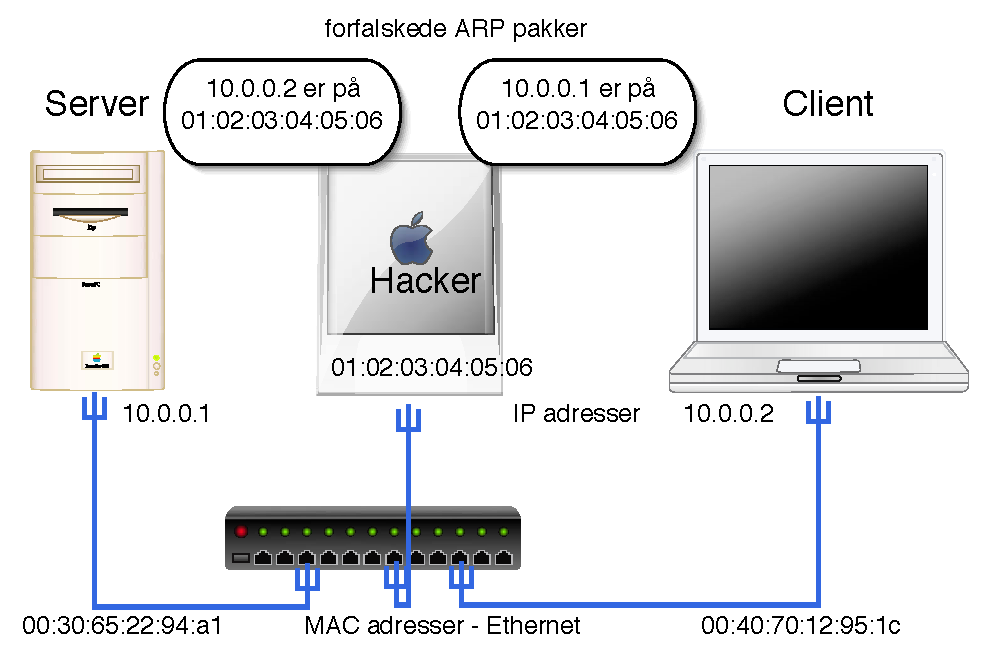
\includegraphics[width=15cm]{images/arp-spoof.pdf}}  
\end{center}

\begin{list1}
\item Hackeren sender forfalskede ARP pakker til de to parter
\item De sender derefter pakkerne ud p� Ethernet med hackerens MAC
  adresse som modtager - han f�r alle pakkerne
\end{list1}

\slide{Forsvar mod ARP spoofing}

\begin{list1}
\item Hvad kan man g�re? 
\item l�se MAC adresser til porte p� switche
\item l�se MAC adresser til bestemte IP adresser
\item Efterf�lgende administration!
\vskip 1 cm
\item {\bfseries arpwatch er et godt bud} - overv�ger ARP
\item bruge protokoller som ikke er s�rbare overfor opsamling
\end{list1}


\slide{IGMP Internet Group Management Protocol}

\begin{list1}
\item Der er defineret Multicast protokoller p� internet
\item Med multicast kan man sende data til en n�rmere angivet gruppe
\item Multicast er tilt�nkt ting som radio og video broadcast
\item IPv6 benytter en del multicast adresser, all-nodes, all-routes, ...
\item Hvem der modtager data styres s� ved hj�lp af IGMP
\item IGMP bruges s�ledes til at styre hvem der p� et givet tidspunkt er med i IP multicast grupper
\item RFC-3376 Internet Group Management Protocol, Version 3
\item \link{http://en.wikipedia.org/wiki/Internet_Group_Management_Protocol}
\end{list1}


\slide{TCP sequence number prediction}

\begin{list1}
  \item tidligere baserede man ofte login og adgange p� de IP adresser
  som folk kom fra
\item det er ikke p�lideligt at tro p� address based authentication
\item TCP sequence number kan m�ske g�ttes
\item Mest kendt er nok Shimomura der blev hacket p� den m�de, m�ske
  af Kevin D Mitnick eller en kompagnon
\item I praksis vil det v�re sv�rt at udf�re p� moderne operativsystemer
\item Se evt. \link{http://www.takedown.com/}
\item (filmen er ikke s� god ;-) ) 
\end{list1}


\slide{Hardware IPv4 checksum offloading}

\begin{list1}
\item IPv4 checksum skal beregnes hvergang man modtager en pakke
\item IPv4 checksum skal beregnes hvergang man sender en pakke
\vskip 1cm
\item Lad en ASIC g�re arbejdet!
\item De fleste servernetkort tilbyder at foretage denne beregning p� IPv4
\item IPv6 benytter ikke header checksum, det er un�dvendigt
\end{list1}
\vskip 1cm

\centerline{\hlkbig NB: kan resultere i at tcpdump siger checksum er forkert!}


\slide{At v�re p� internet}

\begin{list1}
\item RFC-2142 Mailbox Names for Common Services, Roles and Functions
\item Du B�R konfigurere dit dom�ne til at modtage post for f�lgende adresser:
\begin{list2}
\item postmaster@dom�ne.dk
\item abuse@dom�ne.dk
\item webmaster@dom�ne.dk, evt. www@dom�ne.dk
\end{list2}
\item Du g�r det nemmere at rapportere problemer med dit netv�rk og services
\end{list1}

\slide{E-mail best current practice}

\begin{alltt}
MAILBOX       AREA                USAGE
-----------   ----------------    ---------------------------
ABUSE         Customer Relations  Inappropriate public behaviour
NOC           Network Operations  Network infrastructure
SECURITY      Network Security    Security bulletins or queries  
...
MAILBOX       SERVICE             SPECIFICATIONS
-----------   ----------------    ---------------------------
POSTMASTER    SMTP                [RFC821], [RFC822]
HOSTMASTER    DNS                 [RFC1033-RFC1035]
USENET        NNTP                [RFC977]
NEWS          NNTP                Synonym for USENET
WEBMASTER     HTTP                [RFC 2068]
WWW           HTTP                Synonym for WEBMASTER
UUCP          UUCP                [RFC976]
FTP           FTP                 [RFC959]
\end{alltt}

Kilde: 
RFC-2142 Mailbox Names for Common Services, Roles and Functions. D.
Crocker. May 1997

\slide{Brug krypterede forbindelser}

\hlkimage{18cm}{images/dsniff-comments.pdf}

\begin{list1}
\item Is�r p� utrov�rdige netv�rk kan det give problemer at benytte
  s�rbare protokoller   
\end{list1}

\slide{Mission 1: Kommunikere sikkert}

\begin{list1}
\item Du m� ikke bruge ukrypterede forbindelser til at administrere
  UNIX
\item Du m� ikke sende kodeord i ukrypterede e-mail beskeder  
\end{list1}

\centerline{\hlkbig Telnet daemonen - telnetd m� og skal d�!}

\pause
\centerline{\hlkbig FTP daemonen - ftpd m� og skal d�!}

\pause
\centerline{\hlkbig POP3 daemonen port 110 m� og skal d�!}

\pause
\centerline{\hlkbig IMAPD daemonen port 143 m� og skal d�!}

\pause
\vskip 1cm 
\centerline{\hlkbig\bf v�k med alle de ukrypterede forbindelser!}


\slide{Infrastrukturer i praksis}

\begin{list1}
\item Vi vil nu gennemg� netv�rksdesign med udgangspunkt i vores setup
\item Vores setup indeholder:
\begin{list2}
\item Routere
\item Firewall
\item Wireless
\item DMZ
\item DHCPD, BIND, BGPD, OSPFD, ...
\end{list2}
\item Den kunne udvides med flere andre teknologier vi har til r�dighed:
\begin{list2}
\item VLAN inkl VLAN trunking/distribution
\item WPA Enterprise
\end{list2}
\item Hvad taler for og imod - de n�ste slides gennemg�r nogle standardsetups
\item En slags Patterns for networking
\end{list1}





\slide{Netv�rksdesign og sikkerhed}

\begin{list1}
\item Hvad kan man g�re for at f� bedre netv�rkssikkerhed?
\begin{list2}
\item Bruge switche - der skal ARP spoofes og bedre performance
\item Opdele med firewall til flere DMZ zoner for at holde
      udsatte servere adskilt fra hinanden, det interne netv�rk og
      Internet
\item Overv�ge, l�se logs og reagere p� h�ndelser 
\end{list2}
\item Husk du skal ogs� kunne opdatere dine servere
\end{list1}

\slide{basalt netv�rk}

\hlkimage{16cm}{images/demo-netvaerk.pdf}

\begin{list1}
\item Du b�r opdele dit netv�rk i segmenter efter traffik
\item Du b�r altid holde interne og eksterne systemer adskilt!
\item Du b�r isolere farlige services i jails og chroots
\end{list1}



\slide{Intrusion Detection Systems - IDS}

\begin{list1}
  \item angrebsv�rkt�jerne efterlader spor

\item hostbased IDS - k�rer lokalt p� et system og fors�ger at
  detektere om der er en angriber inde
\item network based IDS - NIDS - bruger netv�rket
\item Automatiserer netv�rksoverv�gning:
  \begin{list2}
  \item bestemte pakker kan opfattes som en signatur
\item analyse af netv�rkstrafik - F�R angreb
\item analyse af netv�rk under angreb - sender en alarm
  \end{list2}
\item \link{http://www.snort.org} - det kan anbefales at se p� Snort
\end{list1}

\slide{snort}

\hlkimage{5cm}{images/snort_tm.png}

\begin{list1}
\item Snort er Open Source og derfor godt til undervisning
\item man kan se det som et antivirus system til netv�rket
\item fors�ger at detektere \emph{angreb}, \emph{skadelig} og
  \emph{forkert} traffik
\item pakker der minder om eksempelvis:
  \begin{list2}
    \item nmap portscan
\item nmap OS detection - med underlige pakker
\item fragmenter der overlapper
\item shellcode der sendes til systemer som BIND
  \end{list2}
\end{list1}

\slide{Snort regler}

\begin{alltt}\small
alert icmp $HOME_NET any -> $EXTERNAL_NET any (msg:"ICMP Address Mask
Reply"; icode:0; itype:18; classtype:misc-activity; sid:386; rev:5;)
alert icmp $EXTERNAL_NET any -> $HOME_NET any (msg:"ICMP Address Mask 
Reply undefined code"; icode:>0; itype:18; classtype:misc-activity; 
sid:387; rev:7;)
alert icmp $EXTERNAL_NET any -> $HOME_NET any (msg:"ICMP Address Mask 
Request"; icode:0; itype:17; classtype:misc-activity; sid:388; rev:5;)
alert icmp $EXTERNAL_NET any -> $HOME_NET any (msg:"ICMP Address Mask 
Request undefined code"; icode:>0; itype:17; classtype:misc-activity; 
sid:389; rev:7;)
alert icmp $EXTERNAL_NET any -> $HOME_NET any (msg:"ICMP Alternate 
Host Address"; icode:0; itype:6; classtype:misc-activity; sid:390; rev:5;)
\end{alltt}

\begin{list2}
\item sid - snort rules id - identificerer en signatur  
\item reference - hvor kommer reglen fra
\item icode - ICMP code
\item itype - ICMP type
\item ... se mere i snort manualen
\end{list2}

\slide{Ulemper ved IDS}

\hlkimage{5cm}{images/snort_tm.png}

\begin{list1}
\item snort er baseret p� signaturer
\item mange falske alarmer - tuning og vedligehold
\item hvordan sikrer man sig at man har opdaterede signaturer for
  angreb som g�r verden rundt p� et d�gn 
\end{list1}

\slide{ Planl�gning af IDS milj�er}

\begin{list1}
\item F�r installationen
\begin{list2}
\item Hvad er form�let - reaktion eller "statistik"
\item Hvor skal der m�les - hele netv�rket eller specifikke dele
\item Hvad skal m�les og hvilke operativsystemer og servere/services
\end{list2}
\item Implementationen
\begin{list2}
\item Er infrastrukturen iorden som den er
\item Er der gode m�lepunkter - monitorporte
\item Et m�lepunkt eller flere
\item Hvormeget trafik skal m�les
\end{list2}
\item Selve idrifts�ttelsen
\begin{list2}
\item �ndringer af infrastrukturen
\item Installation af udstyret
\item Test af udstyret udenfor drift
\item Installation i driftsmilj�et
\item Test af udstyret i driftsmilj�et
\end{list2}
\end{list1}

\slide{ Ops�tning og konfiguration af IDS milj�er}

\begin{list1}
\item V�lg en simpel installation til at starte med!
\item Undg� for alt i verden for meget information
\begin{list2}
\item Start med en enkelt sensor
\item Byg en server med database og "brugerv�rkt�jer"
\item Start med at overv�ge dele af nettet
\item Brug et specifikt regels�t i starten - eksempelvis kun Windows eller kun UNIX
\item Lav nogle simple rapporter til at starte med
\end{list2}
\item G�r netv�rket mere sikkert f�r du lytter p� hele netv�rket
\item Brug tcpdump/Ethereal til at se p� trafik, l�r IP pakker at
  kende 
\item Brug Snort til at evaluere
\begin{list2}
\item husk at man kan starte med Snort og senere skifte til andre
produkter
\item Erfaring t�ller, Snort tillader at man ser de fine detaljer - motoren
\end{list2}
\end{list1}

\slide{ Vedligehold og overv�gning af IDS milj�er}

\begin{list1}
\item Uden vedligehold er IDS v�rdil�st - lad hellere v�re!
\begin{list2}
\item Vedligehold af software p� operativsystemet
\item Vedligehold af IDS softwaren
\item Vedligehold af regels�t
\end{list2}
\item Overv�gning - k�rer IDS systemet, databaser og sensorer
\item Statistik og brug af IDS systemet
\begin{list2}
\item Vedligehold af rapporter - hvad er vi interesseret i
\item Automatisk rapportgenerering - daglig rapport, rapport pr m�ned
\item Specielle h�ndelser - hvad skete der onsdag mellem 11-12
\end{list2}
\item Et IDS kan ogs� blot v�re en ARPwatch
\item ARPwatch advarer hvis nogen tager adressen fra default gateway
\end{list1}


\slide{Honeypots}

\begin{list1}
\item Man kan udover IDS installere en honeypot
\item En honeypot best�r typisk af:
  \begin{list2}
    \item Et eller flere s�rbare systemer
\item Et eller flere systemer der logger traffik til og fra honeypot
  systemerne 
  \end{list2}
\item Meningen med en honeypot er at den bliver angrebet og brudt ind
  i 
\end{list1}

%\slide{Prelude}

%M�ske Prelude i kombination med Nagios, Cricket, MRTG, RRDTool, Smokeping, ARPwatch


%\slide{Oversigt over forsvar mod s�rbarheder}

\begin{list1}
\item Hvad muligheder har man
  \begin{list2}
  \item �ndre milj�
  \item forbedre systemerne
  \item undg� standardindstillinger
  \item v�r opdateret p� sikkerhedsomr�det
  \item have retningslinier - ens sikkerhedsniveau
  \item drop kompatibilitet med usikre systemer
  \item en god infrastruktur
  \item brug kryptografi
  \item brug standardbiblioteker
  \item test af systemer
  \end{list2}
\end{list1}

\slide{�ndre milj�}

\begin{list1}
\item �ndre arkitektur sw/hw/netv�rkstopologi
  \begin{list2}
  \item blokere porte s�ledes at en webserver IKKE kan connecte tilbage til hackeren!
  \item blokere de services der IKKE skal tilg�s udefra
  \item skifte programmeringssprog
  \end{list2}
\item Husk altid at hackeren ogs� kan g� ind ad hoved�ren
\item eksempelvis SAP Internet gateway, hvor man kunne l�gge det
  bagvedliggende system ned med loginrequests
\end{list1}
\slide{Forbedre systemerne}

\begin{list1}
\item Operativsystemet
  \begin{list2}
  \item non-executable stack
  \item non-executable heap
  \end{list2}
\item Applikationsservere
  \begin{list2}
  \item filtrering af "d�rlige" requests e-Eye sikret IIS
  \item mere "sikker" default ops�tning
  \end{list2}
\item Jeg tror vi vil se flere implementere den slags l�sninger
\item Eksempelvis:
\begin{list2}
\item Microsoft IIS web server version 6 er mere sikker i default ops�tningen  
\item Apache HTTPD web server version 2 er mere modul�r og nemmere at bygge sikkert  
\end{list2}
\end{list1}

\slide{Undg� standard indstillinger}

\begin{list1}
\item Giv jer selv mere tid til at patche og opdatere
\item Tiden der g�r fra en s�rbarhed annonceres p� bugtraq til den bliver
       udnyttet er meget kort idag!
\item Ved at undg� standard indstillinger kan der
       m�ske opn�s en lidt l�ngere frist - inden ormene kommer
\item NB: ingen garanti
\end{list1}



\slide{Pattern: erstat Telnet med SSH}

\begin{list1}
\item Telnet er d�d!
\item Brug altid Secure Shell fremfor Telnet
\item Opgrader firmware til en der kan SSH, eller k�b bedre udstyr n�ste gang
\item Selv mine sm� billige Linksys switche forst�r SSH!
\end{list1}

\slide{Pattern: erstat FTP med HTTP}

\begin{list1}
\item Hvis der kun skal distribueres filer kan man ofte benytte HTTP istedet for FTP
\item Hvis der skal overf�res med password er SCP/SFTP fra Secure Shell at foretr�kke
\end{list1}


\slide{Anti-patterns}

\begin{list1}
\item Nu pr�senteres et antal setups, som ikke anbefales
\item Faktisk vil jeg advare mod at bruge dem
\item Husk f�lgende slides er min mening
\end{list1}

\slide{Anti-pattern dobbelt NAT i eget netv�rk}

\hlkimage{20cm}{nat-double.pdf}

\begin{list1}
\item Det er n�dvendigt med NAT for at overs�tte traffik der sendes videre
ud p� internet.
\vskip 1cm
\item Der er ingen som helst grund til at benytte NAT indenfor eget netv�rk!
\end{list1}

\slide{Anti-pattern blokering af ALT ICMP}

\begin{alltt}
ipfw add allow icmp from any to any icmptypes 3,4,11,12
\end{alltt}

\begin{list1}
\item Lad v�re med at blokere for alt ICMP, s� �del�gger du funktionaliteten i dit net 
\vskip 1cm
\item \end{list1}

\slide{Anti-pattern blokering af DNS opslag p� TCP}

\begin{list1}
\item Det bliver (er) n�dvendigt med DNS opslag over TCP p� grund af store svar. Det betyder at firewalls skal tillade DNS opslag via TCP
\vskip 1cm
\item 
\item Guide:\\
Brug en caching nameserver, s�ledes at det kun er den som kan lave DNS opslag ud i verden

\end{list1}

\slide{Anti-pattern daisy-chain}

\hlkimage{20cm}{daisy-chain-server.pdf}

\begin{list1}
\item Daisy-chain af servere, erstat med firewall, switch og VLAN
\vskip 1cm
\item Det giver et v�ld af problemer med overv�gning, administration, backup og opdatering
\end{list1}

\slide{Anti-pattern WLAN forbundet direkte til LAN}

\hlkimage{10cm}{images/wlan-accesspoint-2.pdf}

\begin{list1}
\item WLAN AP'er forbundet direkte til LAN giver risiko for at sikkerheden brydes, fordi AP falder tilbage p� den usikre standardkonfiguration
\vskip 1cm
\item Ved at s�tte WLAN direkte p� LAN risikerer man at eksterne f�r direkte adgang
\item Kan selvf�lgelig g� an i et privat hjem
\item Det forv�rres jo flere AP'er man har, har du 100 skal du v�re sikker p� allesammen er sikre!
\end{list1}




\slide{Hackerv�rkt�jer}

\begin{list1}
\item Dan Farmer og Wietse Venema skrev i 1993 artiklen\\
\emph{Improving the Security of Your Site by Breaking Into it}
\item Senere i 1995 udgav de s� en softwarepakke med navnet SATAN
\emph{Security Administrator Tool for Analyzing Networks}
 Pakken vagte
 en del furore, idet man jo gav alle p� internet mulighed for at hacke
\begin{quote}
We realize that SATAN is a two-edged sword - like
many tools, it can be used for good and for evil
purposes. We also realize that intruders (including
wannabees) have much more capable (read intrusive)
tools than offered with SATAN. 
\end{quote}
\item SATAN og ideerne med automatiseret scanning efter s�rbarheder
  blev siden f�rt videre i programmer som Saint, SARA og idag findes
  mange hackerv�rkt�jer og automatiserede scannere: 
\begin{list2}
\item Nessus, ISS scanner, Fyodor Nmap, Typhoon, ORAscan
\end{list2}
\end{list1}
Kilde:
\link{http://www.fish.com/security/admin-guide-to-cracking.html}



\slide{Brug hackerv�rkt�jer!}

\begin{list1}
\item Hackerv�rkt�jer - bruger I dem? - efter dette kursus g�r I 
\item portscannere kan afsl�re huller i forsvaret
\item webtestv�rkt�jer som crawler igennem et website og finder alle
  forms kan hj�lpe
\item I vil kunne finde mange potentielle problemer proaktivt ved
  regelm�ssig brug af disse v�rkt�jer - ogs� potentielle driftsproblemer
\item husk dog penetrationstest er ikke en s�lvkugle
\item honeypots kan m�ske v�re med til at afsl�re angreb og
  kompromitterede systemer hurtigere
\end{list1}


\slide{"I only replaced index.html"}

\begin{list1}
\item Hvad skal man g�re n�r man bliver hacket ?
\item Hvad koster et indbrud?
\begin{list2}
\item Tid - antal personer der ikke kan arbejde
\item Penge - oprydning, eksterne konsulenter
\item B�vl - sker altid p� det v�rst mulige tidspunkt
\item Besv�r - ALT skal gennemrodes
\item Tab af image/goodwill
\end{list2}
\item Forensic challenge:
I gennemsnit brugte deltagerne 34 timer pr person p�
at efterforske i rigtige data fra et indbrud!
angriberen brugte ca. 30 min
\item Kilder:
\link{http://project.honeynet.org/challenge/results/}\\
\link{http://packetstorm.securify.com/docs/hack/i.only.replaced.index.html.txt}
\end{list1}

\slide{Recovering from break-ins}

\begin{list1}
\item {\color{red}\bfseries DU KAN IKKE HAVE TILLID TIL NOGET}
\item P� CERT website kan man finde mange gode ressourcer omkring
  sikkerhed og hvad man skal g�re med kompromiterede servere
\item Eksempelvis listen over dokumenter fra adressen:\\
  \link{http://www.cert.org/nav/recovering.html} 
  \begin{list2}
  \item The Intruder Detection Checklist
  \item Windows NT Intruder Detection Checklist 
  \item The UNIX Configuration Guidelines
  \item Windows NT Configuration Guidelines 
  \item The List of Security Tools
  \item Windows NT Security and Configuration Resources 
  \end{list2}
%\item Hvis man mener man st�r med en kompromitteret server kan
%  f�lgende v�re n�dvendigt
%  \href{http://www.cert.org/tech_tips/root_compromise.html} 
%{http://www.cert.org/tech\_tips/root\_compromise.html}
\end{list1}





\slide{Opsummering}

\vskip 3 cm

\begin{list1}
\item Husk følgende:
\begin{list2}
\item UNIX og Linux er blot eksempler - navneservice eller HTTP
  server kører fint på Windows
\item DNS er grundlaget for Internet
\item Sikkerheden på internet er generelt dårlig, brug SSL!
\item Procedurerne og vedligeholdelse er essentiel for alle
  operativsystemer! 
\item Man skal \emph{hærde} operativsystemer \emph{før} man sætter dem på
  Internet 
\item Husk: IT-sikkerhed er ikke kun netværkssikkerhed!
\item God sikkerhed kommer fra langsigtede intiativer\\
\end{list2}
\item Jeg håber I har lært en masse om netværk og kan bruge det i praksis :-)
\end{list1}

\slide{Spørgsmål?}


\vskip 4cm

\begin{center}
\hlkbig 

\myname

\myweb
\vskip 2 cm

I er altid velkomne til at sende spørgsmål på e-mail
\end{center}



\slide{Referencer: netværksbøger}

\begin{list2}
\item Stevens, Comer, 
\item Network Warrior
\item TCP/IP bogen på dansk
\item KAME bøgerne
\item O'Reilly generelt IPv6 Essentials og IPv6 Network Administration  
\item O'Reilly cookbooks: Cisco, BIND og Apache HTTPD
\item Cisco Press og website
\item Firewall bøger, Radia Perlman: IPsec, 
\end{list2}

\slide{Bøger om IPv6}

\begin{list1}
\item \emph{IPv6 Network Administration}
af David Malone og Niall Richard Murphy
 - god til real-life admins, typisk
O'Reilly bog
\item \emph{IPv6 Essentials} af Silvia Hagen, O'Reilly 2nd edition (May 17, 2006)
	god reference om emnet
\item \emph{IPv6 Core Protocols Implementation}
af Qing Li, Tatuya Jinmei og Keiichi Shima
\item \emph{IPv6 Advanced Protocols Implementation}
af Qing Li, Jinmei Tatuya og Keiichi Shima
\item - flere andre
\end{list1}


\input{references.tex}



\end{document}